\documentclass[11pt]{article}
\usepackage[margin=2cm]{geometry}
\usepackage{amsmath,amssymb}
\usepackage{graphicx}
\usepackage{booktabs}
\usepackage{array}
\usepackage{xcolor}
\usepackage[breakable]{tcolorbox}
\usepackage{enumitem}
\usepackage[hidelinks]{hyperref}
\allowdisplaybreaks
\setlength{\parindent}{0pt}
\setlength{\parskip}{4pt}
\definecolor{stepc}{HTML}{1F4E9E}
\definecolor{ansc}{HTML}{0B6E4F}
\newcommand{\solstep}[2]{\par\medskip{\color{stepc}\textbf{Step #1 --- #2}}\par\nopagebreak}
\newtcolorbox{probbox}[1]{colback=white,colframe=black!55,fonttitle=\bfseries,title={#1}}
\newtcolorbox{ansbox}{breakable,colback=ansc!6,colframe=ansc,fonttitle=\bfseries,title={Answer}}
\newtcolorbox{cardbox}[1]{breakable,colback=stepc!4,colframe=stepc,fonttitle=\bfseries,title={#1}}
\graphicspath{{../../../output/lecture2/2A_opamp_blocks/}}
\title{Set 2A: Ideal Op-Amp Blocks and Cascades}
\author{ECEN 325 --- Lecture 2 (Operational Amplifiers) practice set}
\date{}
\begin{document}
\maketitle

\textbf{What this set trains.} Circuits built from the standard op-amp blocks (inverting, non-inverting,
difference, summing and T-network). With the two ideal op-amp rules (virtual short, no input current) every block
reduces to a one-line formula in terms of impedances, and a cascade is the product of its blocks. Problems 1--6 are
easy, 7--12 medium, 13--18 hard. All op-amps are ideal. Try each problem before looking at its solution.


\begin{cardbox}{The Lecture-2 pipeline (use it for every problem in this lecture)}
\textbf{Tools --- this is all the theory you need (plus the Lecture-1 tools for impedances, dividers, Bode plots
and sinusoids):}
\begin{enumerate}[label=\textbf{T\arabic*},leftmargin=2.2em,itemsep=1pt]
\item \emph{Ideal op-amp with negative feedback:} no current into $+$ or $-$; $V_-=V_+$ (virtual short).
      Its output is an ideal voltage source (loads on it do not matter).
\item \emph{Block formulas:} inverting $\frac{V_o}{V_{in}}=-\frac{Z_f}{Z_{in}}$; non-inverting
      $\frac{V_o}{V_+}=1+\frac{Z_f}{Z_g}$ (with $V_+$ from the divider at the $+$ input); a follower has gain 1.
      Several blocks in cascade: multiply.
\item \emph{KCL with impedances:} at a node, $\sum_k \frac{V_{node}-V_k}{Z_k}=0$ (for a capacitor
      $\frac{1}{Z}=sC$). Write it at every node except op-amp outputs and source nodes.
\item \emph{Solving KCL equations:} pick the equation with the fewest unknowns, solve it for one node voltage,
      substitute into the rest; repeat until only $V_o$ and $V_i$ remain.
\item \emph{Finite gain:} $V_{out}=A(s)(V_+-V_-)$, $A(s)=\frac{A_0}{1+s/\omega_b}$, $\omega_t=A_0\omega_b$.
      With $V_+=\alpha_+V_{in}$, $V_-=\alpha_-V_{in}+\beta V_{out}$: $\frac{V_{out}}{V_{in}}=\frac{A(\alpha_+-\alpha_-)}{1+A\beta}$.
\item \emph{Slew rate:} for $V_{out}=\hat V\sin\omega t$, the fastest change is $\left|\frac{dV_{out}}{dt}\right|_{max}=\omega\hat V$;
      no distortion requires $\omega\hat V\le SR$.
\end{enumerate}
\textbf{Steps:}
\begin{enumerate}[leftmargin=2.2em,itemsep=1pt]
\item \emph{Sources.} DC and AC both present $\Rightarrow$ superposition.
\item \emph{DC circuit:} $V_i\to0$, $C\to$ open; pass the DC through each block with its gain at $s=0$.
\item \emph{Op-amp rules:} confirm negative feedback; apply T1 (or T5 for a non-ideal op-amp).
\item \emph{Transfer function:} standard blocks $\to$ T2; anything else $\to$ T3 + T4.
\item \emph{Standard form}, \ 6.~\emph{Bode}, \ 7.~\emph{Output} --- exactly as in Lecture 1.
\end{enumerate}
\emph{Variations:} a design problem runs these steps backwards (Bode plot $\to H(s)\to$ blocks $\to$ component values);
a slew-rate problem stops after Step 4 for every op-amp output and applies T6.
\end{cardbox}

\section*{Problems}
\subsection*{Easy problems}
\begin{probbox}{Problem 2A.1 \hfill Easy}
For the circuit below (ideal op-amps): (a) find $H(s)=\dfrac{V_o(s)}{V_i(s)}$ and sketch its magnitude Bode plot; (b) find the steady-state output $V_o(t)$ for $V_i(t) = 0.1\sin\left(2\pi\cdot 2000\,t\right)$.
\begin{center}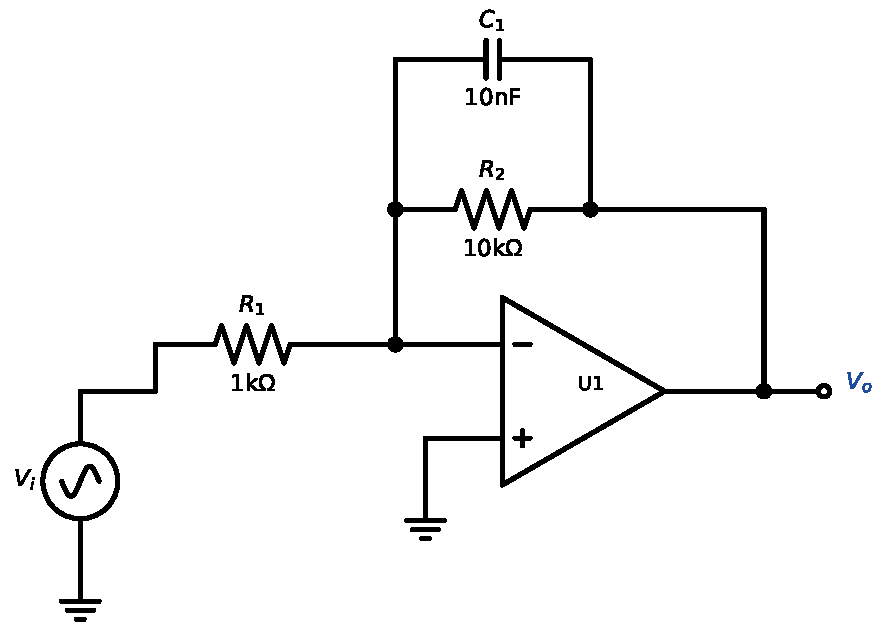
\includegraphics[width=\linewidth,height=5.6cm,keepaspectratio]{p01_circuit}\end{center}
\end{probbox}

\begin{probbox}{Problem 2A.2 \hfill Easy}
For the circuit below (ideal op-amps): (a) find $H(s)=\dfrac{V_o(s)}{V_i(s)}$ and sketch its magnitude Bode plot; (b) find the steady-state output $V_o(t)$ for $V_i(t) = 0.2\sin\left(2\pi\cdot 50\,t\right)$.
\begin{center}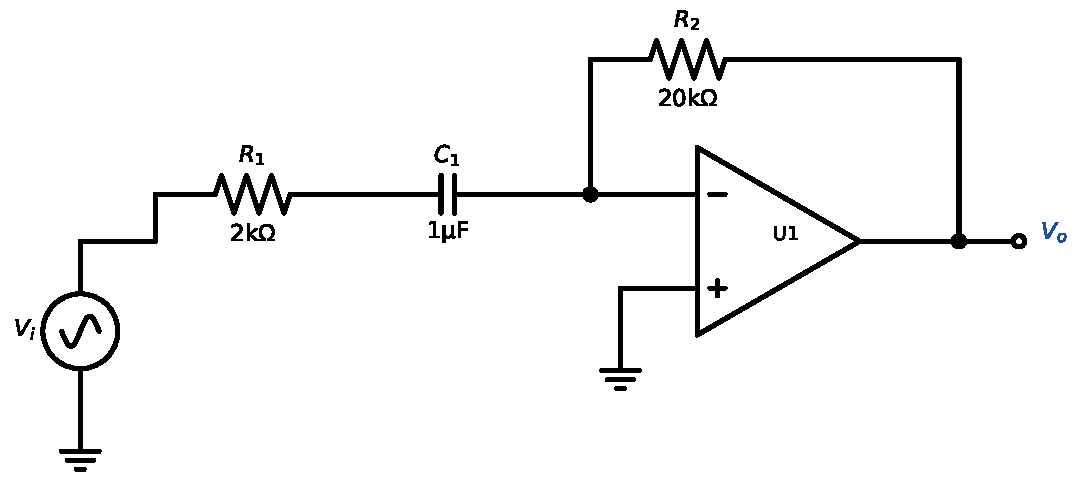
\includegraphics[width=\linewidth,height=5.6cm,keepaspectratio]{p02_circuit}\end{center}
\end{probbox}

\begin{probbox}{Problem 2A.3 \hfill Easy}
For the circuit below (ideal op-amps): (a) find $H(s)=\dfrac{V_o(s)}{V_i(s)}$ and sketch its magnitude Bode plot; (b) find the steady-state output $V_o(t)$ for $V_i(t) = 0.1\sin\left(2\pi\cdot 5000\,t\right)$.
\begin{center}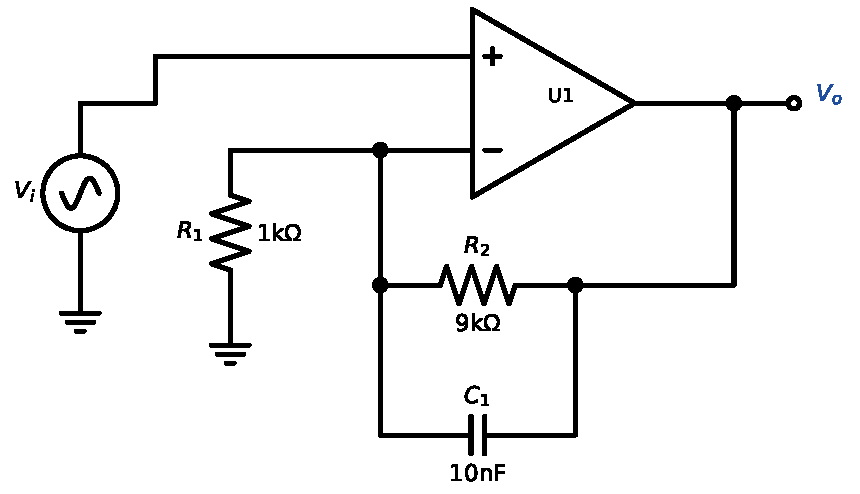
\includegraphics[width=\linewidth,height=5.6cm,keepaspectratio]{p03_circuit}\end{center}
\end{probbox}

\begin{probbox}{Problem 2A.4 \hfill Easy}
For the circuit below (ideal op-amps): (a) find $H(s)=\dfrac{V_o(s)}{V_i(s)}$ and sketch its magnitude Bode plot; (b) find the steady-state output $V_o(t)$ for $V_i(t) = 0.2\sin\left(2\pi\cdot 100\,t\right)$.
\begin{center}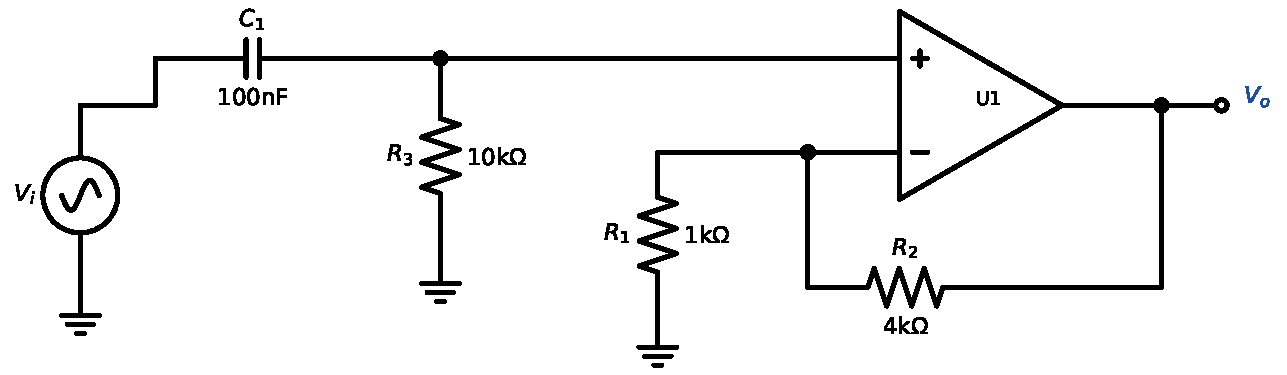
\includegraphics[width=\linewidth,height=5.6cm,keepaspectratio]{p04_circuit}\end{center}
\end{probbox}

\begin{probbox}{Problem 2A.5 \hfill Easy}
For the circuit below (ideal op-amps): (a) find $H(s)=\dfrac{V_o(s)}{V_i(s)}$ and sketch its magnitude Bode plot; (b) find the steady-state output $V_o(t)$ for $V_i(t) = 0.05\sin\left(2\pi\cdot 1000\,t\right)$.
\begin{center}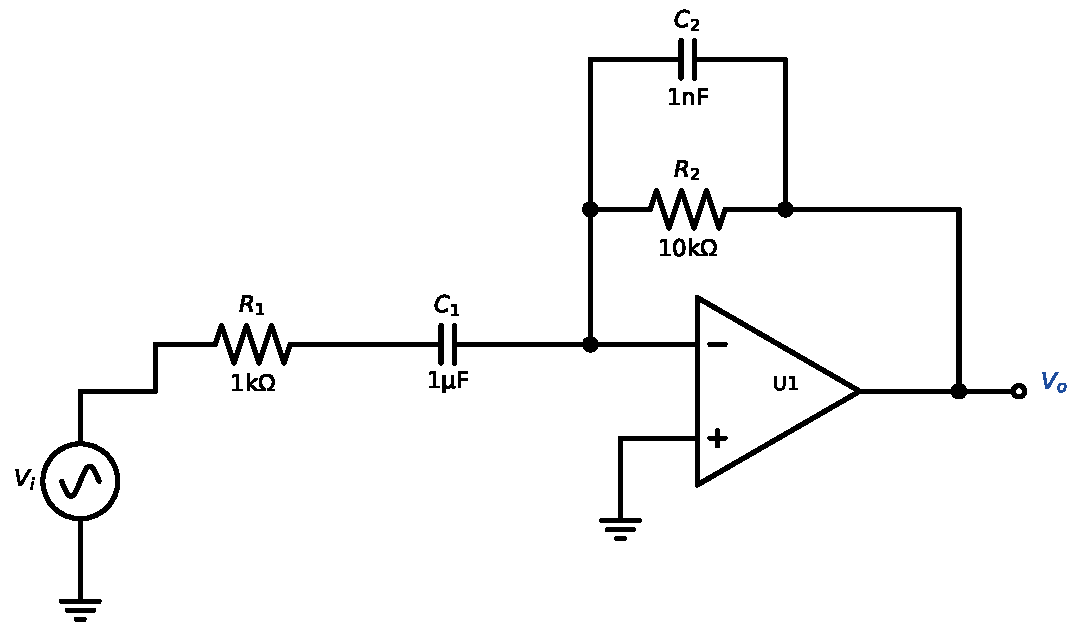
\includegraphics[width=\linewidth,height=5.6cm,keepaspectratio]{p05_circuit}\end{center}
\end{probbox}

\begin{probbox}{Problem 2A.6 \hfill Easy}
For the circuit below (ideal op-amps): (a) find $H(s)=\dfrac{V_o(s)}{V_i(s)}$ and sketch its magnitude Bode plot; (b) find the steady-state output $V_o(t)$ for $V_i(t) = 1\cos\left(2\pi\cdot 3000\,t\right)$.
\begin{center}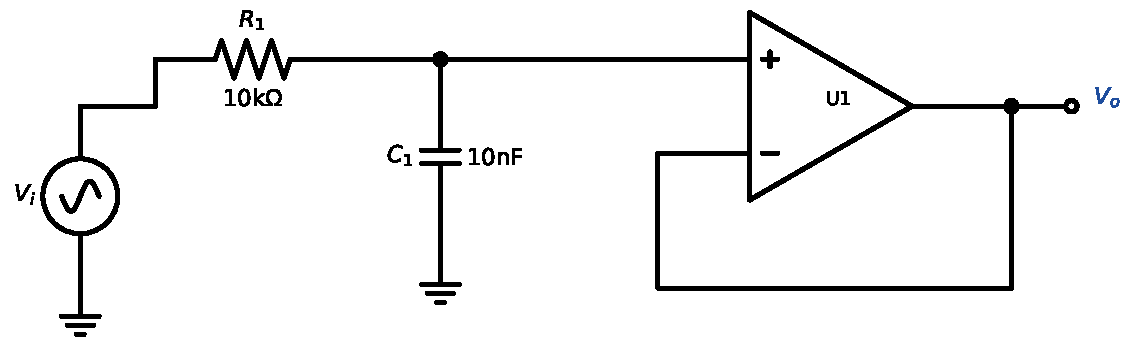
\includegraphics[width=\linewidth,height=5.6cm,keepaspectratio]{p06_circuit}\end{center}
\end{probbox}

\subsection*{Medium problems}
\begin{probbox}{Problem 2A.7 \hfill Medium}
For the circuit below (ideal op-amps): (a) find $H(s)=\dfrac{V_o(s)}{V_i(s)}$ and sketch its magnitude Bode plot; (b) find the steady-state output $V_o(t)$ for $V_i(t) = 0.02\sin\left(2\pi\cdot 500\,t\right)$.
\begin{center}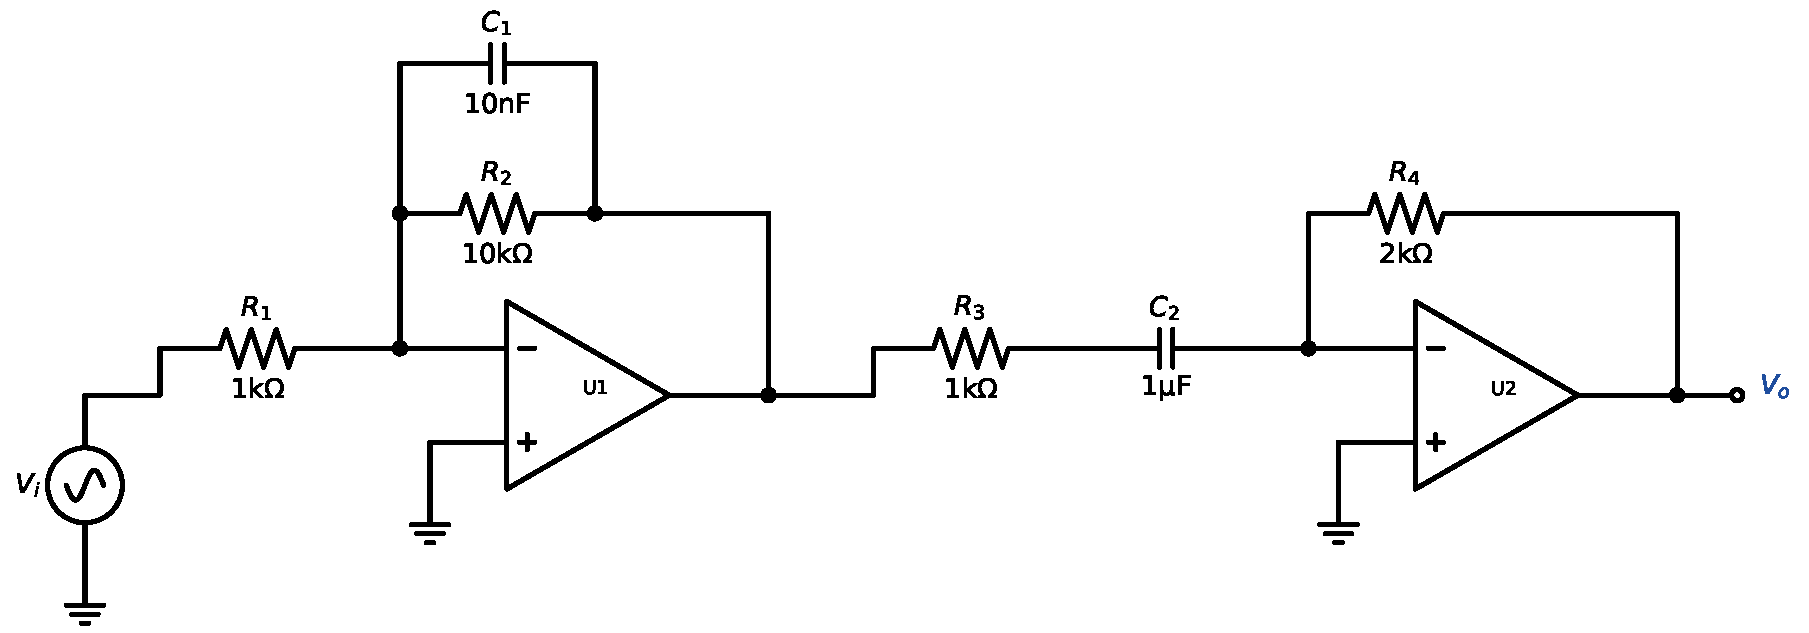
\includegraphics[width=\linewidth,height=5.6cm,keepaspectratio]{p07_circuit}\end{center}
\end{probbox}

\begin{probbox}{Problem 2A.8 \hfill Medium}
For the circuit below (ideal op-amps): (a) find $H(s)=\dfrac{V_o(s)}{V_i(s)}$ and sketch its magnitude Bode plot; (b) find the steady-state output $V_o(t)$ for $V_i(t) = 0.1\sin\left(2\pi\cdot 500\,t\right)$.
\begin{center}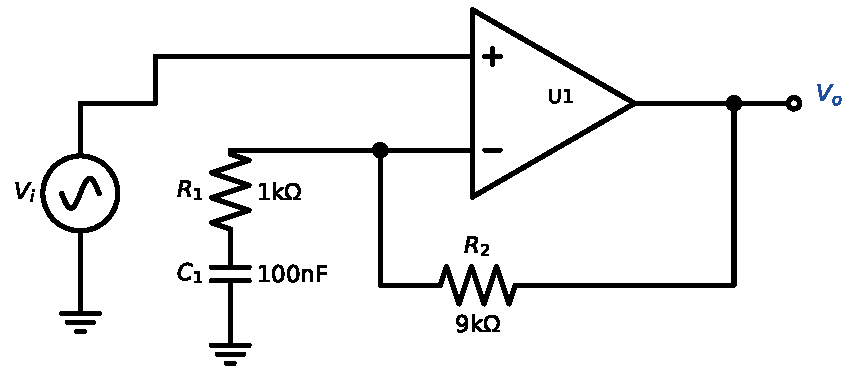
\includegraphics[width=\linewidth,height=5.6cm,keepaspectratio]{p08_circuit}\end{center}
\end{probbox}

\begin{probbox}{Problem 2A.9 \hfill Medium}
For the circuit below (ideal op-amps): (a) find $H(s)=\dfrac{V_o(s)}{V_i(s)}$ and sketch its magnitude Bode plot; (b) find the steady-state output $V_o(t)$ for $V_i(t) = 0.1\sin\left(2\pi\cdot 1000\,t\right)$.
\begin{center}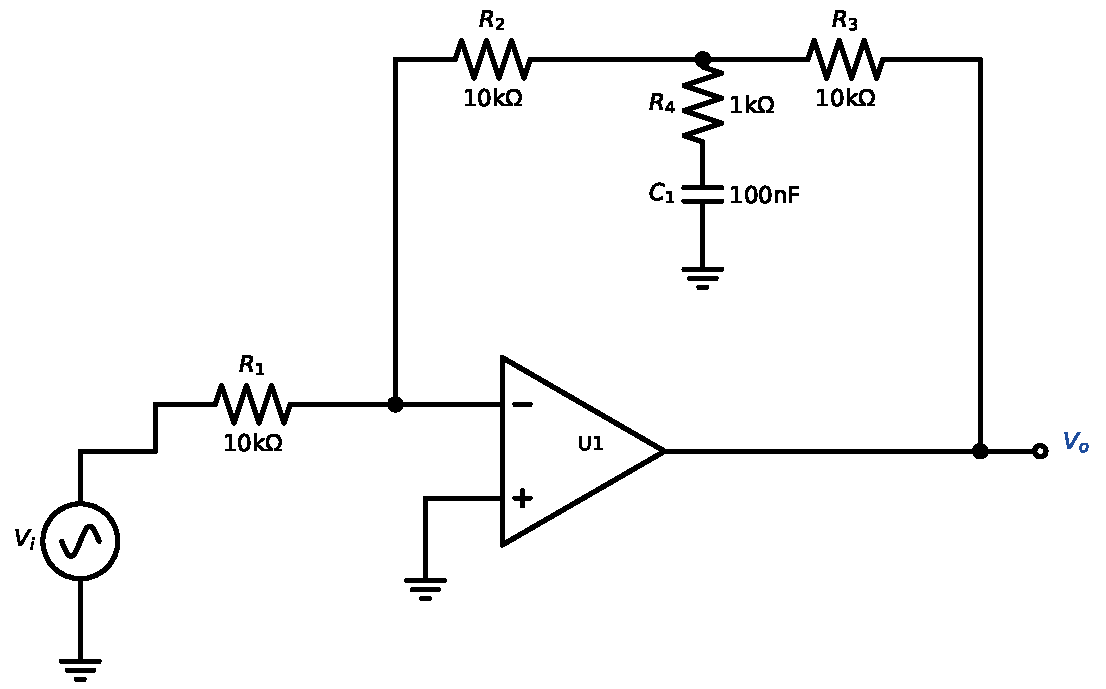
\includegraphics[width=\linewidth,height=5.6cm,keepaspectratio]{p09_circuit}\end{center}
\end{probbox}

\begin{probbox}{Problem 2A.10 \hfill Medium}
For the circuit below (ideal op-amps): (a) find $H(s)=\dfrac{V_o(s)}{V_i(s)}$ and sketch its magnitude Bode plot; (b) find the steady-state output $V_o(t)$ for $V_i(t) = 0.1\sin\left(2\pi\cdot 2000\,t\right)$.
\begin{center}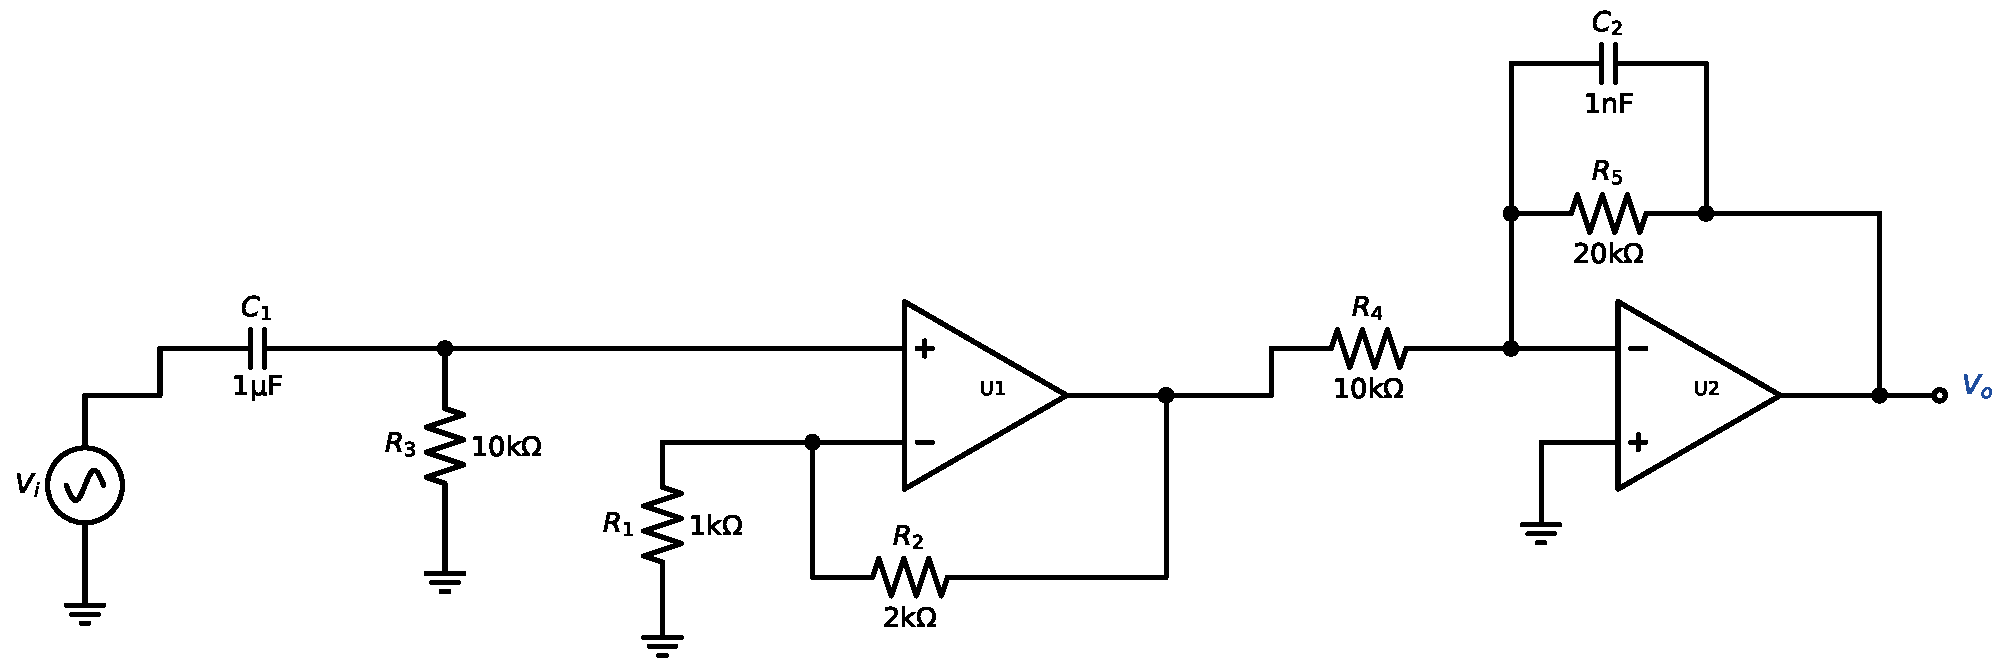
\includegraphics[width=\linewidth,height=5.6cm,keepaspectratio]{p10_circuit}\end{center}
\end{probbox}

\begin{probbox}{Problem 2A.11 \hfill Medium}
For the circuit below (ideal op-amps): (a) find $H(s)=\dfrac{V_o(s)}{V_i(s)}$ and sketch its magnitude Bode plot; (b) find the steady-state output $V_o(t)$ for $V_i(t) = 0.5\sin\left(2\pi\cdot 1000\,t\right)$.
\begin{center}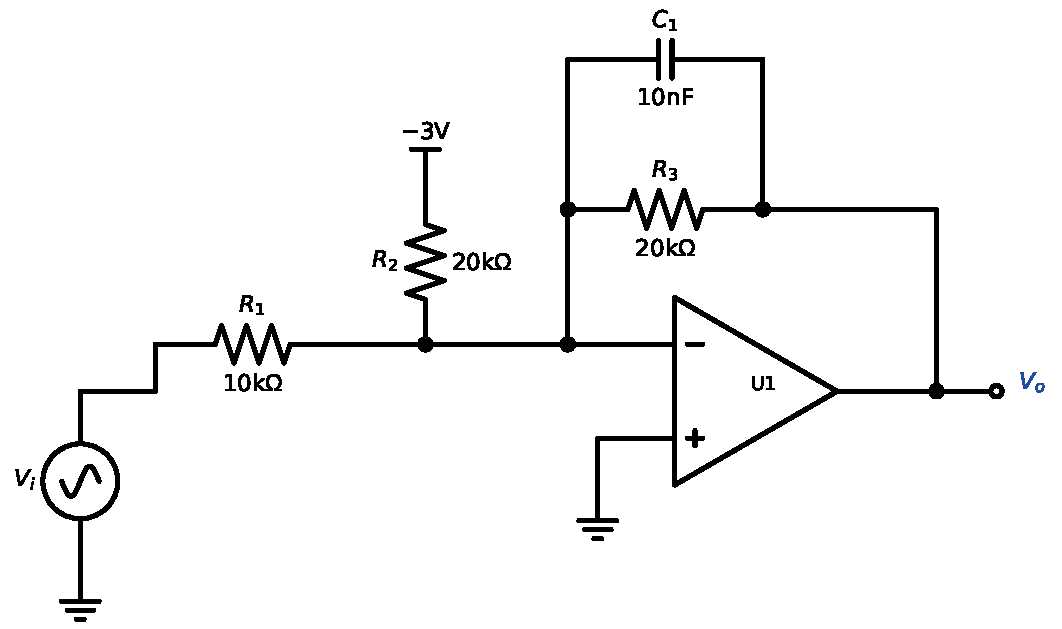
\includegraphics[width=\linewidth,height=5.6cm,keepaspectratio]{p11_circuit}\end{center}
\end{probbox}

\begin{probbox}{Problem 2A.12 \hfill Medium}
For the circuit below (ideal op-amps): (a) find $H(s)=\dfrac{V_o(s)}{V_i(s)}$ and sketch its magnitude Bode plot; (b) find the steady-state output $V_o(t)$ for $V_i(t) = 0.2\sin\left(2\pi\cdot 300\,t\right)$.
\begin{center}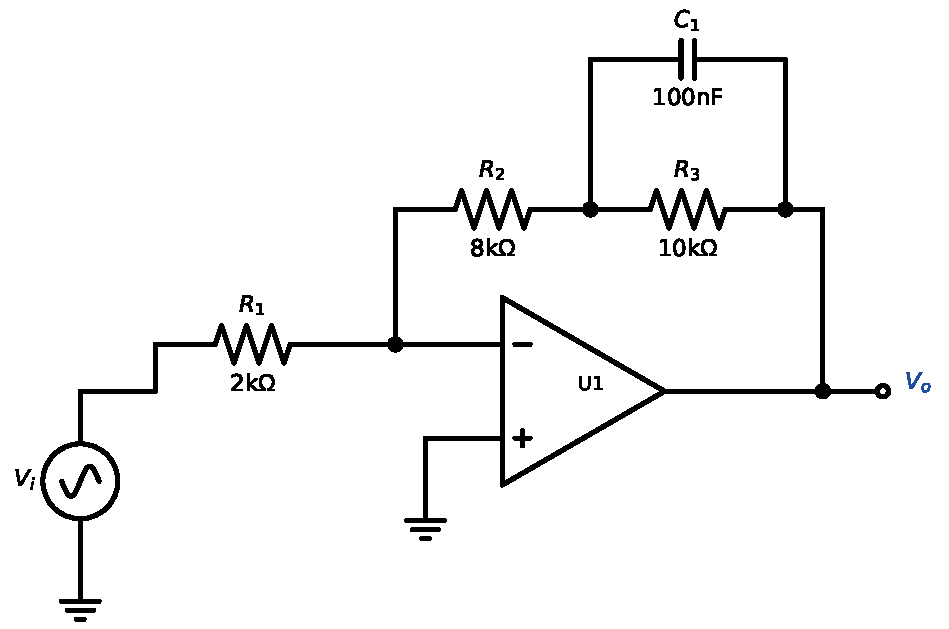
\includegraphics[width=\linewidth,height=5.6cm,keepaspectratio]{p12_circuit}\end{center}
\end{probbox}

\subsection*{Hard problems}
\begin{probbox}{Problem 2A.13 \hfill Hard}
For the circuit below (ideal op-amps): (a) find $H(s)=\dfrac{V_o(s)}{V_i(s)}$ and sketch its magnitude Bode plot; (b) find the steady-state output $V_o(t)$ for $V_i(t) = 0.01\sin\left(2\pi\cdot 2000\,t\right)$.
\begin{center}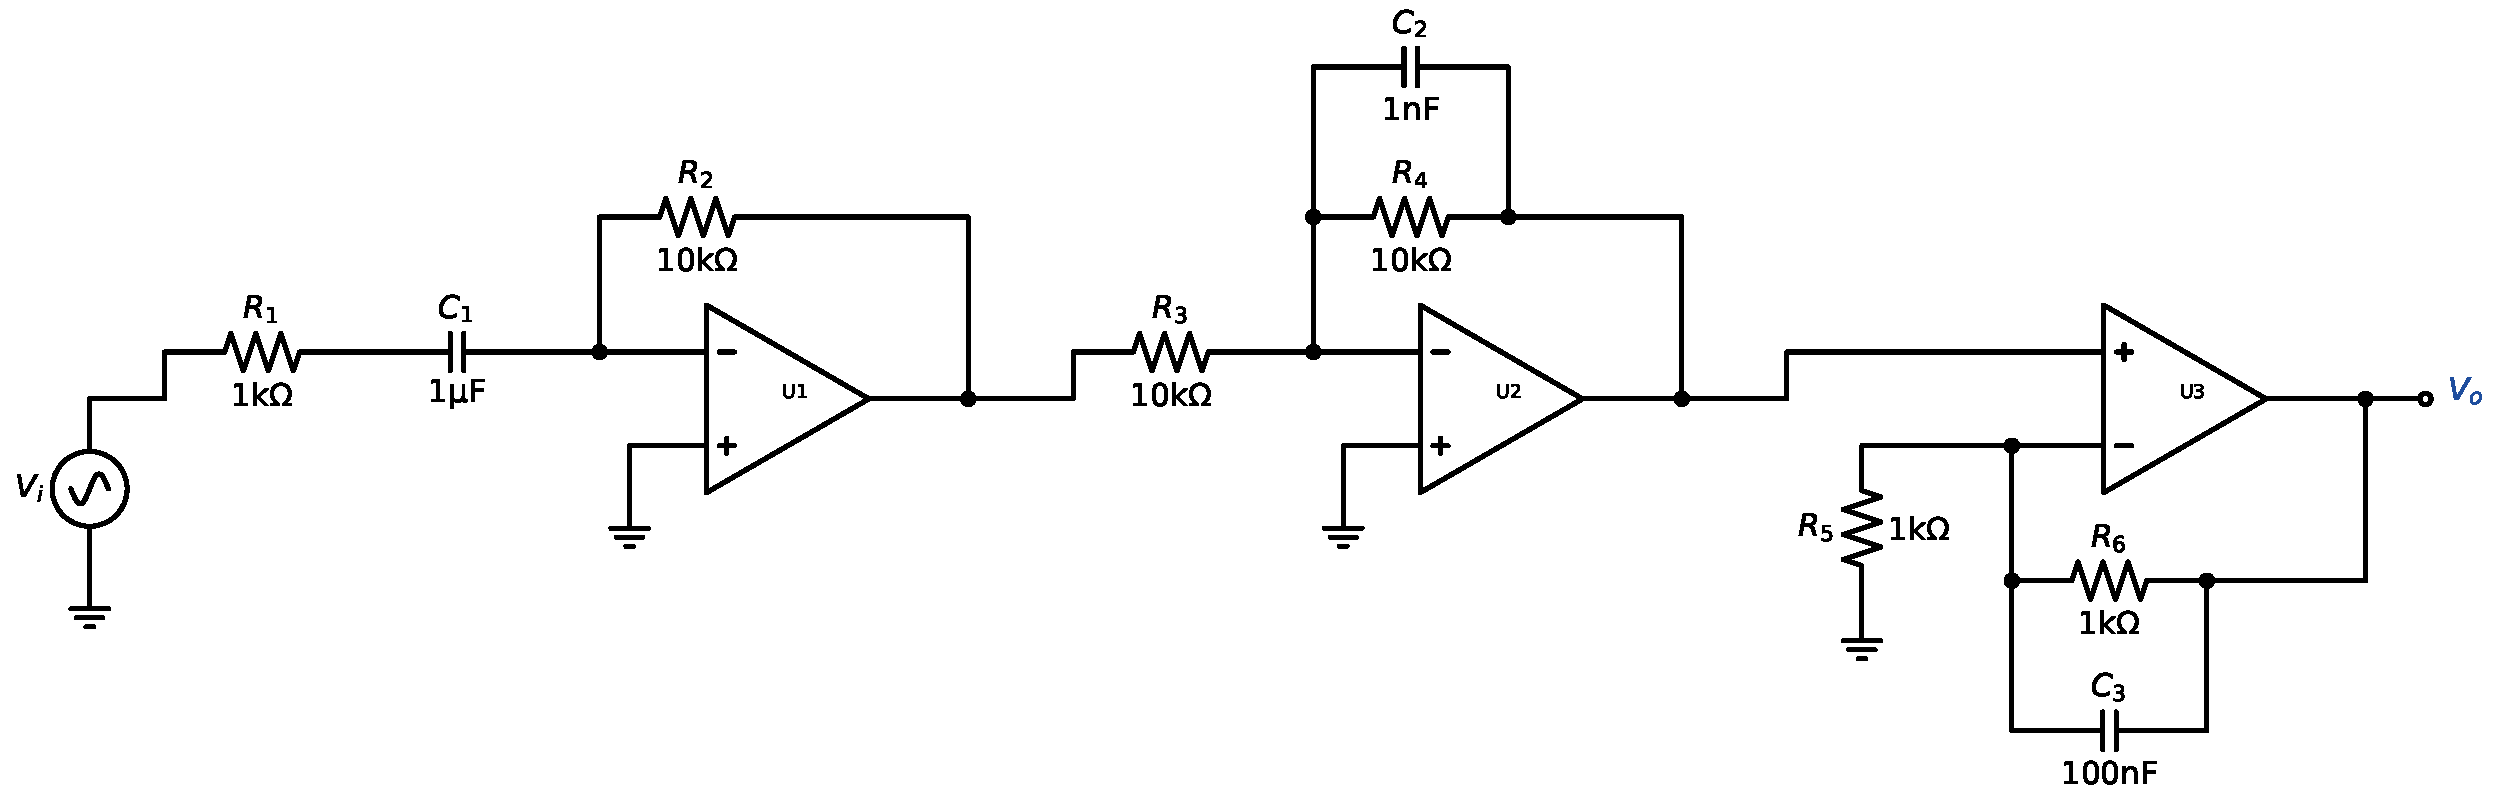
\includegraphics[width=\linewidth,height=5.6cm,keepaspectratio]{p13_circuit}\end{center}
\end{probbox}

\begin{probbox}{Problem 2A.14 \hfill Hard}
For the circuit below (ideal op-amps): (a) find $H(s)=\dfrac{V_o(s)}{V_i(s)}$ and sketch its magnitude Bode plot; (b) find the steady-state output $V_o(t)$ for $V_i(t) = 0.1\sin\left(2\pi\cdot 1000\,t+\frac{\pi}{4}\right)$.
\begin{center}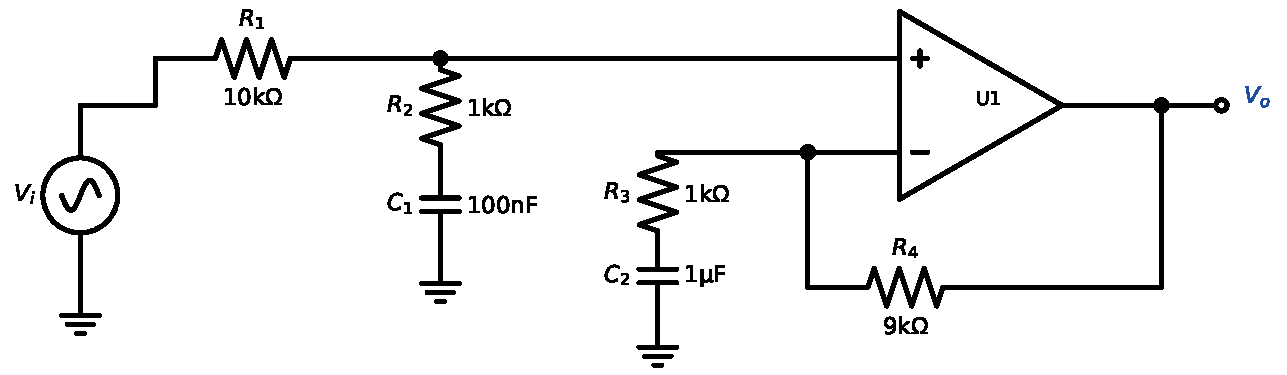
\includegraphics[width=\linewidth,height=5.6cm,keepaspectratio]{p14_circuit}\end{center}
\end{probbox}

\begin{probbox}{Problem 2A.15 \hfill Hard}
For the circuit below (ideal op-amps): (a) find $H(s)=\dfrac{V_o(s)}{V_i(s)}$ and sketch its magnitude Bode plot; (b) find the steady-state output $V_o(t)$ for $V_i(t) = 0.05\sin\left(2\pi\cdot 1000\,t\right)$. (The DC supply in the first block is $+2\,\mathrm{V}$.)
\begin{center}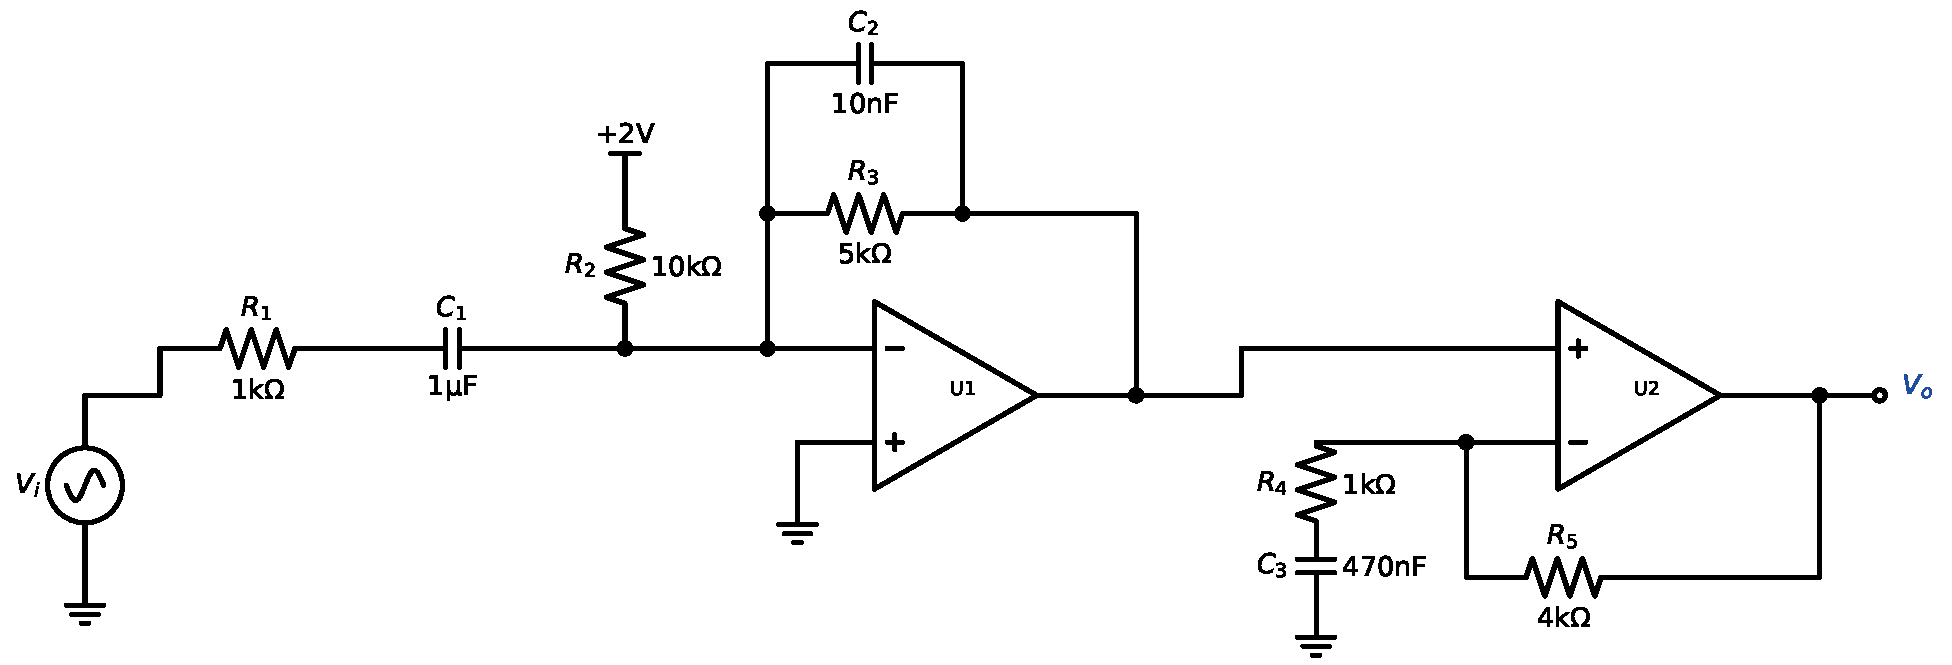
\includegraphics[width=\linewidth,height=5.6cm,keepaspectratio]{p15_circuit}\end{center}
\end{probbox}

\begin{probbox}{Problem 2A.16 \hfill Hard}
For the circuit below (ideal op-amps): (a) find $H(s)=\dfrac{V_o(s)}{V_i(s)}$ and sketch its magnitude Bode plot; (b) find the steady-state output $V_o(t)$ for $V_i(t) = 0.01\sin\left(2\pi\cdot 2000\,t\right)$.
\begin{center}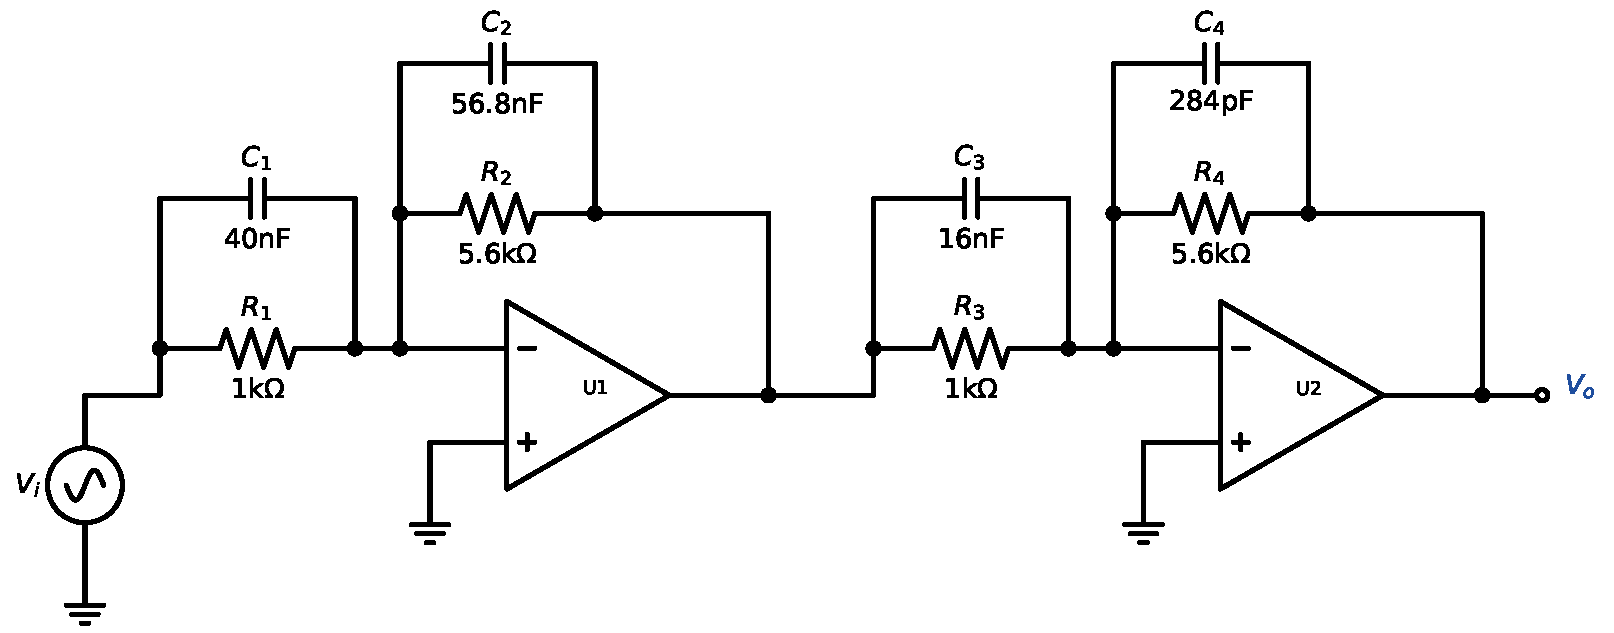
\includegraphics[width=\linewidth,height=5.6cm,keepaspectratio]{p16_circuit}\end{center}
\end{probbox}

\begin{probbox}{Problem 2A.17 \hfill Hard}
For the circuit below (ideal op-amps): (a) find $H(s)=\dfrac{V_o(s)}{V_i(s)}$ and sketch its magnitude Bode plot; (b) find the steady-state output $V_o(t)$ for $V_i(t) = 0.5\cos\left(2\pi\cdot 10000\,t-\frac{\pi}{3}\right)$.
\begin{center}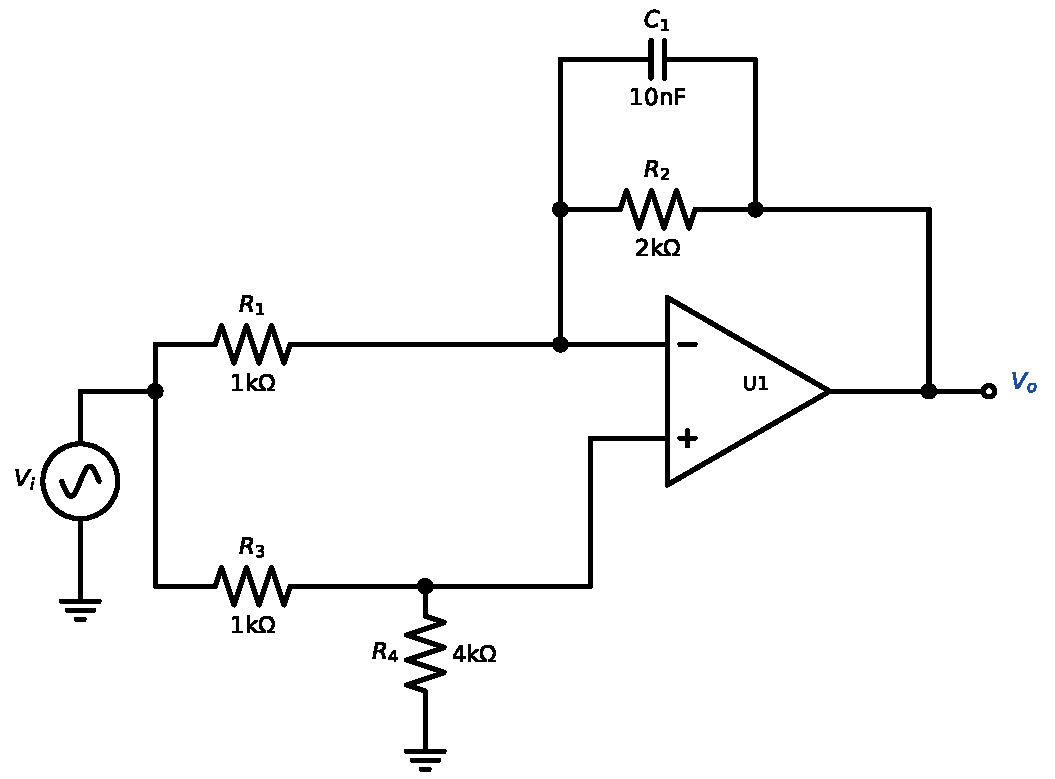
\includegraphics[width=\linewidth,height=5.6cm,keepaspectratio]{p17_circuit}\end{center}
\end{probbox}

\begin{probbox}{Problem 2A.18 \hfill Hard}
For the circuit below (ideal op-amps): (a) find $H(s)=\dfrac{V_o(s)}{V_i(s)}$ and sketch its magnitude Bode plot; (b) find the steady-state output $V_o(t)$ for $V_i(t) = 0.1\sin\left(2\pi\cdot 3000\,t+\frac{\pi}{6}\right)$.
\begin{center}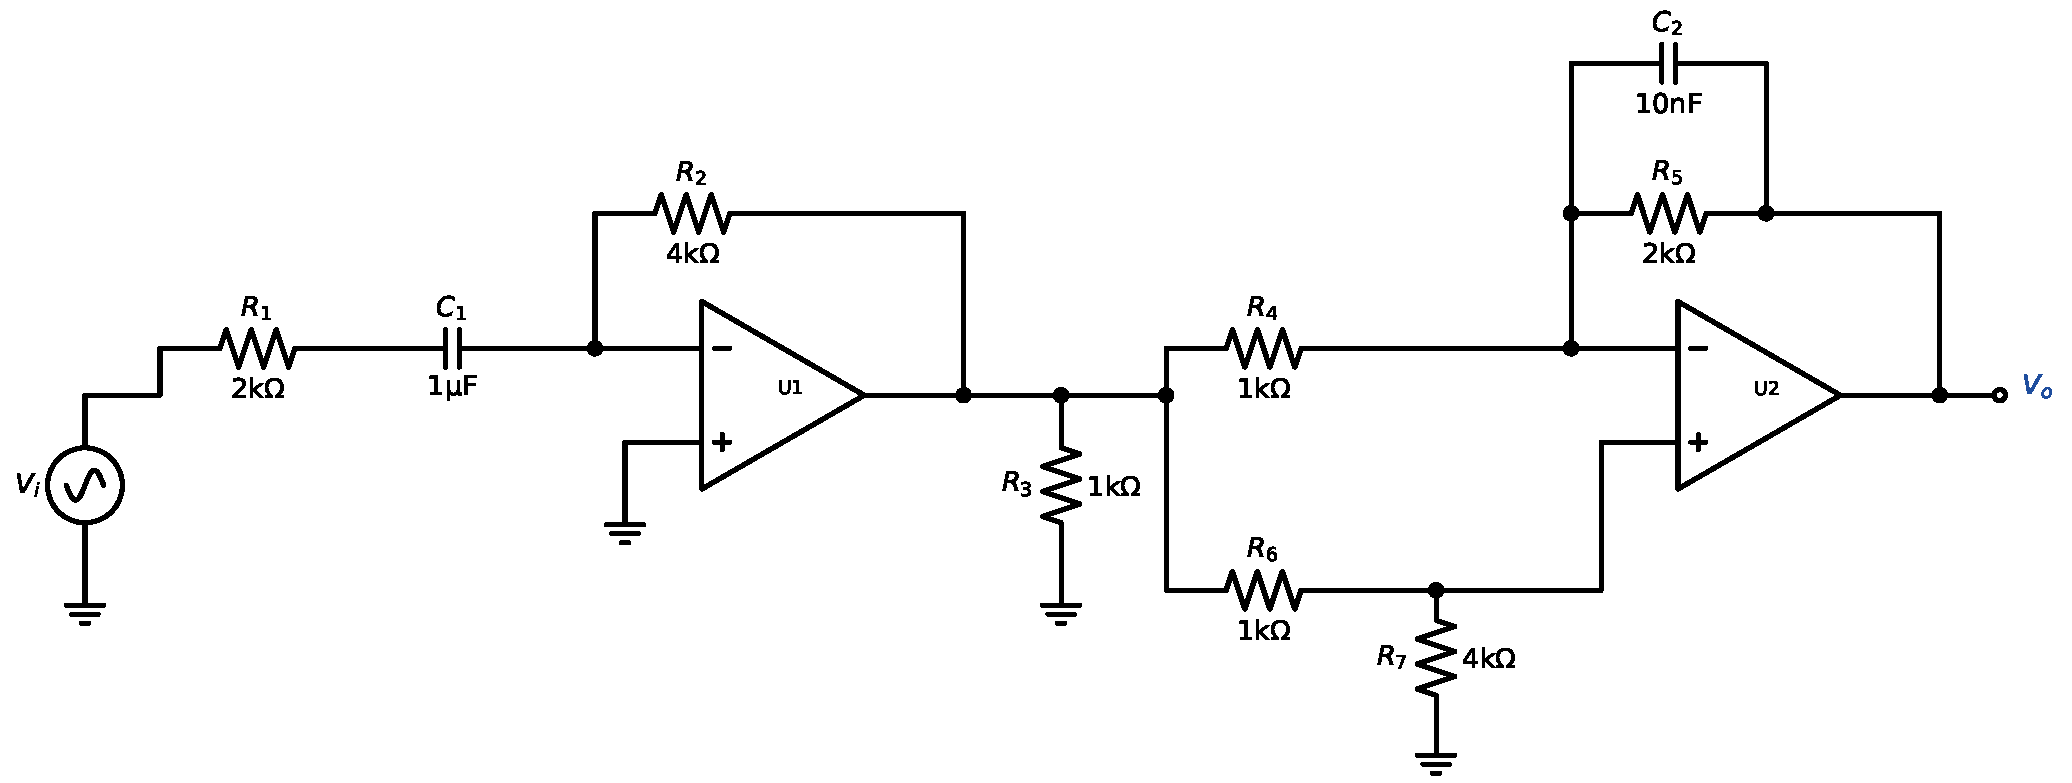
\includegraphics[width=\linewidth,height=5.6cm,keepaspectratio]{p18_circuit}\end{center}
\end{probbox}

\newpage
\section*{Solutions}
Every solution follows the steps of the Lecture-2 pipeline card.
\newpage
\subsection*{Solution 2A.1 \hfill Easy}
\begin{center}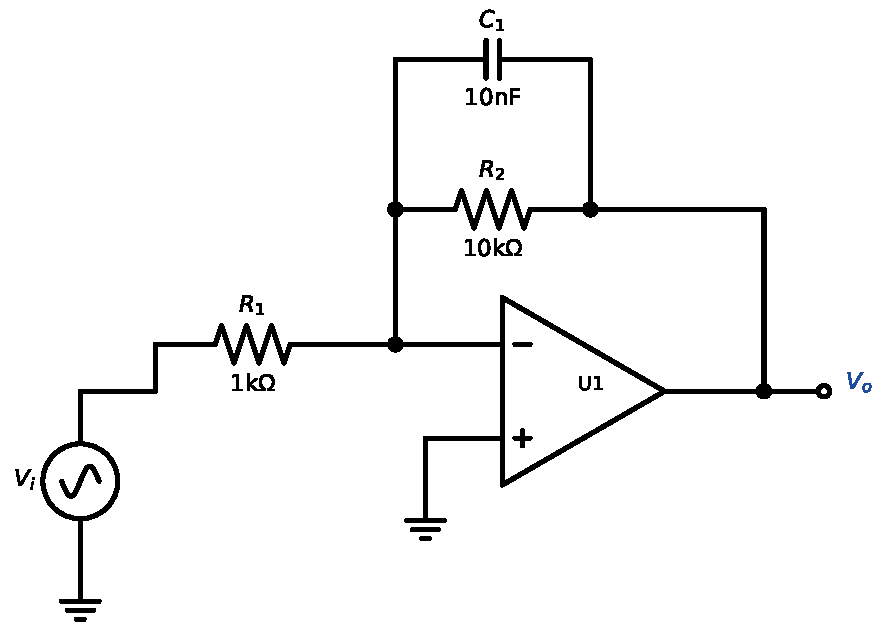
\includegraphics[width=\linewidth,height=5cm,keepaspectratio]{p01_circuit}\end{center}
\solstep{1}{Identify the sources}Independent sources: the AC input $V_i(t)$. No DC source: $V_{o,dc}=0$ and Step 2 is skipped.
\solstep{2}{DC circuit}No DC sources: $V_{o,dc}=0$.
\solstep{3}{Op-amp rules}The op-amp has negative feedback (its output is connected back to its $-$ input), so with an ideal op-amp (tool T1): (a) no current flows into the $+$ or $-$ input; (b) $V_-=V_+$ (virtual short). The circuit is a standard block, so use its block formula (tool T2).
\solstep{4}{Transfer function, block by block}\textbf{Block 1 (U1).} Inverting block: the $+$ input is grounded, so $V_- = V_+ = 0$ (virtual ground). The current $\frac{V_{i} - 0}{R_{1}}$ through $R_{1}$ cannot enter the op-amp, so all of it flows through $Z_{f1}$: $V_{o} = 0 - Z_{f1}\cdot\frac{V_{i}}{R_{1}}$.\begin{align*}
Z_{f1} &= R_{2} \parallel \frac{1}{sC_{1}} = \dfrac{10^{8}}{s + 10000}
\end{align*}
\[
\frac{V_{o}}{V_{i}} = -\frac{Z_{f1}}{R_{1}} = \dfrac{-10^{5}}{s + 10000}
\]

So:\[
H(s) = \dfrac{-10^{5}}{s + 10000}
\]

\solstep{5}{Standard (Bode-ready) form}Find the roots. Every root $s=-p$ of the denominator is a \emph{pole}, every root $s=-z$ of the numerator is a \emph{zero}; $|p|$ and $|z|$ are the corner frequencies (rad/s).
\begin{itemize}[leftmargin=*,itemsep=2pt]
\item Denominator: $s + 10000$; $s + 10000 = 0 \Rightarrow s = -10000$.
\end{itemize}

Factored form (leading coefficient in front):
\[
H(s) = -10^{5}\,\dfrac{1}{(s+10000)}
\]

Bode-ready form: rewrite every $(s+p) = p\left(1+\frac{s}{p}\right)$ and $(s+z) = z\left(1+\frac{s}{z}\right)$, and collect all constants into $K$. Then every factor except $K$ is $\approx 1$ inside the pass-band:
\[
H(s) = -10\,\dfrac{1}{1+\dfrac{s}{2\pi\cdot 1.59\mathrm{k}}},\qquad K = -10
\]

\begin{center}\renewcommand{\arraystretch}{1.35}
\begin{tabular}{cccc}
\toprule
type & $\omega_c$ (rad/s) & $f_c=\omega_c/2\pi$ & slope change \\
\midrule
pole & $10000$ & 1.59 kHz & $-20$ dB/dec \\
\bottomrule
\end{tabular}\end{center}

\solstep{6}{Magnitude Bode plot}Below every corner, all factors are $\approx$ constant: $|H| \approx 10$ $= 20$\,dB (flat, 0 dB/dec). Then, moving right, each pole bends the line down by 20\,dB/dec and each zero bends it up by 20\,dB/dec (tool T6):
\begin{center}\renewcommand{\arraystretch}{1.35}
\begin{tabular}{lcl}
\toprule
frequency range & slope & asymptote level \\
\midrule
$f<$ 1.59 kHz & $0$ dB/dec (flat) & 20 dB at end \\
$f>$ 1.59 kHz & $-20$ dB/dec & 20 dB at start \\
\bottomrule
\end{tabular}\end{center}

The flat (pass-band) level is $20\log_{10}|K| = 20\log_{10}10 = 20$\,dB.
\begin{center}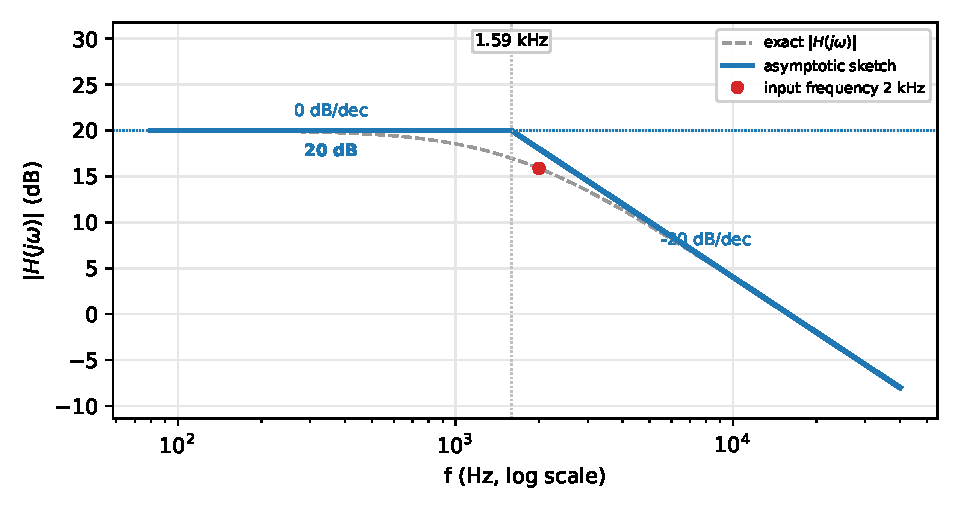
\includegraphics[width=0.78\linewidth,height=6.5cm,keepaspectratio]{p01_bode}\end{center}

{\small Blue: the straight-line sketch you are expected to draw. Dashed grey: the exact curve (about 3\,dB below the corner of an isolated pole). Red dot: the input frequency of Step 7.}
\solstep{7}{Steady-state output}The input is $V_i(t) = 0.1\sin\left(2\pi\cdot 2000\,t\right)$, so $\omega_{in} = 2\pi\cdot 2000 = 12600$\,rad/s. Put $s=j\omega_{in}$ in each factor (tool T5): magnitudes multiply, angles add.
{\small Rules: $\left|\frac{s}{s+p}\right| = \frac{\omega}{\sqrt{\omega^2+p^2}}$, $\angle = \frac{\pi}{2}-\tan^{-1}\frac{\omega}{p}$;\quad $\left|\frac{1}{1+s/p}\right| = \frac{1}{\sqrt{1+(\omega/p)^2}}$, $\angle = -\tan^{-1}\frac{\omega}{p}$;\quad $\left|1+\frac{s}{z}\right| = \sqrt{1+(\omega/z)^2}$, $\angle = \tan^{-1}\frac{\omega}{z}$;\quad a negative $K$ adds $-\pi$.}
\begin{center}\renewcommand{\arraystretch}{1.35}
\begin{tabular}{ccc}
\toprule
factor & magnitude & angle (rad) \\
\midrule
$-10$ & $10$ & $-3.14$ \\
$\rule[-1.7em]{0pt}{4em}\dfrac{1}{1+\dfrac{s}{2\pi\cdot 1.59\mathrm{k}}}$ & $0.6227$ & $-0.899$ \\
\textbf{total} & $\mathbf{6.227}$ (product) & $\mathbf{-4.04}$ (sum) \\
\bottomrule
\end{tabular}\end{center}

\begin{align*}
|H(j\omega_{in})| &= 6.23, \qquad \angle H(j\omega_{in}) = -4.04\ \mathrm{rad} \\
v_{o,ac}(t) &= 6.23\times 0.1\,\sin\left(2\pi\cdot 2000\,t - 4.04\right) = 0.623\,\sin\left(2\pi\cdot 2000\,t - 4.04\right)
\end{align*}

\[
\boxed{V_o(t) = 0.623\,\sin\left(2\pi\cdot 2000\,t - 4.04\right)\ \mathrm{V}}
\]

\begin{ansbox}
$H(s) = -10\,\dfrac{1}{1+\dfrac{s}{2\pi\cdot 1.59\mathrm{k}}}$\quad (corners: 1.59 kHz)\\[4pt]
$V_o(t) = 0.623\,\sin\left(2\pi\cdot 2000\,t - 4.04\right)\ \mathrm{V}$
\end{ansbox}

\newpage
\subsection*{Solution 2A.2 \hfill Easy}
\begin{center}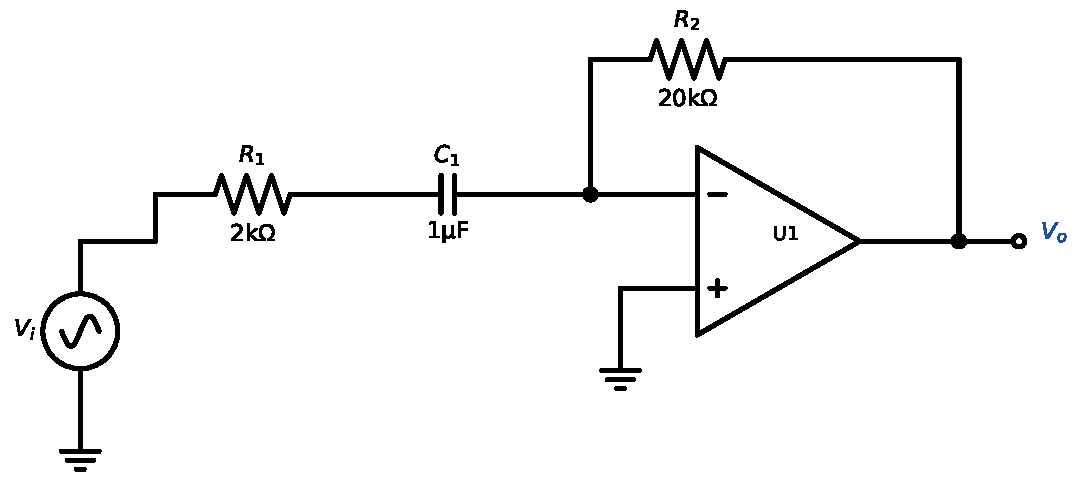
\includegraphics[width=\linewidth,height=5cm,keepaspectratio]{p02_circuit}\end{center}
\solstep{1}{Identify the sources}Independent sources: the AC input $V_i(t)$. No DC source: $V_{o,dc}=0$ and Step 2 is skipped.
\solstep{2}{DC circuit}No DC sources: $V_{o,dc}=0$.
\solstep{3}{Op-amp rules}The op-amp has negative feedback (its output is connected back to its $-$ input), so with an ideal op-amp (tool T1): (a) no current flows into the $+$ or $-$ input; (b) $V_-=V_+$ (virtual short). The circuit is a standard block, so use its block formula (tool T2).
\solstep{4}{Transfer function, block by block}\textbf{Block 1 (U1).} Inverting block: the $+$ input is grounded, so $V_- = V_+ = 0$ (virtual ground). The current $\frac{V_{i} - 0}{Z_{in1}}$ through $Z_{in1}$ cannot enter the op-amp, so all of it flows through $R_{2}$: $V_{o} = 0 - R_{2}\cdot\frac{V_{i}}{Z_{in1}}$.\begin{align*}
Z_{in1} &= R_{1} + \frac{1}{sC_{1}} = \dfrac{2000\,s + 10^{6}}{s}
\end{align*}
\[
\frac{V_{o}}{V_{i}} = -\frac{R_{2}}{Z_{in1}} = \dfrac{-10\,s}{s + 500}
\]

So:\[
H(s) = \dfrac{-10\,s}{s + 500}
\]

\solstep{5}{Standard (Bode-ready) form}Find the roots. Every root $s=-p$ of the denominator is a \emph{pole}, every root $s=-z$ of the numerator is a \emph{zero}; $|p|$ and $|z|$ are the corner frequencies (rad/s).
\begin{itemize}[leftmargin=*,itemsep=2pt]
\item Numerator: it has the factor $s$ $\Rightarrow$ 1 zero at $s=0$.
\item Denominator: $s + 500$; $s + 500 = 0 \Rightarrow s = -500$.
\end{itemize}

Factored form (leading coefficient in front):
\[
H(s) = -10\,\dfrac{s}{(s+500)}
\]

Bode-ready form: rewrite every $(s+p) = p\left(1+\frac{s}{p}\right)$ and $(s+z) = z\left(1+\frac{s}{z}\right)$, and collect all constants into $K$. Each $s$ in the numerator is paired with one of the \emph{lowest} poles as $\frac{s}{s+p}$ (that factor is $\approx 1$ above $p$). Then every factor except $K$ is $\approx 1$ inside the pass-band:
\[
H(s) = -10\,\dfrac{s}{s+2\pi\cdot 79.6},\qquad K = -10
\]

\begin{center}\renewcommand{\arraystretch}{1.35}
\begin{tabular}{cccc}
\toprule
type & $\omega_c$ (rad/s) & $f_c=\omega_c/2\pi$ & slope change \\
\midrule
pole & $500$ & 79.6 Hz & $-20$ dB/dec \\
\bottomrule
\end{tabular}\end{center}

\solstep{6}{Magnitude Bode plot}Below every corner $|H(s)|\approx 0.02\,s$, so the plot starts with a slope of $+20$\,dB/dec. Then, moving right, each pole bends the line down by 20\,dB/dec and each zero bends it up by 20\,dB/dec (tool T6):
\begin{center}\renewcommand{\arraystretch}{1.35}
\begin{tabular}{lcl}
\toprule
frequency range & slope & asymptote level \\
\midrule
$f<$ 79.6 Hz & $+20$ dB/dec & 20 dB at end \\
$f>$ 79.6 Hz & $0$ dB/dec (flat) & 20 dB at start \\
\bottomrule
\end{tabular}\end{center}

The flat (pass-band) level is $20\log_{10}|K| = 20\log_{10}10 = 20$\,dB.
\begin{center}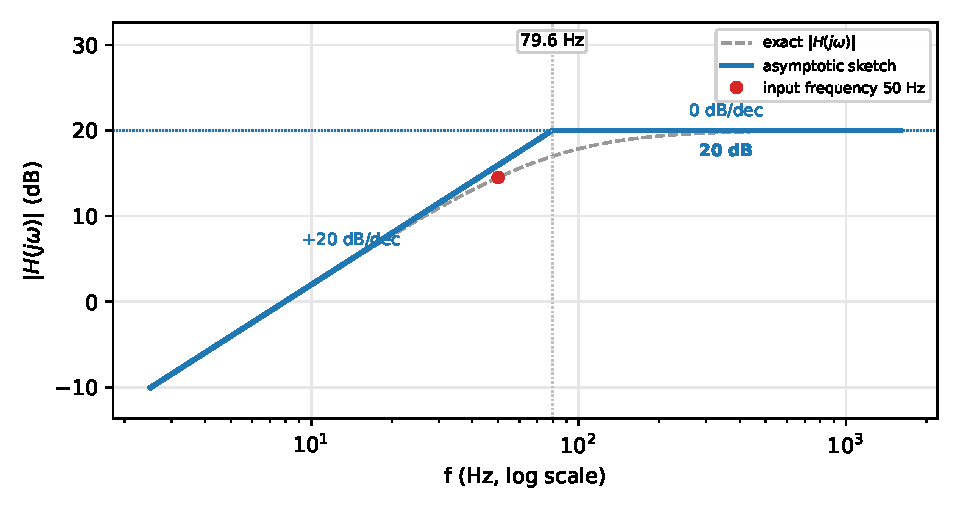
\includegraphics[width=0.78\linewidth,height=6.5cm,keepaspectratio]{p02_bode}\end{center}

{\small Blue: the straight-line sketch you are expected to draw. Dashed grey: the exact curve (about 3\,dB below the corner of an isolated pole). Red dot: the input frequency of Step 7.}
\solstep{7}{Steady-state output}The input is $V_i(t) = 0.2\sin\left(2\pi\cdot 50\,t\right)$, so $\omega_{in} = 2\pi\cdot 50 = 314$\,rad/s. Put $s=j\omega_{in}$ in each factor (tool T5): magnitudes multiply, angles add.
{\small Rules: $\left|\frac{s}{s+p}\right| = \frac{\omega}{\sqrt{\omega^2+p^2}}$, $\angle = \frac{\pi}{2}-\tan^{-1}\frac{\omega}{p}$;\quad $\left|\frac{1}{1+s/p}\right| = \frac{1}{\sqrt{1+(\omega/p)^2}}$, $\angle = -\tan^{-1}\frac{\omega}{p}$;\quad $\left|1+\frac{s}{z}\right| = \sqrt{1+(\omega/z)^2}$, $\angle = \tan^{-1}\frac{\omega}{z}$;\quad a negative $K$ adds $-\pi$.}
\begin{center}\renewcommand{\arraystretch}{1.35}
\begin{tabular}{ccc}
\toprule
factor & magnitude & angle (rad) \\
\midrule
$-10$ & $10$ & $-3.14$ \\
$\rule[-1.1em]{0pt}{2.8em}\dfrac{s}{s+2\pi\cdot 79.6}$ & $0.532$ & $1.01$ \\
\textbf{total} & $\mathbf{5.32}$ (product) & $\mathbf{-2.13}$ (sum) \\
\bottomrule
\end{tabular}\end{center}

\begin{align*}
|H(j\omega_{in})| &= 5.32, \qquad \angle H(j\omega_{in}) = -2.13\ \mathrm{rad} \\
v_{o,ac}(t) &= 5.32\times 0.2\,\sin\left(2\pi\cdot 50\,t - 2.13\right) = 1.06\,\sin\left(2\pi\cdot 50\,t - 2.13\right)
\end{align*}

\[
\boxed{V_o(t) = 1.06\,\sin\left(2\pi\cdot 50\,t - 2.13\right)\ \mathrm{V}}
\]

\begin{ansbox}
$H(s) = -10\,\dfrac{s}{s+2\pi\cdot 79.6}$\quad (corners: 79.6 Hz)\\[4pt]
$V_o(t) = 1.06\,\sin\left(2\pi\cdot 50\,t - 2.13\right)\ \mathrm{V}$
\end{ansbox}

\newpage
\subsection*{Solution 2A.3 \hfill Easy}
\begin{center}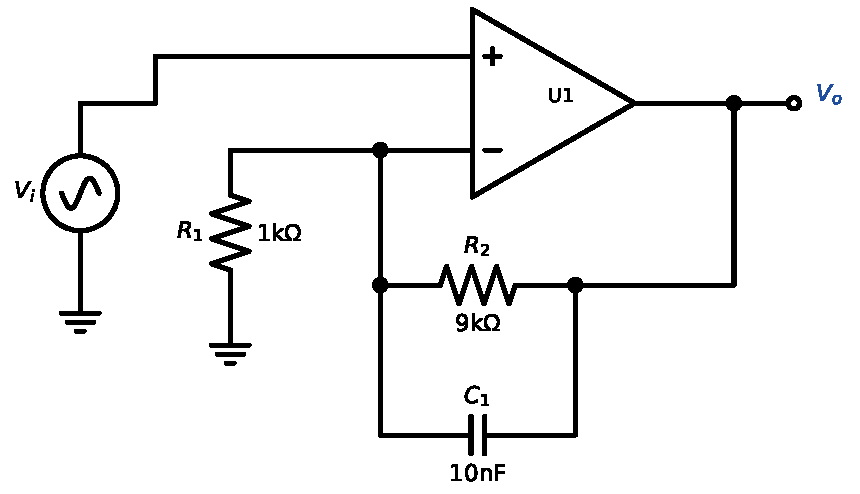
\includegraphics[width=\linewidth,height=5cm,keepaspectratio]{p03_circuit}\end{center}
\solstep{1}{Identify the sources}Independent sources: the AC input $V_i(t)$. No DC source: $V_{o,dc}=0$ and Step 2 is skipped.
\solstep{2}{DC circuit}No DC sources: $V_{o,dc}=0$.
\solstep{3}{Op-amp rules}The op-amp has negative feedback (its output is connected back to its $-$ input), so with an ideal op-amp (tool T1): (a) no current flows into the $+$ or $-$ input; (b) $V_-=V_+$ (virtual short). The circuit is a standard block, so use its block formula (tool T2).
\solstep{4}{Transfer function, block by block}\textbf{Block 1 (U1).} Non-inverting block: The $+$ input is the block input: $V_+ = V_{i}$. The op-amp forces $V_-=V_+$, and $R_{1}$, $Z_{f1}$ divide the output: $V_- = \frac{R_{1}}{R_{1} + Z_{f1}}V_{o}$, hence $V_{o} = \left(1+\frac{Z_{f1}}{R_{1}}\right)V_+$.\begin{align*}
Z_{f1} &= R_{2} \parallel \frac{1}{sC_{1}} = \dfrac{10^{8}}{s + 11100}
\end{align*}
\[
\frac{V_{o}}{V_{i}} = \left(1+\frac{Z_{f1}}{R_{1}}\right) = \dfrac{s + 1.11\times 10^{5}}{s + 11100}
\]

So:\[
H(s) = \dfrac{s + 1.11\times 10^{5}}{s + 11100}
\]

\solstep{5}{Standard (Bode-ready) form}Find the roots. Every root $s=-p$ of the denominator is a \emph{pole}, every root $s=-z$ of the numerator is a \emph{zero}; $|p|$ and $|z|$ are the corner frequencies (rad/s).
\begin{itemize}[leftmargin=*,itemsep=2pt]
\item Numerator: $s + 1.11\times 10^{5}$; $s + 1.11\times 10^{5} = 0 \Rightarrow s = -1.11\times 10^{5}$.
\item Denominator: $s + 11100$; $s + 11100 = 0 \Rightarrow s = -11100$.
\end{itemize}

Factored form (leading coefficient in front):
\[
H(s) = 1\,\dfrac{(s+1.11\times 10^{5})}{(s+11100)}
\]

Bode-ready form: rewrite every $(s+p) = p\left(1+\frac{s}{p}\right)$ and $(s+z) = z\left(1+\frac{s}{z}\right)$, and collect all constants into $K$. Then every factor except $K$ is $\approx 1$ inside the pass-band:
\[
H(s) = 10\,\dfrac{1}{1+\dfrac{s}{2\pi\cdot 1.77\mathrm{k}}}\,\left(1+\dfrac{s}{2\pi\cdot 17.7\mathrm{k}}\right),\qquad K = 10
\]

\begin{center}\renewcommand{\arraystretch}{1.35}
\begin{tabular}{cccc}
\toprule
type & $\omega_c$ (rad/s) & $f_c=\omega_c/2\pi$ & slope change \\
\midrule
pole & $11100$ & 1.77 kHz & $-20$ dB/dec \\
zero & $1.11\times 10^{5}$ & 17.7 kHz & $+20$ dB/dec \\
\bottomrule
\end{tabular}\end{center}

\solstep{6}{Magnitude Bode plot}Below every corner, all factors are $\approx$ constant: $|H| \approx 10$ $= 20$\,dB (flat, 0 dB/dec). Then, moving right, each pole bends the line down by 20\,dB/dec and each zero bends it up by 20\,dB/dec (tool T6):
\begin{center}\renewcommand{\arraystretch}{1.35}
\begin{tabular}{lcl}
\toprule
frequency range & slope & asymptote level \\
\midrule
$f<$ 1.77 kHz & $0$ dB/dec (flat) & 20 dB at end \\
1.77 kHz -- 17.7 kHz & $-20$ dB/dec & 20 dB at start, 0 dB at end \\
$f>$ 17.7 kHz & $0$ dB/dec (flat) & 0 dB at start \\
\bottomrule
\end{tabular}\end{center}

\begin{center}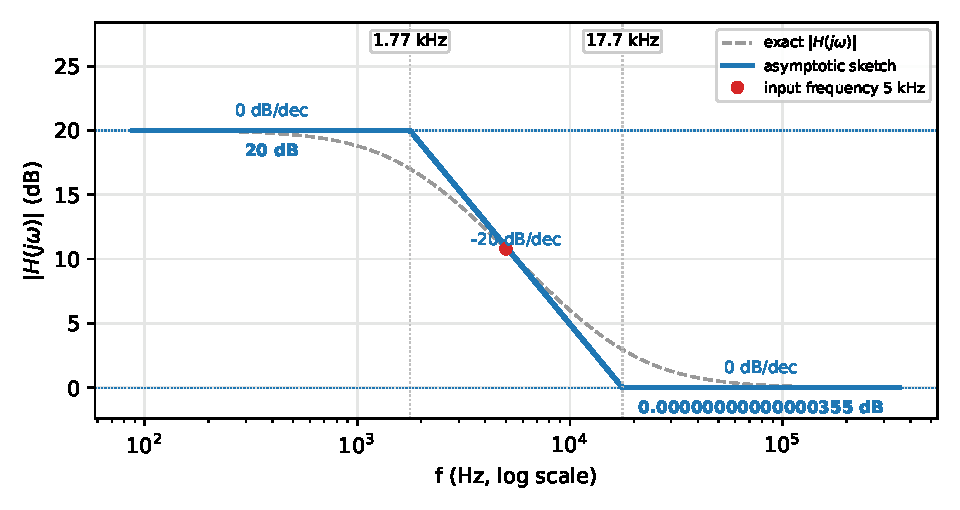
\includegraphics[width=0.78\linewidth,height=6.5cm,keepaspectratio]{p03_bode}\end{center}

{\small Blue: the straight-line sketch you are expected to draw. Dashed grey: the exact curve (about 3\,dB below the corner of an isolated pole). Red dot: the input frequency of Step 7.}
\solstep{7}{Steady-state output}The input is $V_i(t) = 0.1\sin\left(2\pi\cdot 5000\,t\right)$, so $\omega_{in} = 2\pi\cdot 5000 = 31400$\,rad/s. Put $s=j\omega_{in}$ in each factor (tool T5): magnitudes multiply, angles add.
{\small Rules: $\left|\frac{s}{s+p}\right| = \frac{\omega}{\sqrt{\omega^2+p^2}}$, $\angle = \frac{\pi}{2}-\tan^{-1}\frac{\omega}{p}$;\quad $\left|\frac{1}{1+s/p}\right| = \frac{1}{\sqrt{1+(\omega/p)^2}}$, $\angle = -\tan^{-1}\frac{\omega}{p}$;\quad $\left|1+\frac{s}{z}\right| = \sqrt{1+(\omega/z)^2}$, $\angle = \tan^{-1}\frac{\omega}{z}$;\quad a negative $K$ adds $-\pi$.}
\begin{center}\renewcommand{\arraystretch}{1.35}
\begin{tabular}{ccc}
\toprule
factor & magnitude & angle (rad) \\
\midrule
$10$ & $10$ & $0$ \\
$\rule[-1.7em]{0pt}{4em}\dfrac{1}{1+\dfrac{s}{2\pi\cdot 1.77\mathrm{k}}}$ & $0.3334$ & $-1.23$ \\
$\rule[-1.1em]{0pt}{2.8em}\left(1+\dfrac{s}{2\pi\cdot 17.7\mathrm{k}}\right)$ & $1.039$ & $0.276$ \\
\textbf{total} & $\mathbf{3.465}$ (product) & $\mathbf{-0.955}$ (sum) \\
\bottomrule
\end{tabular}\end{center}

\begin{align*}
|H(j\omega_{in})| &= 3.47, \qquad \angle H(j\omega_{in}) = -0.955\ \mathrm{rad} \\
v_{o,ac}(t) &= 3.47\times 0.1\,\sin\left(2\pi\cdot 5000\,t - 0.955\right) = 0.347\,\sin\left(2\pi\cdot 5000\,t - 0.955\right)
\end{align*}

\[
\boxed{V_o(t) = 0.347\,\sin\left(2\pi\cdot 5000\,t - 0.955\right)\ \mathrm{V}}
\]

\begin{ansbox}
$H(s) = 10\,\dfrac{1}{1+\dfrac{s}{2\pi\cdot 1.77\mathrm{k}}}\,\left(1+\dfrac{s}{2\pi\cdot 17.7\mathrm{k}}\right)$\quad (corners: 1.77 kHz, 17.7 kHz)\\[4pt]
$V_o(t) = 0.347\,\sin\left(2\pi\cdot 5000\,t - 0.955\right)\ \mathrm{V}$
\end{ansbox}

\newpage
\subsection*{Solution 2A.4 \hfill Easy}
\begin{center}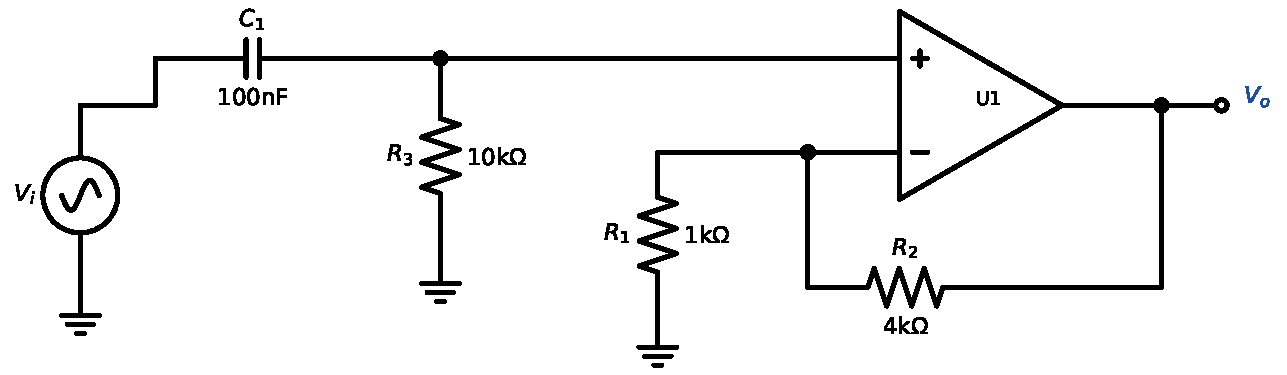
\includegraphics[width=\linewidth,height=5cm,keepaspectratio]{p04_circuit}\end{center}
\solstep{1}{Identify the sources}Independent sources: the AC input $V_i(t)$. No DC source: $V_{o,dc}=0$ and Step 2 is skipped.
\solstep{2}{DC circuit}No DC sources: $V_{o,dc}=0$.
\solstep{3}{Op-amp rules}The op-amp has negative feedback (its output is connected back to its $-$ input), so with an ideal op-amp (tool T1): (a) no current flows into the $+$ or $-$ input; (b) $V_-=V_+$ (virtual short). The circuit is a standard block, so use its block formula (tool T2).
\solstep{4}{Transfer function, block by block}\textbf{Block 1 (U1).} Non-inverting block: No current flows into the $+$ input, so $R_{3}$ and $\frac{1}{sC_{1}}$ form a plain voltage divider: $V_+ = \frac{R_{3}}{\frac{1}{sC_{1}} + R_{3}}V_{i}$. The op-amp forces $V_-=V_+$, and $R_{1}$, $R_{2}$ divide the output: $V_- = \frac{R_{1}}{R_{1} + R_{2}}V_{o}$, hence $V_{o} = \left(1+\frac{R_{2}}{R_{1}}\right)V_+$.\[
\frac{V_{o}}{V_{i}} = \frac{R_{3}}{\frac{1}{sC_{1}} + R_{3}}\left(1+\frac{R_{2}}{R_{1}}\right) = \dfrac{5\,s}{s + 1000}
\]

So:\[
H(s) = \dfrac{5\,s}{s + 1000}
\]

\solstep{5}{Standard (Bode-ready) form}Find the roots. Every root $s=-p$ of the denominator is a \emph{pole}, every root $s=-z$ of the numerator is a \emph{zero}; $|p|$ and $|z|$ are the corner frequencies (rad/s).
\begin{itemize}[leftmargin=*,itemsep=2pt]
\item Numerator: it has the factor $s$ $\Rightarrow$ 1 zero at $s=0$.
\item Denominator: $s + 1000$; $s + 1000 = 0 \Rightarrow s = -1000$.
\end{itemize}

Factored form (leading coefficient in front):
\[
H(s) = 5\,\dfrac{s}{(s+1000)}
\]

Bode-ready form: rewrite every $(s+p) = p\left(1+\frac{s}{p}\right)$ and $(s+z) = z\left(1+\frac{s}{z}\right)$, and collect all constants into $K$. Each $s$ in the numerator is paired with one of the \emph{lowest} poles as $\frac{s}{s+p}$ (that factor is $\approx 1$ above $p$). Then every factor except $K$ is $\approx 1$ inside the pass-band:
\[
H(s) = 5\,\dfrac{s}{s+2\pi\cdot 159},\qquad K = 5
\]

\begin{center}\renewcommand{\arraystretch}{1.35}
\begin{tabular}{cccc}
\toprule
type & $\omega_c$ (rad/s) & $f_c=\omega_c/2\pi$ & slope change \\
\midrule
pole & $1000$ & 159 Hz & $-20$ dB/dec \\
\bottomrule
\end{tabular}\end{center}

\solstep{6}{Magnitude Bode plot}Below every corner $|H(s)|\approx 0.005\,s$, so the plot starts with a slope of $+20$\,dB/dec. Then, moving right, each pole bends the line down by 20\,dB/dec and each zero bends it up by 20\,dB/dec (tool T6):
\begin{center}\renewcommand{\arraystretch}{1.35}
\begin{tabular}{lcl}
\toprule
frequency range & slope & asymptote level \\
\midrule
$f<$ 159 Hz & $+20$ dB/dec & 14 dB at end \\
$f>$ 159 Hz & $0$ dB/dec (flat) & 14 dB at start \\
\bottomrule
\end{tabular}\end{center}

The flat (pass-band) level is $20\log_{10}|K| = 20\log_{10}5 = 14$\,dB.
\begin{center}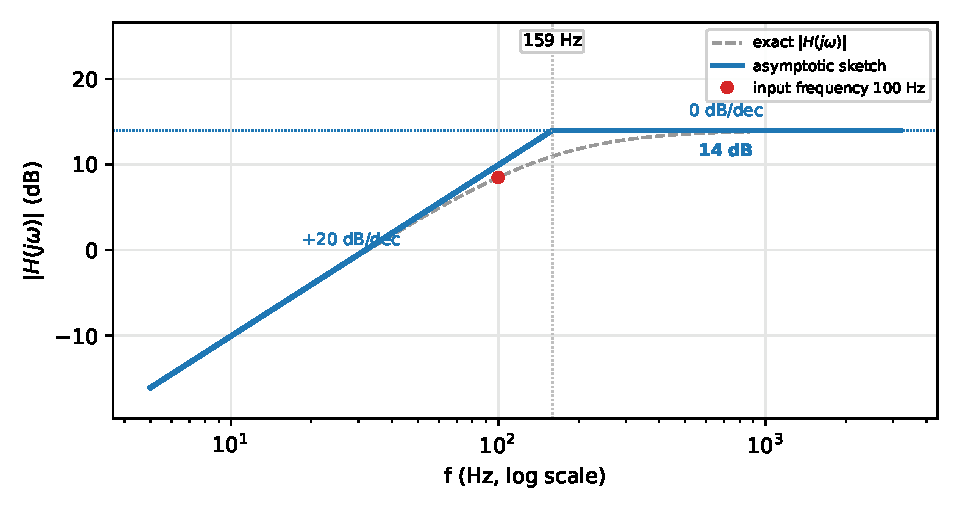
\includegraphics[width=0.78\linewidth,height=6.5cm,keepaspectratio]{p04_bode}\end{center}

{\small Blue: the straight-line sketch you are expected to draw. Dashed grey: the exact curve (about 3\,dB below the corner of an isolated pole). Red dot: the input frequency of Step 7.}
\solstep{7}{Steady-state output}The input is $V_i(t) = 0.2\sin\left(2\pi\cdot 100\,t\right)$, so $\omega_{in} = 2\pi\cdot 100 = 628$\,rad/s. Put $s=j\omega_{in}$ in each factor (tool T5): magnitudes multiply, angles add.
{\small Rules: $\left|\frac{s}{s+p}\right| = \frac{\omega}{\sqrt{\omega^2+p^2}}$, $\angle = \frac{\pi}{2}-\tan^{-1}\frac{\omega}{p}$;\quad $\left|\frac{1}{1+s/p}\right| = \frac{1}{\sqrt{1+(\omega/p)^2}}$, $\angle = -\tan^{-1}\frac{\omega}{p}$;\quad $\left|1+\frac{s}{z}\right| = \sqrt{1+(\omega/z)^2}$, $\angle = \tan^{-1}\frac{\omega}{z}$;\quad a negative $K$ adds $-\pi$.}
\begin{center}\renewcommand{\arraystretch}{1.35}
\begin{tabular}{ccc}
\toprule
factor & magnitude & angle (rad) \\
\midrule
$5$ & $5$ & $0$ \\
$\rule[-1.1em]{0pt}{2.8em}\dfrac{s}{s+2\pi\cdot 159}$ & $0.532$ & $1.01$ \\
\textbf{total} & $\mathbf{2.66}$ (product) & $\mathbf{1.01}$ (sum) \\
\bottomrule
\end{tabular}\end{center}

\begin{align*}
|H(j\omega_{in})| &= 2.66, \qquad \angle H(j\omega_{in}) = 1.01\ \mathrm{rad} \\
v_{o,ac}(t) &= 2.66\times 0.2\,\sin\left(2\pi\cdot 100\,t + 1.01\right) = 0.532\,\sin\left(2\pi\cdot 100\,t + 1.01\right)
\end{align*}

\[
\boxed{V_o(t) = 0.532\,\sin\left(2\pi\cdot 100\,t + 1.01\right)\ \mathrm{V}}
\]

\begin{ansbox}
$H(s) = 5\,\dfrac{s}{s+2\pi\cdot 159}$\quad (corners: 159 Hz)\\[4pt]
$V_o(t) = 0.532\,\sin\left(2\pi\cdot 100\,t + 1.01\right)\ \mathrm{V}$
\end{ansbox}

\newpage
\subsection*{Solution 2A.5 \hfill Easy}
\begin{center}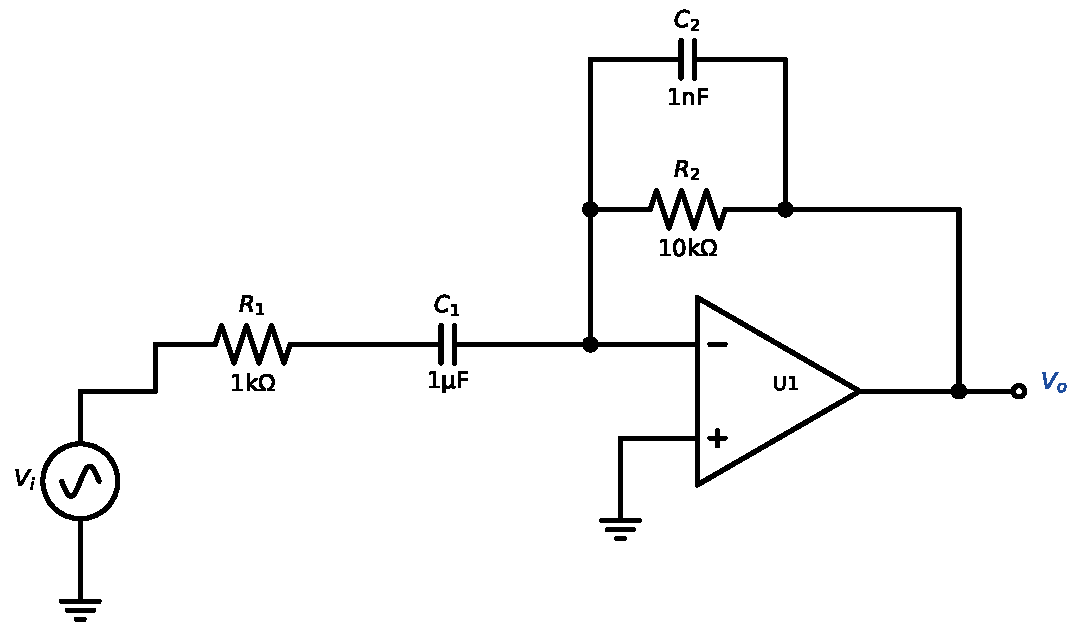
\includegraphics[width=\linewidth,height=5cm,keepaspectratio]{p05_circuit}\end{center}
\solstep{1}{Identify the sources}Independent sources: the AC input $V_i(t)$. No DC source: $V_{o,dc}=0$ and Step 2 is skipped.
\solstep{2}{DC circuit}No DC sources: $V_{o,dc}=0$.
\solstep{3}{Op-amp rules}The op-amp has negative feedback (its output is connected back to its $-$ input), so with an ideal op-amp (tool T1): (a) no current flows into the $+$ or $-$ input; (b) $V_-=V_+$ (virtual short). The circuit is a standard block, so use its block formula (tool T2).
\solstep{4}{Transfer function, block by block}\textbf{Block 1 (U1).} Inverting block: the $+$ input is grounded, so $V_- = V_+ = 0$ (virtual ground). The current $\frac{V_{i} - 0}{Z_{in1}}$ through $Z_{in1}$ cannot enter the op-amp, so all of it flows through $Z_{f1}$: $V_{o} = 0 - Z_{f1}\cdot\frac{V_{i}}{Z_{in1}}$.\begin{align*}
Z_{in1} &= R_{1} + \frac{1}{sC_{1}} = \dfrac{1000\,s + 10^{6}}{s} \\
Z_{f1} &= R_{2} \parallel \frac{1}{sC_{2}} = \dfrac{10^{9}}{s + 10^{5}}
\end{align*}
\[
\frac{V_{o}}{V_{i}} = -\frac{Z_{f1}}{Z_{in1}} = \dfrac{-10^{6}\,s}{s^{2} + 1.01\times 10^{5}\,s + 10^{8}}
\]

So:\[
H(s) = \dfrac{-10^{6}\,s}{s^{2} + 1.01\times 10^{5}\,s + 10^{8}}
\]

\solstep{5}{Standard (Bode-ready) form}Find the roots. Every root $s=-p$ of the denominator is a \emph{pole}, every root $s=-z$ of the numerator is a \emph{zero}; $|p|$ and $|z|$ are the corner frequencies (rad/s).
\begin{itemize}[leftmargin=*,itemsep=2pt]
\item Numerator: it has the factor $s$ $\Rightarrow$ 1 zero at $s=0$.
\item Denominator: $s^{2} + 1.01\times 10^{5}\,s + 10^{8}$; quadratic formula:\[
s = \frac{-1.01\times 10^{5} \pm \sqrt{(1.01\times 10^{5})^2 - 4(10^{8})}}{2} = \frac{-1.01\times 10^{5} \pm 99000}{2} \Rightarrow s = -1000,\ -10^{5}
\]

\end{itemize}

Factored form (leading coefficient in front):
\[
H(s) = -10^{6}\,\dfrac{s}{(s+1000)(s+10^{5})}
\]

Bode-ready form: rewrite every $(s+p) = p\left(1+\frac{s}{p}\right)$ and $(s+z) = z\left(1+\frac{s}{z}\right)$, and collect all constants into $K$. Each $s$ in the numerator is paired with one of the \emph{lowest} poles as $\frac{s}{s+p}$ (that factor is $\approx 1$ above $p$). Then every factor except $K$ is $\approx 1$ inside the pass-band:
\[
H(s) = -10\,\dfrac{s}{s+2\pi\cdot 159}\,\dfrac{1}{1+\dfrac{s}{2\pi\cdot 15.9\mathrm{k}}},\qquad K = -10
\]

\begin{center}\renewcommand{\arraystretch}{1.35}
\begin{tabular}{cccc}
\toprule
type & $\omega_c$ (rad/s) & $f_c=\omega_c/2\pi$ & slope change \\
\midrule
pole & $1000$ & 159 Hz & $-20$ dB/dec \\
pole & $10^{5}$ & 15.9 kHz & $-20$ dB/dec \\
\bottomrule
\end{tabular}\end{center}

\solstep{6}{Magnitude Bode plot}Below every corner $|H(s)|\approx 0.01\,s$, so the plot starts with a slope of $+20$\,dB/dec. Then, moving right, each pole bends the line down by 20\,dB/dec and each zero bends it up by 20\,dB/dec (tool T6):
\begin{center}\renewcommand{\arraystretch}{1.35}
\begin{tabular}{lcl}
\toprule
frequency range & slope & asymptote level \\
\midrule
$f<$ 159 Hz & $+20$ dB/dec & 20 dB at end \\
159 Hz -- 15.9 kHz & $0$ dB/dec (flat) & 20 dB at start, 20 dB at end \\
$f>$ 15.9 kHz & $-20$ dB/dec & 20 dB at start \\
\bottomrule
\end{tabular}\end{center}

The flat (pass-band) level is $20\log_{10}|K| = 20\log_{10}10 = 20$\,dB.
\begin{center}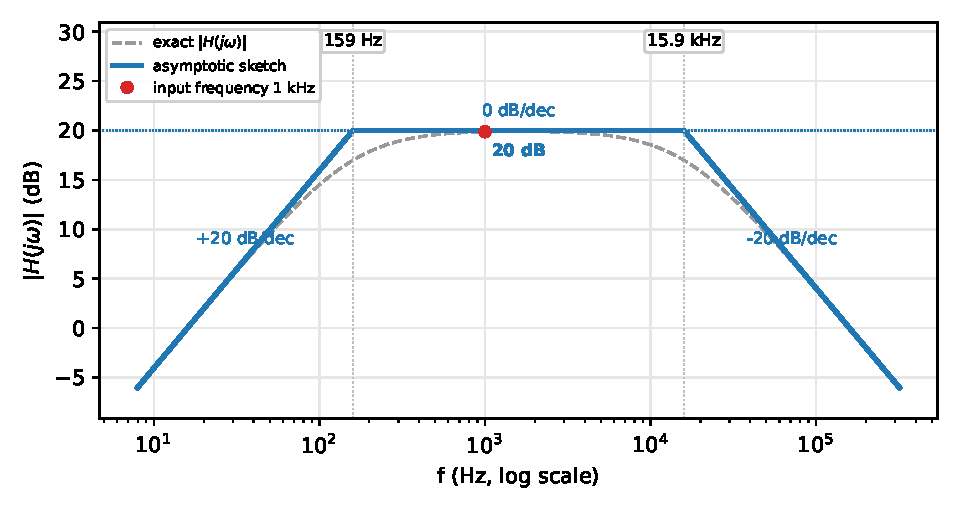
\includegraphics[width=0.78\linewidth,height=6.5cm,keepaspectratio]{p05_bode}\end{center}

{\small Blue: the straight-line sketch you are expected to draw. Dashed grey: the exact curve (about 3\,dB below the corner of an isolated pole). Red dot: the input frequency of Step 7.}
\solstep{7}{Steady-state output}The input is $V_i(t) = 0.05\sin\left(2\pi\cdot 1000\,t\right)$, so $\omega_{in} = 2\pi\cdot 1000 = 6280$\,rad/s. Put $s=j\omega_{in}$ in each factor (tool T5): magnitudes multiply, angles add.
{\small Rules: $\left|\frac{s}{s+p}\right| = \frac{\omega}{\sqrt{\omega^2+p^2}}$, $\angle = \frac{\pi}{2}-\tan^{-1}\frac{\omega}{p}$;\quad $\left|\frac{1}{1+s/p}\right| = \frac{1}{\sqrt{1+(\omega/p)^2}}$, $\angle = -\tan^{-1}\frac{\omega}{p}$;\quad $\left|1+\frac{s}{z}\right| = \sqrt{1+(\omega/z)^2}$, $\angle = \tan^{-1}\frac{\omega}{z}$;\quad a negative $K$ adds $-\pi$.}
\begin{center}\renewcommand{\arraystretch}{1.35}
\begin{tabular}{ccc}
\toprule
factor & magnitude & angle (rad) \\
\midrule
$-10$ & $10$ & $-3.14$ \\
$\rule[-1.1em]{0pt}{2.8em}\dfrac{s}{s+2\pi\cdot 159}$ & $0.9876$ & $0.158$ \\
$\rule[-1.7em]{0pt}{4em}\dfrac{1}{1+\dfrac{s}{2\pi\cdot 15.9\mathrm{k}}}$ & $0.998$ & $-0.0627$ \\
\textbf{total} & $\mathbf{9.856}$ (product) & $\mathbf{-3.05}$ (sum) \\
\bottomrule
\end{tabular}\end{center}

\begin{align*}
|H(j\omega_{in})| &= 9.86, \qquad \angle H(j\omega_{in}) = -3.05\ \mathrm{rad} \\
v_{o,ac}(t) &= 9.86\times 0.05\,\sin\left(2\pi\cdot 1000\,t - 3.05\right) = 0.493\,\sin\left(2\pi\cdot 1000\,t - 3.05\right)
\end{align*}

\[
\boxed{V_o(t) = 0.493\,\sin\left(2\pi\cdot 1000\,t - 3.05\right)\ \mathrm{V}}
\]

\begin{ansbox}
$H(s) = -10\,\dfrac{s}{s+2\pi\cdot 159}\,\dfrac{1}{1+\dfrac{s}{2\pi\cdot 15.9\mathrm{k}}}$\quad (corners: 159 Hz, 15.9 kHz)\\[4pt]
$V_o(t) = 0.493\,\sin\left(2\pi\cdot 1000\,t - 3.05\right)\ \mathrm{V}$
\end{ansbox}

\newpage
\subsection*{Solution 2A.6 \hfill Easy}
\begin{center}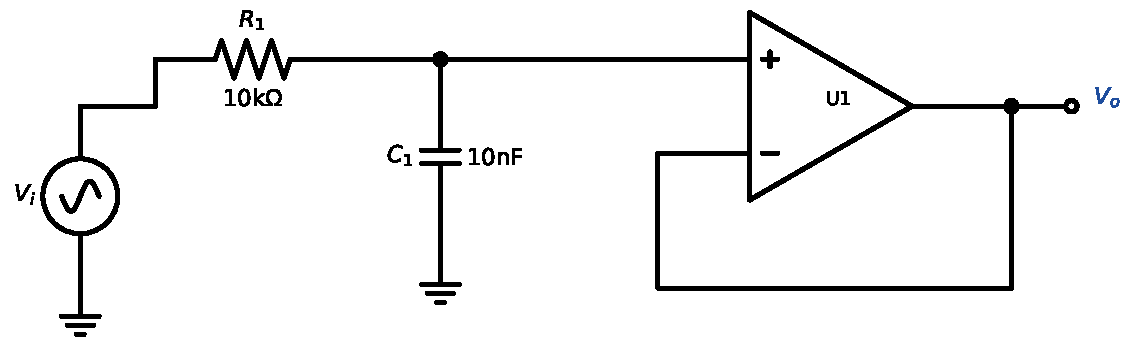
\includegraphics[width=\linewidth,height=5cm,keepaspectratio]{p06_circuit}\end{center}
\solstep{1}{Identify the sources}Independent sources: the AC input $V_i(t)$. No DC source: $V_{o,dc}=0$ and Step 2 is skipped.
\solstep{2}{DC circuit}No DC sources: $V_{o,dc}=0$.
\solstep{3}{Op-amp rules}The op-amp has negative feedback (its output is connected back to its $-$ input), so with an ideal op-amp (tool T1): (a) no current flows into the $+$ or $-$ input; (b) $V_-=V_+$ (virtual short). The circuit is a standard block, so use its block formula (tool T2).
\solstep{4}{Transfer function, block by block}\textbf{Block 1 (U1).} Non-inverting block: No current flows into the $+$ input, so $\frac{1}{sC_{1}}$ and $R_{1}$ form a plain voltage divider: $V_+ = \frac{\frac{1}{sC_{1}}}{R_{1} + \frac{1}{sC_{1}}}V_{i}$. The output is tied back to the $-$ input, so $V_{o} = V_- = V_+$ (voltage follower).\[
\frac{V_{o}}{V_{i}} = \frac{\frac{1}{sC_{1}}}{R_{1} + \frac{1}{sC_{1}}} = \dfrac{10000}{s + 10000}
\]

So:\[
H(s) = \dfrac{10000}{s + 10000}
\]

\solstep{5}{Standard (Bode-ready) form}Find the roots. Every root $s=-p$ of the denominator is a \emph{pole}, every root $s=-z$ of the numerator is a \emph{zero}; $|p|$ and $|z|$ are the corner frequencies (rad/s).
\begin{itemize}[leftmargin=*,itemsep=2pt]
\item Denominator: $s + 10000$; $s + 10000 = 0 \Rightarrow s = -10000$.
\end{itemize}

Factored form (leading coefficient in front):
\[
H(s) = 10000\,\dfrac{1}{(s+10000)}
\]

Bode-ready form: rewrite every $(s+p) = p\left(1+\frac{s}{p}\right)$ and $(s+z) = z\left(1+\frac{s}{z}\right)$, and collect all constants into $K$. Then every factor except $K$ is $\approx 1$ inside the pass-band:
\[
H(s) = 1\,\dfrac{1}{1+\dfrac{s}{2\pi\cdot 1.59\mathrm{k}}},\qquad K = 1
\]

\begin{center}\renewcommand{\arraystretch}{1.35}
\begin{tabular}{cccc}
\toprule
type & $\omega_c$ (rad/s) & $f_c=\omega_c/2\pi$ & slope change \\
\midrule
pole & $10000$ & 1.59 kHz & $-20$ dB/dec \\
\bottomrule
\end{tabular}\end{center}

\solstep{6}{Magnitude Bode plot}Below every corner, all factors are $\approx$ constant: $|H| \approx 1$ $= 0$\,dB (flat, 0 dB/dec). Then, moving right, each pole bends the line down by 20\,dB/dec and each zero bends it up by 20\,dB/dec (tool T6):
\begin{center}\renewcommand{\arraystretch}{1.35}
\begin{tabular}{lcl}
\toprule
frequency range & slope & asymptote level \\
\midrule
$f<$ 1.59 kHz & $0$ dB/dec (flat) & 0 dB at end \\
$f>$ 1.59 kHz & $-20$ dB/dec & 0 dB at start \\
\bottomrule
\end{tabular}\end{center}

The flat (pass-band) level is $20\log_{10}|K| = 20\log_{10}1 = 0$\,dB.
\begin{center}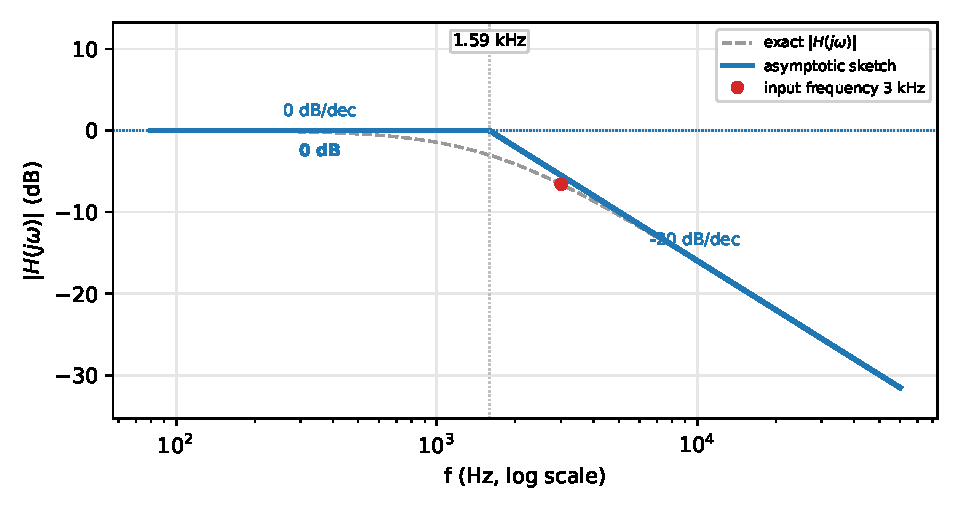
\includegraphics[width=0.78\linewidth,height=6.5cm,keepaspectratio]{p06_bode}\end{center}

{\small Blue: the straight-line sketch you are expected to draw. Dashed grey: the exact curve (about 3\,dB below the corner of an isolated pole). Red dot: the input frequency of Step 7.}
\solstep{7}{Steady-state output}The input is $V_i(t) = 1\cos\left(2\pi\cdot 3000\,t\right)$, so $\omega_{in} = 2\pi\cdot 3000 = 18800$\,rad/s. Put $s=j\omega_{in}$ in each factor (tool T5): magnitudes multiply, angles add.
{\small Rules: $\left|\frac{s}{s+p}\right| = \frac{\omega}{\sqrt{\omega^2+p^2}}$, $\angle = \frac{\pi}{2}-\tan^{-1}\frac{\omega}{p}$;\quad $\left|\frac{1}{1+s/p}\right| = \frac{1}{\sqrt{1+(\omega/p)^2}}$, $\angle = -\tan^{-1}\frac{\omega}{p}$;\quad $\left|1+\frac{s}{z}\right| = \sqrt{1+(\omega/z)^2}$, $\angle = \tan^{-1}\frac{\omega}{z}$;\quad a negative $K$ adds $-\pi$.}
\begin{center}\renewcommand{\arraystretch}{1.35}
\begin{tabular}{ccc}
\toprule
factor & magnitude & angle (rad) \\
\midrule
$1$ & $1$ & $0$ \\
$\rule[-1.7em]{0pt}{4em}\dfrac{1}{1+\dfrac{s}{2\pi\cdot 1.59\mathrm{k}}}$ & $0.4686$ & $-1.08$ \\
\textbf{total} & $\mathbf{0.4686}$ (product) & $\mathbf{-1.08}$ (sum) \\
\bottomrule
\end{tabular}\end{center}

\begin{align*}
|H(j\omega_{in})| &= 0.469, \qquad \angle H(j\omega_{in}) = -1.08\ \mathrm{rad} \\
v_{o,ac}(t) &= 0.469\times 1\,\cos\left(2\pi\cdot 3000\,t - 1.08\right) = 0.469\,\cos\left(2\pi\cdot 3000\,t - 1.08\right)
\end{align*}

\[
\boxed{V_o(t) = 0.469\,\cos\left(2\pi\cdot 3000\,t - 1.08\right)\ \mathrm{V}}
\]

\begin{ansbox}
$H(s) = 1\,\dfrac{1}{1+\dfrac{s}{2\pi\cdot 1.59\mathrm{k}}}$\quad (corners: 1.59 kHz)\\[4pt]
$V_o(t) = 0.469\,\cos\left(2\pi\cdot 3000\,t - 1.08\right)\ \mathrm{V}$
\end{ansbox}

\newpage
\subsection*{Solution 2A.7 \hfill Medium}
\begin{center}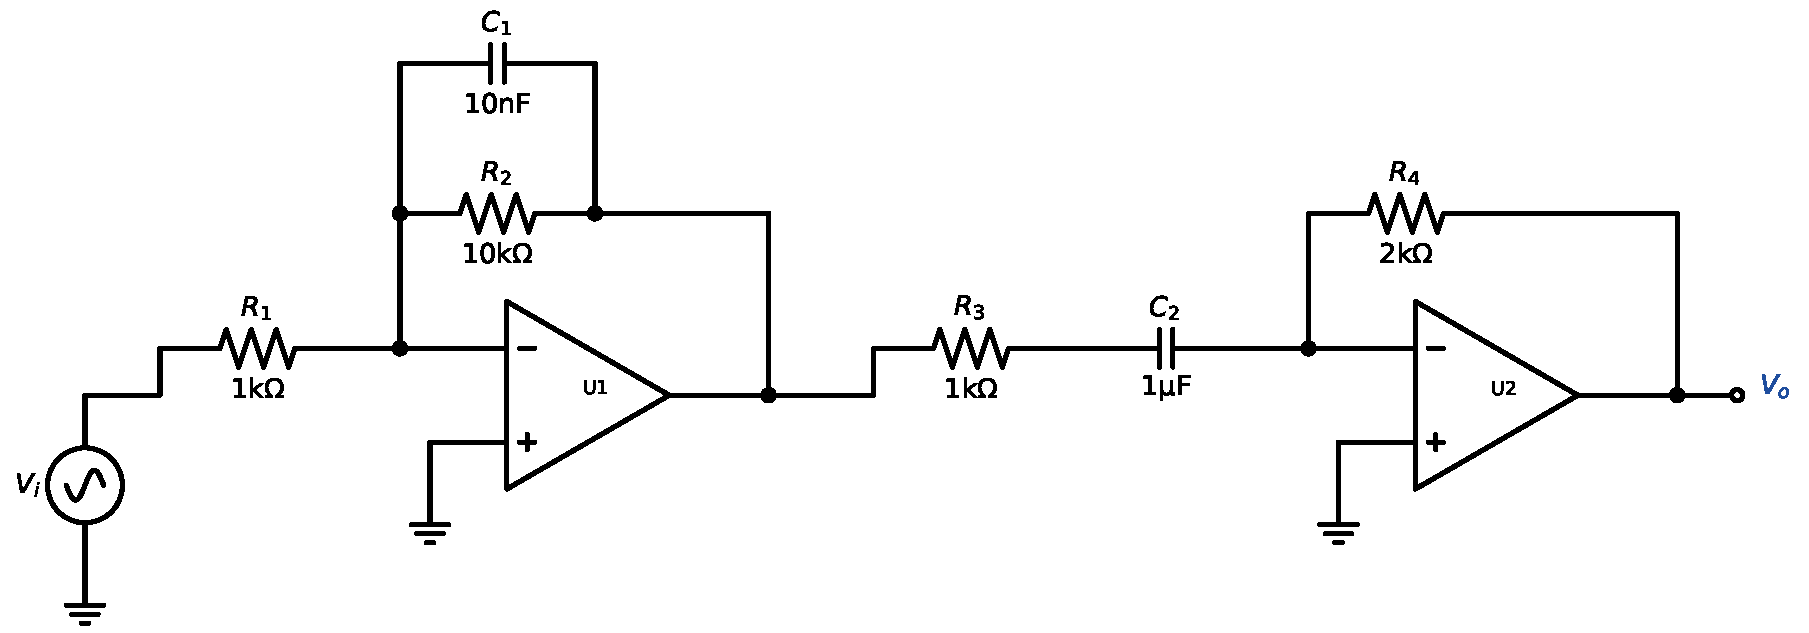
\includegraphics[width=\linewidth,height=5cm,keepaspectratio]{p07_circuit}\end{center}
\solstep{1}{Identify the sources}Independent sources: the AC input $V_i(t)$. No DC source: $V_{o,dc}=0$ and Step 2 is skipped.
\solstep{2}{DC circuit}No DC sources: $V_{o,dc}=0$.
\solstep{3}{Op-amp rules}Each op-amp has negative feedback (its output is connected back to its $-$ input), so with an ideal op-amp (tool T1): (a) no current flows into the $+$ or $-$ input; (b) $V_-=V_+$ (virtual short). The circuit is a cascade of standard blocks, so each block is solved with its block formula (tool T2).
\solstep{4}{Transfer function, block by block}Each op-amp output is an ideal voltage source, so a block's output does not change when the next block is connected: the blocks can be solved one at a time and multiplied.\[
H(s) = \frac{V_o}{V_i} = \frac{V_{o1}}{V_{i}}\cdot\frac{V_{o}}{V_{o1}}
\]

\textbf{Block 1 (U1).} Inverting block: the $+$ input is grounded, so $V_- = V_+ = 0$ (virtual ground). The current $\frac{V_{i} - 0}{R_{1}}$ through $R_{1}$ cannot enter the op-amp, so all of it flows through $Z_{f1}$: $V_{o1} = 0 - Z_{f1}\cdot\frac{V_{i}}{R_{1}}$.\begin{align*}
Z_{f1} &= R_{2} \parallel \frac{1}{sC_{1}} = \dfrac{10^{8}}{s + 10000}
\end{align*}
\[
\frac{V_{o1}}{V_{i}} = -\frac{Z_{f1}}{R_{1}} = \dfrac{-10^{5}}{s + 10000}
\]

\textbf{Block 2 (U2).} Inverting block: the $+$ input is grounded, so $V_- = V_+ = 0$ (virtual ground). The current $\frac{V_{o1} - 0}{Z_{in2}}$ through $Z_{in2}$ cannot enter the op-amp, so all of it flows through $R_{4}$: $V_{o} = 0 - R_{4}\cdot\frac{V_{o1}}{Z_{in2}}$.\begin{align*}
Z_{in2} &= R_{3} + \frac{1}{sC_{2}} = \dfrac{1000\,s + 10^{6}}{s}
\end{align*}
\[
\frac{V_{o}}{V_{o1}} = -\frac{R_{4}}{Z_{in2}} = \dfrac{-2\,s}{s + 1000}
\]

Multiply the blocks and simplify:\[
H(s) = \dfrac{2\times 10^{5}\,s}{s^{2} + 11000\,s + 10^{7}}
\]

\solstep{5}{Standard (Bode-ready) form}Find the roots. Every root $s=-p$ of the denominator is a \emph{pole}, every root $s=-z$ of the numerator is a \emph{zero}; $|p|$ and $|z|$ are the corner frequencies (rad/s).
\begin{itemize}[leftmargin=*,itemsep=2pt]
\item Numerator: it has the factor $s$ $\Rightarrow$ 1 zero at $s=0$.
\item Denominator: $s^{2} + 11000\,s + 10^{7}$; quadratic formula:\[
s = \frac{-11000 \pm \sqrt{(11000)^2 - 4(10^{7})}}{2} = \frac{-11000 \pm 9000}{2} \Rightarrow s = -1000,\ -10000
\]

\end{itemize}

Factored form (leading coefficient in front):
\[
H(s) = 2\times 10^{5}\,\dfrac{s}{(s+1000)(s+10000)}
\]

Bode-ready form: rewrite every $(s+p) = p\left(1+\frac{s}{p}\right)$ and $(s+z) = z\left(1+\frac{s}{z}\right)$, and collect all constants into $K$. Each $s$ in the numerator is paired with one of the \emph{lowest} poles as $\frac{s}{s+p}$ (that factor is $\approx 1$ above $p$). Then every factor except $K$ is $\approx 1$ inside the pass-band:
\[
H(s) = 20\,\dfrac{s}{s+2\pi\cdot 159}\,\dfrac{1}{1+\dfrac{s}{2\pi\cdot 1.59\mathrm{k}}},\qquad K = 20
\]

\begin{center}\renewcommand{\arraystretch}{1.35}
\begin{tabular}{cccc}
\toprule
type & $\omega_c$ (rad/s) & $f_c=\omega_c/2\pi$ & slope change \\
\midrule
pole & $1000$ & 159 Hz & $-20$ dB/dec \\
pole & $10000$ & 1.59 kHz & $-20$ dB/dec \\
\bottomrule
\end{tabular}\end{center}

\solstep{6}{Magnitude Bode plot}Below every corner $|H(s)|\approx 0.02\,s$, so the plot starts with a slope of $+20$\,dB/dec. Then, moving right, each pole bends the line down by 20\,dB/dec and each zero bends it up by 20\,dB/dec (tool T6):
\begin{center}\renewcommand{\arraystretch}{1.35}
\begin{tabular}{lcl}
\toprule
frequency range & slope & asymptote level \\
\midrule
$f<$ 159 Hz & $+20$ dB/dec & 26 dB at end \\
159 Hz -- 1.59 kHz & $0$ dB/dec (flat) & 26 dB at start, 26 dB at end \\
$f>$ 1.59 kHz & $-20$ dB/dec & 26 dB at start \\
\bottomrule
\end{tabular}\end{center}

The flat (pass-band) level is $20\log_{10}|K| = 20\log_{10}20 = 26$\,dB.
\begin{center}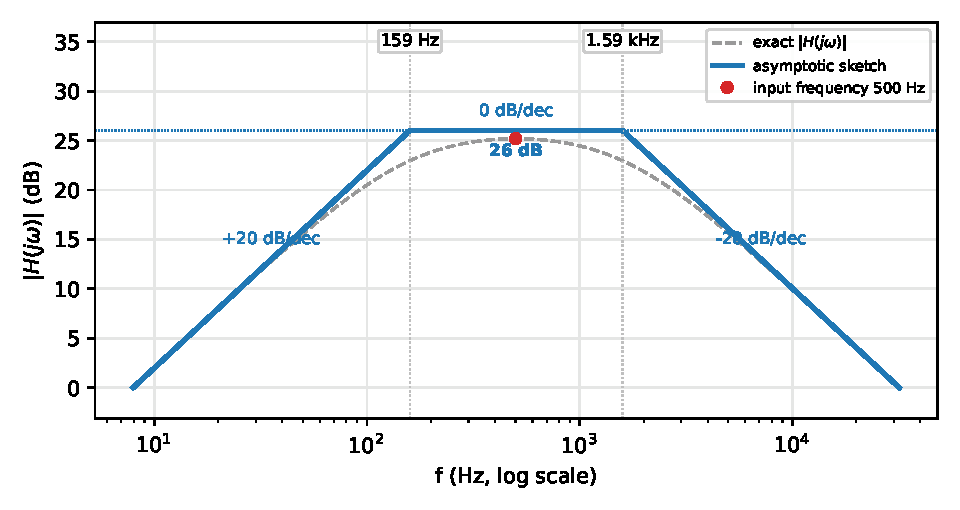
\includegraphics[width=0.78\linewidth,height=6.5cm,keepaspectratio]{p07_bode}\end{center}

{\small Blue: the straight-line sketch you are expected to draw. Dashed grey: the exact curve (about 3\,dB below the corner of an isolated pole). Red dot: the input frequency of Step 7.}
\solstep{7}{Steady-state output}The input is $V_i(t) = 0.02\sin\left(2\pi\cdot 500\,t\right)$, so $\omega_{in} = 2\pi\cdot 500 = 3140$\,rad/s. Put $s=j\omega_{in}$ in each factor (tool T5): magnitudes multiply, angles add.
{\small Rules: $\left|\frac{s}{s+p}\right| = \frac{\omega}{\sqrt{\omega^2+p^2}}$, $\angle = \frac{\pi}{2}-\tan^{-1}\frac{\omega}{p}$;\quad $\left|\frac{1}{1+s/p}\right| = \frac{1}{\sqrt{1+(\omega/p)^2}}$, $\angle = -\tan^{-1}\frac{\omega}{p}$;\quad $\left|1+\frac{s}{z}\right| = \sqrt{1+(\omega/z)^2}$, $\angle = \tan^{-1}\frac{\omega}{z}$;\quad a negative $K$ adds $-\pi$.}
\begin{center}\renewcommand{\arraystretch}{1.35}
\begin{tabular}{ccc}
\toprule
factor & magnitude & angle (rad) \\
\midrule
$20$ & $20$ & $0$ \\
$\rule[-1.1em]{0pt}{2.8em}\dfrac{s}{s+2\pi\cdot 159}$ & $0.9529$ & $0.308$ \\
$\rule[-1.7em]{0pt}{4em}\dfrac{1}{1+\dfrac{s}{2\pi\cdot 1.59\mathrm{k}}}$ & $0.954$ & $-0.304$ \\
\textbf{total} & $\mathbf{18.18}$ (product) & $\mathbf{0.00377}$ (sum) \\
\bottomrule
\end{tabular}\end{center}

\begin{align*}
|H(j\omega_{in})| &= 18.2, \qquad \angle H(j\omega_{in}) = 0.00377\ \mathrm{rad} \\
v_{o,ac}(t) &= 18.2\times 0.02\,\sin\left(2\pi\cdot 500\,t + 0.00377\right) = 0.364\,\sin\left(2\pi\cdot 500\,t + 0.00377\right)
\end{align*}

\[
\boxed{V_o(t) = 0.364\,\sin\left(2\pi\cdot 500\,t + 0.00377\right)\ \mathrm{V}}
\]

\begin{ansbox}
$H(s) = 20\,\dfrac{s}{s+2\pi\cdot 159}\,\dfrac{1}{1+\dfrac{s}{2\pi\cdot 1.59\mathrm{k}}}$\quad (corners: 159 Hz, 1.59 kHz)\\[4pt]
$V_o(t) = 0.364\,\sin\left(2\pi\cdot 500\,t + 0.00377\right)\ \mathrm{V}$
\end{ansbox}

\newpage
\subsection*{Solution 2A.8 \hfill Medium}
\begin{center}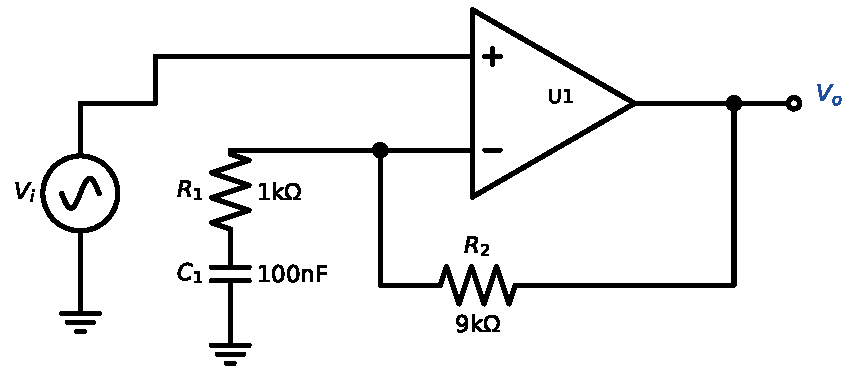
\includegraphics[width=\linewidth,height=5cm,keepaspectratio]{p08_circuit}\end{center}
\solstep{1}{Identify the sources}Independent sources: the AC input $V_i(t)$. No DC source: $V_{o,dc}=0$ and Step 2 is skipped.
\solstep{2}{DC circuit}No DC sources: $V_{o,dc}=0$.
\solstep{3}{Op-amp rules}The op-amp has negative feedback (its output is connected back to its $-$ input), so with an ideal op-amp (tool T1): (a) no current flows into the $+$ or $-$ input; (b) $V_-=V_+$ (virtual short). The circuit is a standard block, so use its block formula (tool T2).
\solstep{4}{Transfer function, block by block}\textbf{Block 1 (U1).} Non-inverting block: The $+$ input is the block input: $V_+ = V_{i}$. The op-amp forces $V_-=V_+$, and $Z_{g1}$, $R_{2}$ divide the output: $V_- = \frac{Z_{g1}}{Z_{g1} + R_{2}}V_{o}$, hence $V_{o} = \left(1+\frac{R_{2}}{Z_{g1}}\right)V_+$.\begin{align*}
Z_{g1} &= R_{1} + \frac{1}{sC_{1}} = \dfrac{1000\,s + 10^{7}}{s}
\end{align*}
\[
\frac{V_{o}}{V_{i}} = \left(1+\frac{R_{2}}{Z_{g1}}\right) = \dfrac{10\,s + 10000}{s + 10000}
\]

So:\[
H(s) = \dfrac{10\,s + 10000}{s + 10000}
\]

\solstep{5}{Standard (Bode-ready) form}Find the roots. Every root $s=-p$ of the denominator is a \emph{pole}, every root $s=-z$ of the numerator is a \emph{zero}; $|p|$ and $|z|$ are the corner frequencies (rad/s).
\begin{itemize}[leftmargin=*,itemsep=2pt]
\item Numerator: $10\,s + 10000$; divide by the leading coefficient $10$ (this does not move the roots): $s + 1000$; $s + 1000 = 0 \Rightarrow s = -1000$.
\item Denominator: $s + 10000$; $s + 10000 = 0 \Rightarrow s = -10000$.
\end{itemize}

Factored form (leading coefficient in front):
\[
H(s) = 10\,\dfrac{(s+1000)}{(s+10000)}
\]

Bode-ready form: rewrite every $(s+p) = p\left(1+\frac{s}{p}\right)$ and $(s+z) = z\left(1+\frac{s}{z}\right)$, and collect all constants into $K$. Then every factor except $K$ is $\approx 1$ inside the pass-band:
\[
H(s) = 1\,\left(1+\dfrac{s}{2\pi\cdot 159}\right)\,\dfrac{1}{1+\dfrac{s}{2\pi\cdot 1.59\mathrm{k}}},\qquad K = 1
\]

\begin{center}\renewcommand{\arraystretch}{1.35}
\begin{tabular}{cccc}
\toprule
type & $\omega_c$ (rad/s) & $f_c=\omega_c/2\pi$ & slope change \\
\midrule
zero & $1000$ & 159 Hz & $+20$ dB/dec \\
pole & $10000$ & 1.59 kHz & $-20$ dB/dec \\
\bottomrule
\end{tabular}\end{center}

\solstep{6}{Magnitude Bode plot}Below every corner, all factors are $\approx$ constant: $|H| \approx 1$ $= 0$\,dB (flat, 0 dB/dec). Then, moving right, each pole bends the line down by 20\,dB/dec and each zero bends it up by 20\,dB/dec (tool T6):
\begin{center}\renewcommand{\arraystretch}{1.35}
\begin{tabular}{lcl}
\toprule
frequency range & slope & asymptote level \\
\midrule
$f<$ 159 Hz & $0$ dB/dec (flat) & 0 dB at end \\
159 Hz -- 1.59 kHz & $+20$ dB/dec & 0 dB at start, 20 dB at end \\
$f>$ 1.59 kHz & $0$ dB/dec (flat) & 20 dB at start \\
\bottomrule
\end{tabular}\end{center}

\begin{center}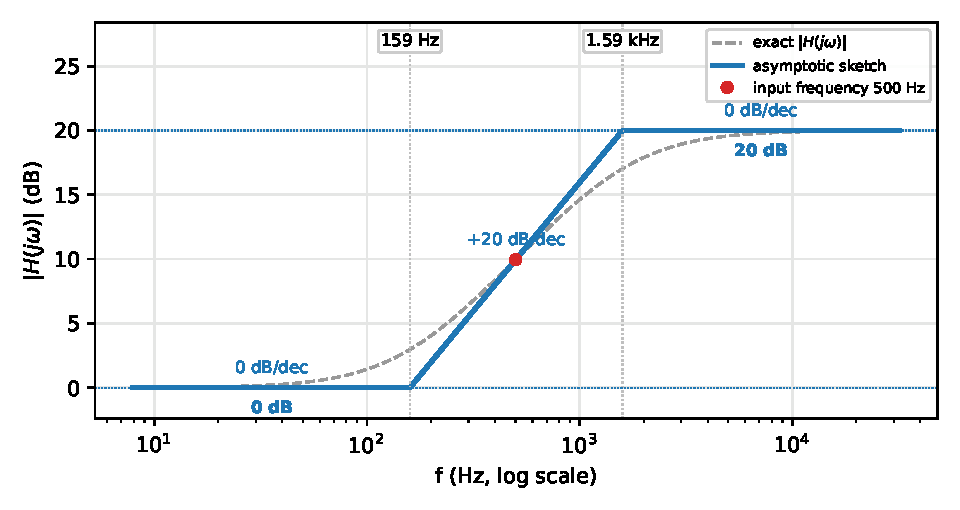
\includegraphics[width=0.78\linewidth,height=6.5cm,keepaspectratio]{p08_bode}\end{center}

{\small Blue: the straight-line sketch you are expected to draw. Dashed grey: the exact curve (about 3\,dB below the corner of an isolated pole). Red dot: the input frequency of Step 7.}
\solstep{7}{Steady-state output}The input is $V_i(t) = 0.1\sin\left(2\pi\cdot 500\,t\right)$, so $\omega_{in} = 2\pi\cdot 500 = 3140$\,rad/s. Put $s=j\omega_{in}$ in each factor (tool T5): magnitudes multiply, angles add.
{\small Rules: $\left|\frac{s}{s+p}\right| = \frac{\omega}{\sqrt{\omega^2+p^2}}$, $\angle = \frac{\pi}{2}-\tan^{-1}\frac{\omega}{p}$;\quad $\left|\frac{1}{1+s/p}\right| = \frac{1}{\sqrt{1+(\omega/p)^2}}$, $\angle = -\tan^{-1}\frac{\omega}{p}$;\quad $\left|1+\frac{s}{z}\right| = \sqrt{1+(\omega/z)^2}$, $\angle = \tan^{-1}\frac{\omega}{z}$;\quad a negative $K$ adds $-\pi$.}
\begin{center}\renewcommand{\arraystretch}{1.35}
\begin{tabular}{ccc}
\toprule
factor & magnitude & angle (rad) \\
\midrule
$1$ & $1$ & $0$ \\
$\rule[-1.1em]{0pt}{2.8em}\left(1+\dfrac{s}{2\pi\cdot 159}\right)$ & $3.297$ & $1.26$ \\
$\rule[-1.7em]{0pt}{4em}\dfrac{1}{1+\dfrac{s}{2\pi\cdot 1.59\mathrm{k}}}$ & $0.954$ & $-0.304$ \\
\textbf{total} & $\mathbf{3.145}$ (product) & $\mathbf{0.958}$ (sum) \\
\bottomrule
\end{tabular}\end{center}

\begin{align*}
|H(j\omega_{in})| &= 3.15, \qquad \angle H(j\omega_{in}) = 0.958\ \mathrm{rad} \\
v_{o,ac}(t) &= 3.15\times 0.1\,\sin\left(2\pi\cdot 500\,t + 0.958\right) = 0.315\,\sin\left(2\pi\cdot 500\,t + 0.958\right)
\end{align*}

\[
\boxed{V_o(t) = 0.315\,\sin\left(2\pi\cdot 500\,t + 0.958\right)\ \mathrm{V}}
\]

\begin{ansbox}
$H(s) = 1\,\left(1+\dfrac{s}{2\pi\cdot 159}\right)\,\dfrac{1}{1+\dfrac{s}{2\pi\cdot 1.59\mathrm{k}}}$\quad (corners: 159 Hz, 1.59 kHz)\\[4pt]
$V_o(t) = 0.315\,\sin\left(2\pi\cdot 500\,t + 0.958\right)\ \mathrm{V}$
\end{ansbox}

\newpage
\subsection*{Solution 2A.9 \hfill Medium}
\begin{center}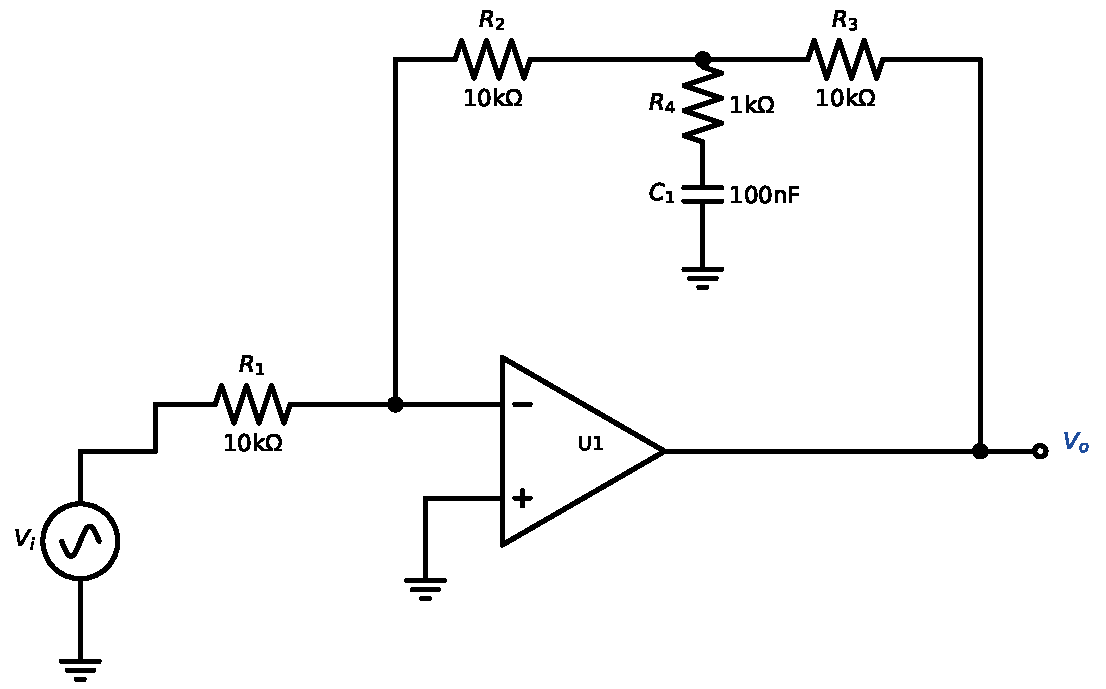
\includegraphics[width=\linewidth,height=5cm,keepaspectratio]{p09_circuit}\end{center}
\solstep{1}{Identify the sources}Independent sources: the AC input $V_i(t)$. No DC source: $V_{o,dc}=0$ and Step 2 is skipped.
\solstep{2}{DC circuit}No DC sources: $V_{o,dc}=0$.
\solstep{3}{Op-amp rules}The op-amp has negative feedback (its output is connected back to its $-$ input), so with an ideal op-amp (tool T1): (a) no current flows into the $+$ or $-$ input; (b) $V_-=V_+$ (virtual short). The circuit is a standard block, so use its block formula (tool T2).
\solstep{4}{Transfer function, block by block}\textbf{Block 1 (U1).} T-network block. Virtual ground: $V_-=0$, so $I = \frac{V_{i}}{R_{1}}$ flows through $R_{1}$ and (no current into the op-amp) on through $R_{2}$. The T node is at $V_T = 0 - R_{2}I$. $Z_{c1}$ takes $\frac{V_T}{Z_{c1}}$ to ground, so KCL at the T node leaves $I_b = I - \frac{V_T}{Z_{c1}} = I\left(1+\frac{R_{2}}{Z_{c1}}\right)$ for $R_{3}$. Then $V_{o} = V_T - R_{3}I_b = -\left(R_{2}+R_{3}+\frac{R_{2}R_{3}}{Z_{c1}}\right)I$.\begin{align*}
Z_{c1} &= R_{4} + \frac{1}{sC_{1}} = \dfrac{1000\,s + 10^{7}}{s}
\end{align*}
\[
\frac{V_{o}}{V_{i}} = -\frac{R_{2} + R_{3} + \frac{R_{2}\,R_{3}}{Z_{c1}}}{R_{1}} = \dfrac{-12\,s - 20000}{s + 10000}
\]

So:\[
H(s) = \dfrac{-12\,s - 20000}{s + 10000}
\]

\solstep{5}{Standard (Bode-ready) form}Find the roots. Every root $s=-p$ of the denominator is a \emph{pole}, every root $s=-z$ of the numerator is a \emph{zero}; $|p|$ and $|z|$ are the corner frequencies (rad/s).
\begin{itemize}[leftmargin=*,itemsep=2pt]
\item Numerator: $-12\,s - 20000$; divide by the leading coefficient $-12$ (this does not move the roots): $s + 1670$; $s + 1670 = 0 \Rightarrow s = -1670$.
\item Denominator: $s + 10000$; $s + 10000 = 0 \Rightarrow s = -10000$.
\end{itemize}

Factored form (leading coefficient in front):
\[
H(s) = -12\,\dfrac{(s+1670)}{(s+10000)}
\]

Bode-ready form: rewrite every $(s+p) = p\left(1+\frac{s}{p}\right)$ and $(s+z) = z\left(1+\frac{s}{z}\right)$, and collect all constants into $K$. Then every factor except $K$ is $\approx 1$ inside the pass-band:
\[
H(s) = -2\,\left(1+\dfrac{s}{2\pi\cdot 265}\right)\,\dfrac{1}{1+\dfrac{s}{2\pi\cdot 1.59\mathrm{k}}},\qquad K = -2
\]

\begin{center}\renewcommand{\arraystretch}{1.35}
\begin{tabular}{cccc}
\toprule
type & $\omega_c$ (rad/s) & $f_c=\omega_c/2\pi$ & slope change \\
\midrule
zero & $1670$ & 265 Hz & $+20$ dB/dec \\
pole & $10000$ & 1.59 kHz & $-20$ dB/dec \\
\bottomrule
\end{tabular}\end{center}

\solstep{6}{Magnitude Bode plot}Below every corner, all factors are $\approx$ constant: $|H| \approx 2$ $= 6.02$\,dB (flat, 0 dB/dec). Then, moving right, each pole bends the line down by 20\,dB/dec and each zero bends it up by 20\,dB/dec (tool T6):
\begin{center}\renewcommand{\arraystretch}{1.35}
\begin{tabular}{lcl}
\toprule
frequency range & slope & asymptote level \\
\midrule
$f<$ 265 Hz & $0$ dB/dec (flat) & 6.02 dB at end \\
265 Hz -- 1.59 kHz & $+20$ dB/dec & 6.02 dB at start, 21.6 dB at end \\
$f>$ 1.59 kHz & $0$ dB/dec (flat) & 21.6 dB at start \\
\bottomrule
\end{tabular}\end{center}

\begin{center}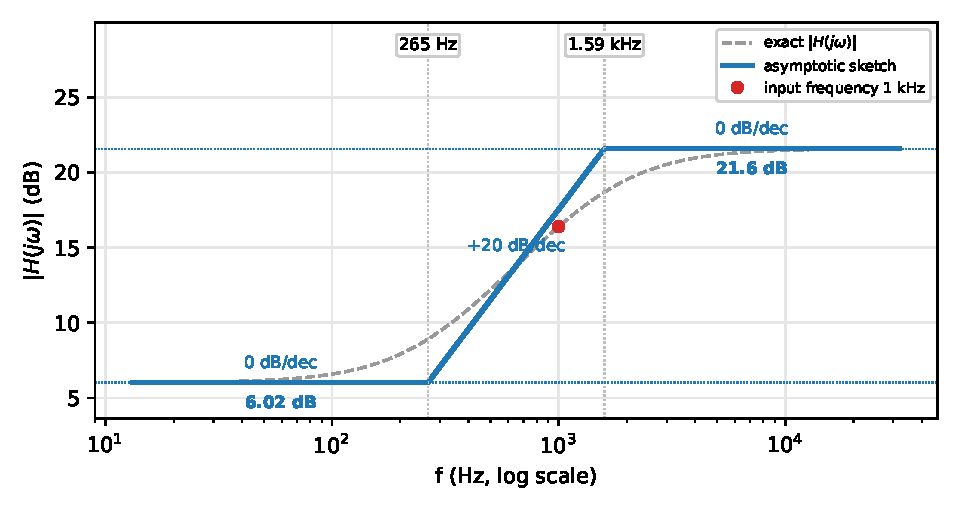
\includegraphics[width=0.78\linewidth,height=6.5cm,keepaspectratio]{p09_bode}\end{center}

{\small Blue: the straight-line sketch you are expected to draw. Dashed grey: the exact curve (about 3\,dB below the corner of an isolated pole). Red dot: the input frequency of Step 7.}
\solstep{7}{Steady-state output}The input is $V_i(t) = 0.1\sin\left(2\pi\cdot 1000\,t\right)$, so $\omega_{in} = 2\pi\cdot 1000 = 6280$\,rad/s. Put $s=j\omega_{in}$ in each factor (tool T5): magnitudes multiply, angles add.
{\small Rules: $\left|\frac{s}{s+p}\right| = \frac{\omega}{\sqrt{\omega^2+p^2}}$, $\angle = \frac{\pi}{2}-\tan^{-1}\frac{\omega}{p}$;\quad $\left|\frac{1}{1+s/p}\right| = \frac{1}{\sqrt{1+(\omega/p)^2}}$, $\angle = -\tan^{-1}\frac{\omega}{p}$;\quad $\left|1+\frac{s}{z}\right| = \sqrt{1+(\omega/z)^2}$, $\angle = \tan^{-1}\frac{\omega}{z}$;\quad a negative $K$ adds $-\pi$.}
\begin{center}\renewcommand{\arraystretch}{1.35}
\begin{tabular}{ccc}
\toprule
factor & magnitude & angle (rad) \\
\midrule
$-2$ & $2$ & $-3.14$ \\
$\rule[-1.1em]{0pt}{2.8em}\left(1+\dfrac{s}{2\pi\cdot 265}\right)$ & $3.9$ & $1.31$ \\
$\rule[-1.7em]{0pt}{4em}\dfrac{1}{1+\dfrac{s}{2\pi\cdot 1.59\mathrm{k}}}$ & $0.8467$ & $-0.561$ \\
\textbf{total} & $\mathbf{6.605}$ (product) & $\mathbf{-2.39}$ (sum) \\
\bottomrule
\end{tabular}\end{center}

\begin{align*}
|H(j\omega_{in})| &= 6.61, \qquad \angle H(j\omega_{in}) = -2.39\ \mathrm{rad} \\
v_{o,ac}(t) &= 6.61\times 0.1\,\sin\left(2\pi\cdot 1000\,t - 2.39\right) = 0.661\,\sin\left(2\pi\cdot 1000\,t - 2.39\right)
\end{align*}

\[
\boxed{V_o(t) = 0.661\,\sin\left(2\pi\cdot 1000\,t - 2.39\right)\ \mathrm{V}}
\]

\begin{ansbox}
$H(s) = -2\,\left(1+\dfrac{s}{2\pi\cdot 265}\right)\,\dfrac{1}{1+\dfrac{s}{2\pi\cdot 1.59\mathrm{k}}}$\quad (corners: 265 Hz, 1.59 kHz)\\[4pt]
$V_o(t) = 0.661\,\sin\left(2\pi\cdot 1000\,t - 2.39\right)\ \mathrm{V}$
\end{ansbox}

\newpage
\subsection*{Solution 2A.10 \hfill Medium}
\begin{center}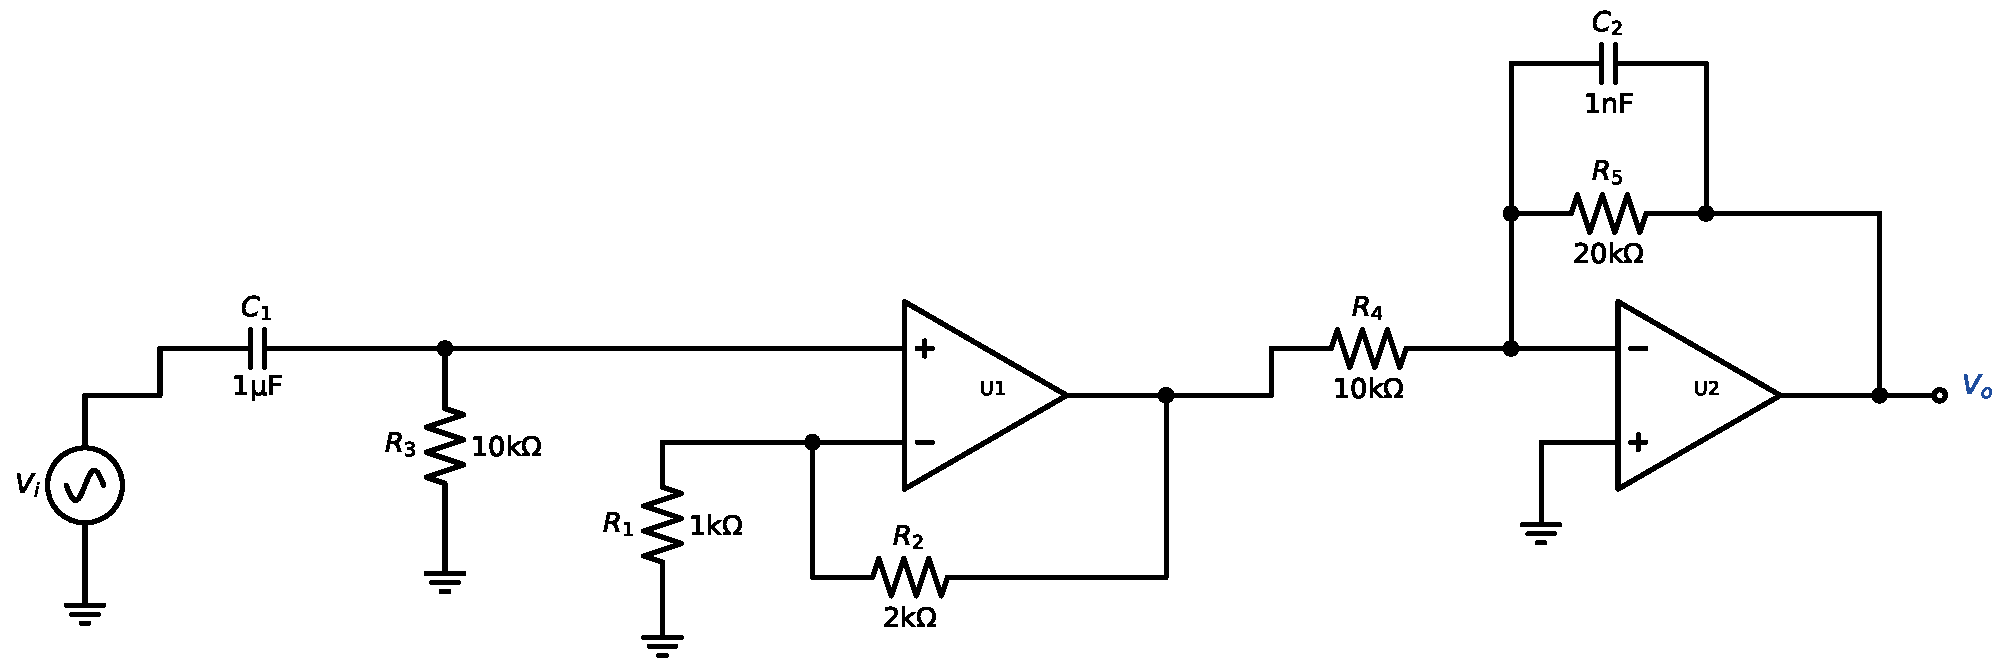
\includegraphics[width=\linewidth,height=5cm,keepaspectratio]{p10_circuit}\end{center}
\solstep{1}{Identify the sources}Independent sources: the AC input $V_i(t)$. No DC source: $V_{o,dc}=0$ and Step 2 is skipped.
\solstep{2}{DC circuit}No DC sources: $V_{o,dc}=0$.
\solstep{3}{Op-amp rules}Each op-amp has negative feedback (its output is connected back to its $-$ input), so with an ideal op-amp (tool T1): (a) no current flows into the $+$ or $-$ input; (b) $V_-=V_+$ (virtual short). The circuit is a cascade of standard blocks, so each block is solved with its block formula (tool T2).
\solstep{4}{Transfer function, block by block}Each op-amp output is an ideal voltage source, so a block's output does not change when the next block is connected: the blocks can be solved one at a time and multiplied.\[
H(s) = \frac{V_o}{V_i} = \frac{V_{o1}}{V_{i}}\cdot\frac{V_{o}}{V_{o1}}
\]

\textbf{Block 1 (U1).} Non-inverting block: No current flows into the $+$ input, so $R_{3}$ and $\frac{1}{sC_{1}}$ form a plain voltage divider: $V_+ = \frac{R_{3}}{\frac{1}{sC_{1}} + R_{3}}V_{i}$. The op-amp forces $V_-=V_+$, and $R_{1}$, $R_{2}$ divide the output: $V_- = \frac{R_{1}}{R_{1} + R_{2}}V_{o1}$, hence $V_{o1} = \left(1+\frac{R_{2}}{R_{1}}\right)V_+$.\[
\frac{V_{o1}}{V_{i}} = \frac{R_{3}}{\frac{1}{sC_{1}} + R_{3}}\left(1+\frac{R_{2}}{R_{1}}\right) = \dfrac{3\,s}{s + 100}
\]

\textbf{Block 2 (U2).} Inverting block: the $+$ input is grounded, so $V_- = V_+ = 0$ (virtual ground). The current $\frac{V_{o1} - 0}{R_{4}}$ through $R_{4}$ cannot enter the op-amp, so all of it flows through $Z_{f2}$: $V_{o} = 0 - Z_{f2}\cdot\frac{V_{o1}}{R_{4}}$.\begin{align*}
Z_{f2} &= R_{5} \parallel \frac{1}{sC_{2}} = \dfrac{10^{9}}{s + 50000}
\end{align*}
\[
\frac{V_{o}}{V_{o1}} = -\frac{Z_{f2}}{R_{4}} = \dfrac{-10^{5}}{s + 50000}
\]

Multiply the blocks and simplify:\[
H(s) = \dfrac{-3\times 10^{5}\,s}{s^{2} + 50100\,s + 5\times 10^{6}}
\]

\solstep{5}{Standard (Bode-ready) form}Find the roots. Every root $s=-p$ of the denominator is a \emph{pole}, every root $s=-z$ of the numerator is a \emph{zero}; $|p|$ and $|z|$ are the corner frequencies (rad/s).
\begin{itemize}[leftmargin=*,itemsep=2pt]
\item Numerator: it has the factor $s$ $\Rightarrow$ 1 zero at $s=0$.
\item Denominator: $s^{2} + 50100\,s + 5\times 10^{6}$; quadratic formula:\[
s = \frac{-50100 \pm \sqrt{(50100)^2 - 4(5\times 10^{6})}}{2} = \frac{-50100 \pm 49900}{2} \Rightarrow s = -100,\ -50000
\]

\end{itemize}

Factored form (leading coefficient in front):
\[
H(s) = -3\times 10^{5}\,\dfrac{s}{(s+100)(s+50000)}
\]

Bode-ready form: rewrite every $(s+p) = p\left(1+\frac{s}{p}\right)$ and $(s+z) = z\left(1+\frac{s}{z}\right)$, and collect all constants into $K$. Each $s$ in the numerator is paired with one of the \emph{lowest} poles as $\frac{s}{s+p}$ (that factor is $\approx 1$ above $p$). Then every factor except $K$ is $\approx 1$ inside the pass-band:
\[
H(s) = -6\,\dfrac{s}{s+2\pi\cdot 15.9}\,\dfrac{1}{1+\dfrac{s}{2\pi\cdot 7.96\mathrm{k}}},\qquad K = -6
\]

\begin{center}\renewcommand{\arraystretch}{1.35}
\begin{tabular}{cccc}
\toprule
type & $\omega_c$ (rad/s) & $f_c=\omega_c/2\pi$ & slope change \\
\midrule
pole & $100$ & 15.9 Hz & $-20$ dB/dec \\
pole & $50000$ & 7.96 kHz & $-20$ dB/dec \\
\bottomrule
\end{tabular}\end{center}

\solstep{6}{Magnitude Bode plot}Below every corner $|H(s)|\approx 0.06\,s$, so the plot starts with a slope of $+20$\,dB/dec. Then, moving right, each pole bends the line down by 20\,dB/dec and each zero bends it up by 20\,dB/dec (tool T6):
\begin{center}\renewcommand{\arraystretch}{1.35}
\begin{tabular}{lcl}
\toprule
frequency range & slope & asymptote level \\
\midrule
$f<$ 15.9 Hz & $+20$ dB/dec & 15.6 dB at end \\
15.9 Hz -- 7.96 kHz & $0$ dB/dec (flat) & 15.6 dB at start, 15.6 dB at end \\
$f>$ 7.96 kHz & $-20$ dB/dec & 15.6 dB at start \\
\bottomrule
\end{tabular}\end{center}

The flat (pass-band) level is $20\log_{10}|K| = 20\log_{10}6 = 15.6$\,dB.
\begin{center}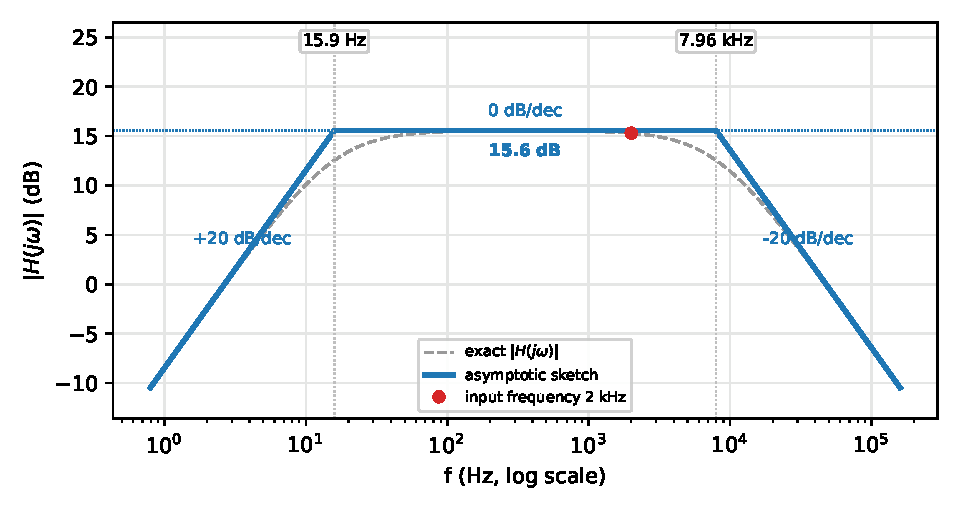
\includegraphics[width=0.78\linewidth,height=6.5cm,keepaspectratio]{p10_bode}\end{center}

{\small Blue: the straight-line sketch you are expected to draw. Dashed grey: the exact curve (about 3\,dB below the corner of an isolated pole). Red dot: the input frequency of Step 7.}
\solstep{7}{Steady-state output}The input is $V_i(t) = 0.1\sin\left(2\pi\cdot 2000\,t\right)$, so $\omega_{in} = 2\pi\cdot 2000 = 12600$\,rad/s. Put $s=j\omega_{in}$ in each factor (tool T5): magnitudes multiply, angles add.
{\small Rules: $\left|\frac{s}{s+p}\right| = \frac{\omega}{\sqrt{\omega^2+p^2}}$, $\angle = \frac{\pi}{2}-\tan^{-1}\frac{\omega}{p}$;\quad $\left|\frac{1}{1+s/p}\right| = \frac{1}{\sqrt{1+(\omega/p)^2}}$, $\angle = -\tan^{-1}\frac{\omega}{p}$;\quad $\left|1+\frac{s}{z}\right| = \sqrt{1+(\omega/z)^2}$, $\angle = \tan^{-1}\frac{\omega}{z}$;\quad a negative $K$ adds $-\pi$.}
\begin{center}\renewcommand{\arraystretch}{1.35}
\begin{tabular}{ccc}
\toprule
factor & magnitude & angle (rad) \\
\midrule
$-6$ & $6$ & $-3.14$ \\
$\rule[-1.1em]{0pt}{2.8em}\dfrac{s}{s+2\pi\cdot 15.9}$ & $1$ & $0.00796$ \\
$\rule[-1.7em]{0pt}{4em}\dfrac{1}{1+\dfrac{s}{2\pi\cdot 7.96\mathrm{k}}}$ & $0.9698$ & $-0.246$ \\
\textbf{total} & $\mathbf{5.819}$ (product) & $\mathbf{-3.38}$ (sum) \\
\bottomrule
\end{tabular}\end{center}

\begin{align*}
|H(j\omega_{in})| &= 5.82, \qquad \angle H(j\omega_{in}) = -3.38\ \mathrm{rad} \\
v_{o,ac}(t) &= 5.82\times 0.1\,\sin\left(2\pi\cdot 2000\,t - 3.38\right) = 0.582\,\sin\left(2\pi\cdot 2000\,t - 3.38\right)
\end{align*}

\[
\boxed{V_o(t) = 0.582\,\sin\left(2\pi\cdot 2000\,t - 3.38\right)\ \mathrm{V}}
\]

\begin{ansbox}
$H(s) = -6\,\dfrac{s}{s+2\pi\cdot 15.9}\,\dfrac{1}{1+\dfrac{s}{2\pi\cdot 7.96\mathrm{k}}}$\quad (corners: 15.9 Hz, 7.96 kHz)\\[4pt]
$V_o(t) = 0.582\,\sin\left(2\pi\cdot 2000\,t - 3.38\right)\ \mathrm{V}$
\end{ansbox}

\newpage
\subsection*{Solution 2A.11 \hfill Medium}
\begin{center}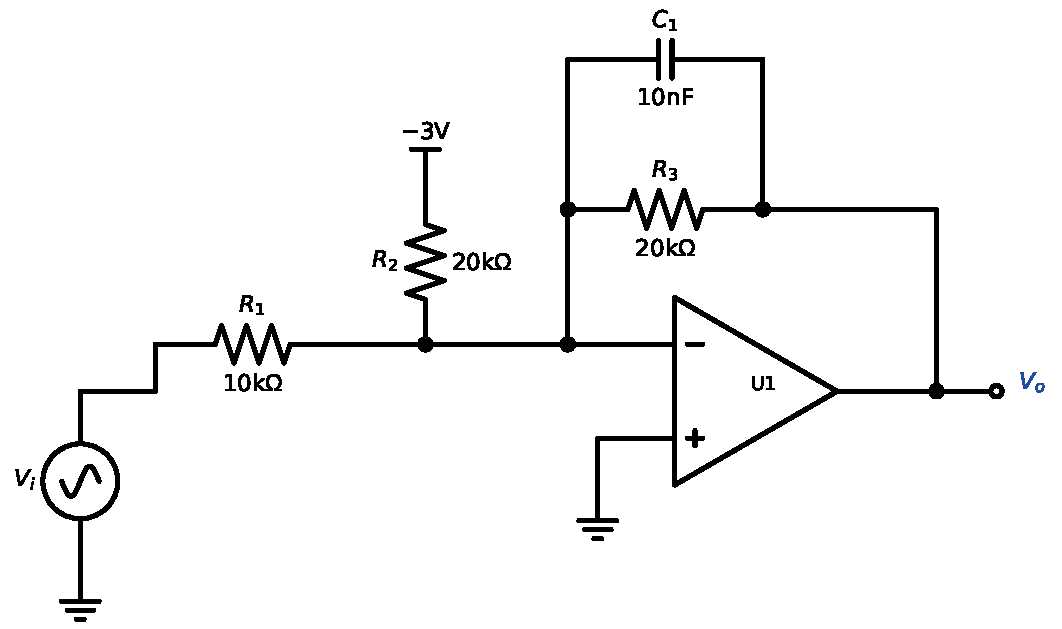
\includegraphics[width=\linewidth,height=5cm,keepaspectratio]{p11_circuit}\end{center}
\solstep{1}{Identify the sources}Independent sources: the AC input $V_i(t)$ and the DC supply $-3\,\mathrm{V}$. Both DC and AC are present, so use superposition: $V_o(t) = V_{o,dc}+v_{o,ac}(t)$. The DC part is Step 2, the AC part Steps 3--7.
\solstep{2}{DC circuit $\Rightarrow V_{o,dc}$}DC rules: $V_i=0$ and every capacitor is an open circuit (no inductors appear in these circuits). A block passes DC with its gain at $s=0$, i.e. $H_k(0)$.
\begin{enumerate}[leftmargin=*,itemsep=2pt]
\item Block 1 (summer): its input has no DC. Only the supply drives a DC current, $\frac{V_{DC}}{R_{2}}$, through $Z_{f1}$ (at DC $R_{2}=20\,\mathrm{k}\Omega$, $Z_{f1}=20\,\mathrm{k}\Omega$):\[
V_{o}\big|_{dc} = -Z_{f1}\frac{V_{DC}}{R_{2}} = -20\,\mathrm{k}\cdot\frac{-3}{20\,\mathrm{k}} = 3\,\mathrm{V}
\]

\end{enumerate}

\[
\boxed{V_{o,dc} = 3\,\mathrm{V}}
\]

\solstep{3}{Op-amp rules}The op-amp has negative feedback (its output is connected back to its $-$ input), so with an ideal op-amp (tool T1): (a) no current flows into the $+$ or $-$ input; (b) $V_-=V_+$ (virtual short). The circuit is a standard block, so use its block formula (tool T2).
\solstep{4}{Transfer function, block by block}\textbf{Block 1 (U1).} Summing block: $V_-=V_+=0$ (virtual ground), so the input currents $\frac{V_{i}}{R_{1}}$ and $\frac{V_{DC}}{R_{2}}$ simply add and both flow through $Z_{f1}$: $V_{o} = -Z_{f1}\left(\frac{V_{i}}{R_{1}} + \frac{V_{DC}}{R_{2}}\right)$. For the AC part the supply is zero, so $R_{2}$ (from virtual ground to AC ground) carries no AC current and drops out.\begin{align*}
Z_{f1} &= R_{3} \parallel \frac{1}{sC_{1}} = \dfrac{10^{8}}{s + 5000}
\end{align*}
\[
\frac{V_{o}}{V_{i}} = -\frac{Z_{f1}}{R_{1}} = \dfrac{-10000}{s + 5000}
\]

So:\[
H(s) = \dfrac{-10000}{s + 5000}
\]

\solstep{5}{Standard (Bode-ready) form}Find the roots. Every root $s=-p$ of the denominator is a \emph{pole}, every root $s=-z$ of the numerator is a \emph{zero}; $|p|$ and $|z|$ are the corner frequencies (rad/s).
\begin{itemize}[leftmargin=*,itemsep=2pt]
\item Denominator: $s + 5000$; $s + 5000 = 0 \Rightarrow s = -5000$.
\end{itemize}

Factored form (leading coefficient in front):
\[
H(s) = -10000\,\dfrac{1}{(s+5000)}
\]

Bode-ready form: rewrite every $(s+p) = p\left(1+\frac{s}{p}\right)$ and $(s+z) = z\left(1+\frac{s}{z}\right)$, and collect all constants into $K$. Then every factor except $K$ is $\approx 1$ inside the pass-band:
\[
H(s) = -2\,\dfrac{1}{1+\dfrac{s}{2\pi\cdot 796}},\qquad K = -2
\]

\begin{center}\renewcommand{\arraystretch}{1.35}
\begin{tabular}{cccc}
\toprule
type & $\omega_c$ (rad/s) & $f_c=\omega_c/2\pi$ & slope change \\
\midrule
pole & $5000$ & 796 Hz & $-20$ dB/dec \\
\bottomrule
\end{tabular}\end{center}

\solstep{6}{Magnitude Bode plot}Below every corner, all factors are $\approx$ constant: $|H| \approx 2$ $= 6.02$\,dB (flat, 0 dB/dec). Then, moving right, each pole bends the line down by 20\,dB/dec and each zero bends it up by 20\,dB/dec (tool T6):
\begin{center}\renewcommand{\arraystretch}{1.35}
\begin{tabular}{lcl}
\toprule
frequency range & slope & asymptote level \\
\midrule
$f<$ 796 Hz & $0$ dB/dec (flat) & 6.02 dB at end \\
$f>$ 796 Hz & $-20$ dB/dec & 6.02 dB at start \\
\bottomrule
\end{tabular}\end{center}

The flat (pass-band) level is $20\log_{10}|K| = 20\log_{10}2 = 6.02$\,dB.
\begin{center}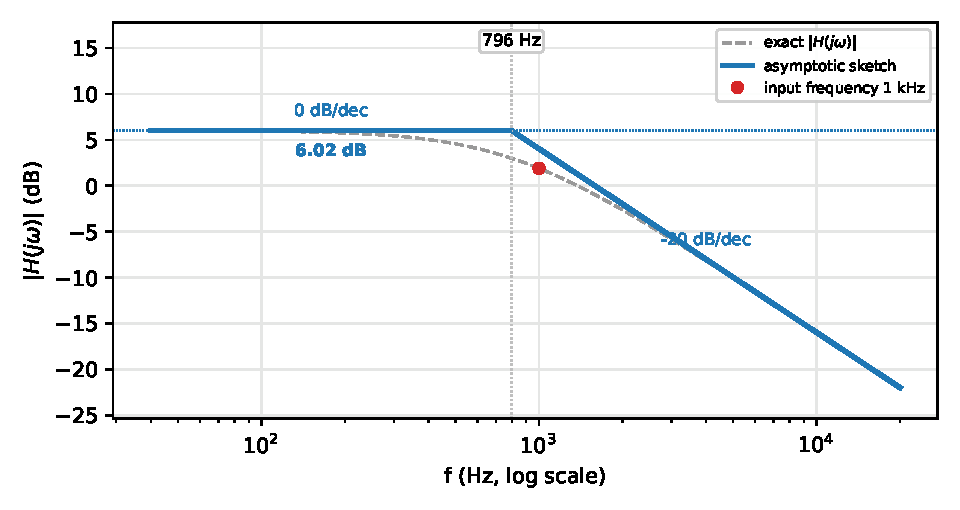
\includegraphics[width=0.78\linewidth,height=6.5cm,keepaspectratio]{p11_bode}\end{center}

{\small Blue: the straight-line sketch you are expected to draw. Dashed grey: the exact curve (about 3\,dB below the corner of an isolated pole). Red dot: the input frequency of Step 7.}
\solstep{7}{Steady-state output}The input is $V_i(t) = 0.5\sin\left(2\pi\cdot 1000\,t\right)$, so $\omega_{in} = 2\pi\cdot 1000 = 6280$\,rad/s. Put $s=j\omega_{in}$ in each factor (tool T5): magnitudes multiply, angles add.
{\small Rules: $\left|\frac{s}{s+p}\right| = \frac{\omega}{\sqrt{\omega^2+p^2}}$, $\angle = \frac{\pi}{2}-\tan^{-1}\frac{\omega}{p}$;\quad $\left|\frac{1}{1+s/p}\right| = \frac{1}{\sqrt{1+(\omega/p)^2}}$, $\angle = -\tan^{-1}\frac{\omega}{p}$;\quad $\left|1+\frac{s}{z}\right| = \sqrt{1+(\omega/z)^2}$, $\angle = \tan^{-1}\frac{\omega}{z}$;\quad a negative $K$ adds $-\pi$.}
\begin{center}\renewcommand{\arraystretch}{1.35}
\begin{tabular}{ccc}
\toprule
factor & magnitude & angle (rad) \\
\midrule
$-2$ & $2$ & $-3.14$ \\
$\rule[-1.7em]{0pt}{4em}\dfrac{1}{1+\dfrac{s}{2\pi\cdot 796}}$ & $0.6227$ & $-0.899$ \\
\textbf{total} & $\mathbf{1.245}$ (product) & $\mathbf{-4.04}$ (sum) \\
\bottomrule
\end{tabular}\end{center}

\begin{align*}
|H(j\omega_{in})| &= 1.25, \qquad \angle H(j\omega_{in}) = -4.04\ \mathrm{rad} \\
v_{o,ac}(t) &= 1.25\times 0.5\,\sin\left(2\pi\cdot 1000\,t - 4.04\right) = 0.623\,\sin\left(2\pi\cdot 1000\,t - 4.04\right)
\end{align*}

Add the DC part from Step 2 (superposition):
\[
\boxed{V_o(t) = 3 + 0.623\,\sin\left(2\pi\cdot 1000\,t - 4.04\right)\ \mathrm{V}}
\]

\begin{ansbox}
$H(s) = -2\,\dfrac{1}{1+\dfrac{s}{2\pi\cdot 796}}$\quad (corners: 796 Hz)\\[4pt]
$V_o(t) = 3 + 0.623\,\sin\left(2\pi\cdot 1000\,t - 4.04\right)\ \mathrm{V}$
\end{ansbox}

\newpage
\subsection*{Solution 2A.12 \hfill Medium}
\begin{center}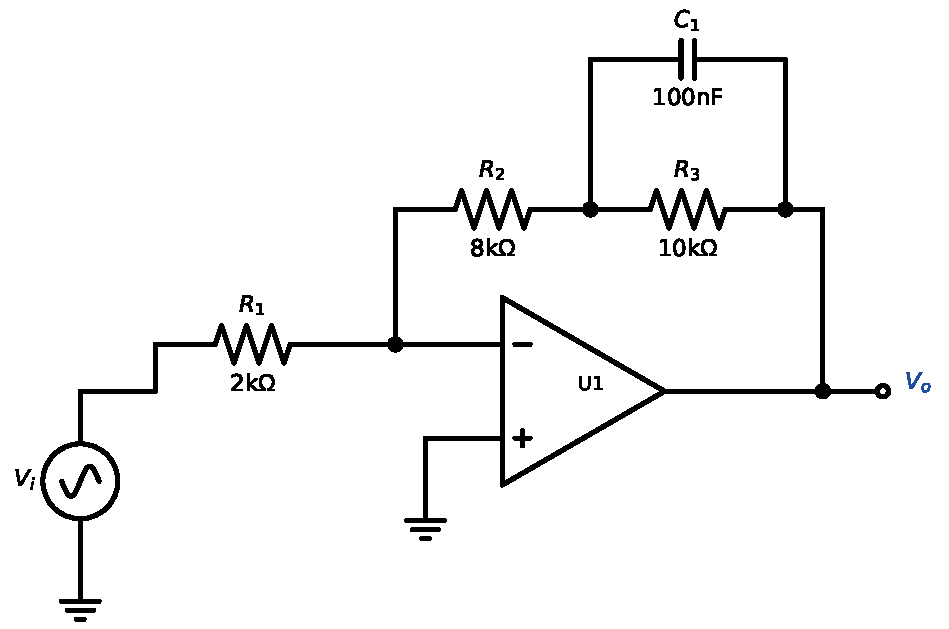
\includegraphics[width=\linewidth,height=5cm,keepaspectratio]{p12_circuit}\end{center}
\solstep{1}{Identify the sources}Independent sources: the AC input $V_i(t)$. No DC source: $V_{o,dc}=0$ and Step 2 is skipped.
\solstep{2}{DC circuit}No DC sources: $V_{o,dc}=0$.
\solstep{3}{Op-amp rules}The op-amp has negative feedback (its output is connected back to its $-$ input), so with an ideal op-amp (tool T1): (a) no current flows into the $+$ or $-$ input; (b) $V_-=V_+$ (virtual short). The circuit is a standard block, so use its block formula (tool T2).
\solstep{4}{Transfer function, block by block}\textbf{Block 1 (U1).} Inverting block: the $+$ input is grounded, so $V_- = V_+ = 0$ (virtual ground). The current $\frac{V_{i} - 0}{R_{1}}$ through $R_{1}$ cannot enter the op-amp, so all of it flows through $Z_{f1}$: $V_{o} = 0 - Z_{f1}\cdot\frac{V_{i}}{R_{1}}$.\begin{align*}
Z_{f1} &= R_{2} + \left(R_{3} \parallel \frac{1}{sC_{1}}\right) = \dfrac{8000\,s + 1.8\times 10^{7}}{s + 1000}
\end{align*}
\[
\frac{V_{o}}{V_{i}} = -\frac{Z_{f1}}{R_{1}} = \dfrac{-4\,s - 9000}{s + 1000}
\]

So:\[
H(s) = \dfrac{-4\,s - 9000}{s + 1000}
\]

\solstep{5}{Standard (Bode-ready) form}Find the roots. Every root $s=-p$ of the denominator is a \emph{pole}, every root $s=-z$ of the numerator is a \emph{zero}; $|p|$ and $|z|$ are the corner frequencies (rad/s).
\begin{itemize}[leftmargin=*,itemsep=2pt]
\item Numerator: $-4\,s - 9000$; divide by the leading coefficient $-4$ (this does not move the roots): $s + 2250$; $s + 2250 = 0 \Rightarrow s = -2250$.
\item Denominator: $s + 1000$; $s + 1000 = 0 \Rightarrow s = -1000$.
\end{itemize}

Factored form (leading coefficient in front):
\[
H(s) = -4\,\dfrac{(s+2250)}{(s+1000)}
\]

Bode-ready form: rewrite every $(s+p) = p\left(1+\frac{s}{p}\right)$ and $(s+z) = z\left(1+\frac{s}{z}\right)$, and collect all constants into $K$. Then every factor except $K$ is $\approx 1$ inside the pass-band:
\[
H(s) = -9\,\dfrac{1}{1+\dfrac{s}{2\pi\cdot 159}}\,\left(1+\dfrac{s}{2\pi\cdot 358}\right),\qquad K = -9
\]

\begin{center}\renewcommand{\arraystretch}{1.35}
\begin{tabular}{cccc}
\toprule
type & $\omega_c$ (rad/s) & $f_c=\omega_c/2\pi$ & slope change \\
\midrule
pole & $1000$ & 159 Hz & $-20$ dB/dec \\
zero & $2250$ & 358 Hz & $+20$ dB/dec \\
\bottomrule
\end{tabular}\end{center}

\solstep{6}{Magnitude Bode plot}Below every corner, all factors are $\approx$ constant: $|H| \approx 9$ $= 19.1$\,dB (flat, 0 dB/dec). Then, moving right, each pole bends the line down by 20\,dB/dec and each zero bends it up by 20\,dB/dec (tool T6):
\begin{center}\renewcommand{\arraystretch}{1.35}
\begin{tabular}{lcl}
\toprule
frequency range & slope & asymptote level \\
\midrule
$f<$ 159 Hz & $0$ dB/dec (flat) & 19.1 dB at end \\
159 Hz -- 358 Hz & $-20$ dB/dec & 19.1 dB at start, 12 dB at end \\
$f>$ 358 Hz & $0$ dB/dec (flat) & 12 dB at start \\
\bottomrule
\end{tabular}\end{center}

\begin{center}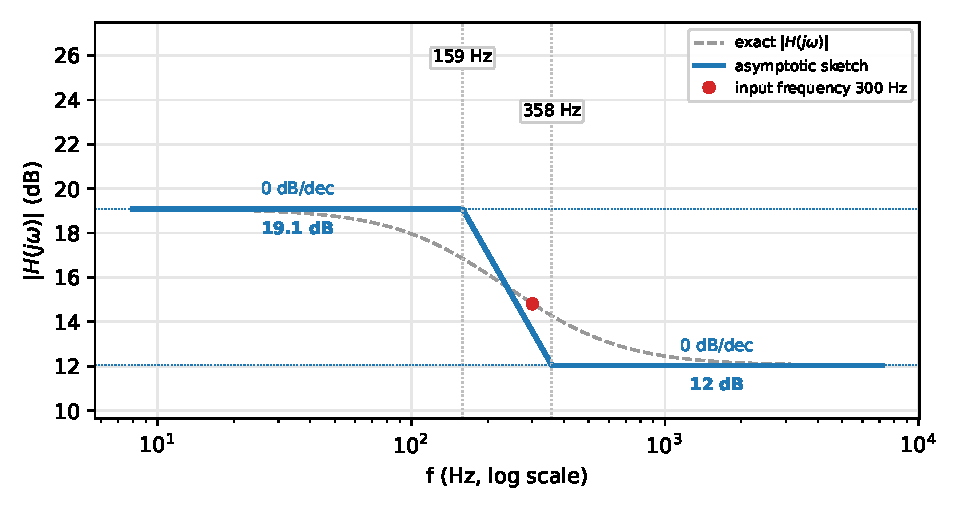
\includegraphics[width=0.78\linewidth,height=6.5cm,keepaspectratio]{p12_bode}\end{center}

{\small Blue: the straight-line sketch you are expected to draw. Dashed grey: the exact curve (about 3\,dB below the corner of an isolated pole). Red dot: the input frequency of Step 7.}
\solstep{7}{Steady-state output}The input is $V_i(t) = 0.2\sin\left(2\pi\cdot 300\,t\right)$, so $\omega_{in} = 2\pi\cdot 300 = 1880$\,rad/s. Put $s=j\omega_{in}$ in each factor (tool T5): magnitudes multiply, angles add.
{\small Rules: $\left|\frac{s}{s+p}\right| = \frac{\omega}{\sqrt{\omega^2+p^2}}$, $\angle = \frac{\pi}{2}-\tan^{-1}\frac{\omega}{p}$;\quad $\left|\frac{1}{1+s/p}\right| = \frac{1}{\sqrt{1+(\omega/p)^2}}$, $\angle = -\tan^{-1}\frac{\omega}{p}$;\quad $\left|1+\frac{s}{z}\right| = \sqrt{1+(\omega/z)^2}$, $\angle = \tan^{-1}\frac{\omega}{z}$;\quad a negative $K$ adds $-\pi$.}
\begin{center}\renewcommand{\arraystretch}{1.35}
\begin{tabular}{ccc}
\toprule
factor & magnitude & angle (rad) \\
\midrule
$-9$ & $9$ & $-3.14$ \\
$\rule[-1.7em]{0pt}{4em}\dfrac{1}{1+\dfrac{s}{2\pi\cdot 159}}$ & $0.4686$ & $-1.08$ \\
$\rule[-1.1em]{0pt}{2.8em}\left(1+\dfrac{s}{2\pi\cdot 358}\right)$ & $1.305$ & $0.697$ \\
\textbf{total} & $\mathbf{5.502}$ (product) & $\mathbf{-3.53}$ (sum) \\
\bottomrule
\end{tabular}\end{center}

\begin{align*}
|H(j\omega_{in})| &= 5.5, \qquad \angle H(j\omega_{in}) = -3.53\ \mathrm{rad} \\
v_{o,ac}(t) &= 5.5\times 0.2\,\sin\left(2\pi\cdot 300\,t - 3.53\right) = 1.1\,\sin\left(2\pi\cdot 300\,t - 3.53\right)
\end{align*}

\[
\boxed{V_o(t) = 1.1\,\sin\left(2\pi\cdot 300\,t - 3.53\right)\ \mathrm{V}}
\]

\begin{ansbox}
$H(s) = -9\,\dfrac{1}{1+\dfrac{s}{2\pi\cdot 159}}\,\left(1+\dfrac{s}{2\pi\cdot 358}\right)$\quad (corners: 159 Hz, 358 Hz)\\[4pt]
$V_o(t) = 1.1\,\sin\left(2\pi\cdot 300\,t - 3.53\right)\ \mathrm{V}$
\end{ansbox}

\newpage
\subsection*{Solution 2A.13 \hfill Hard}
\begin{center}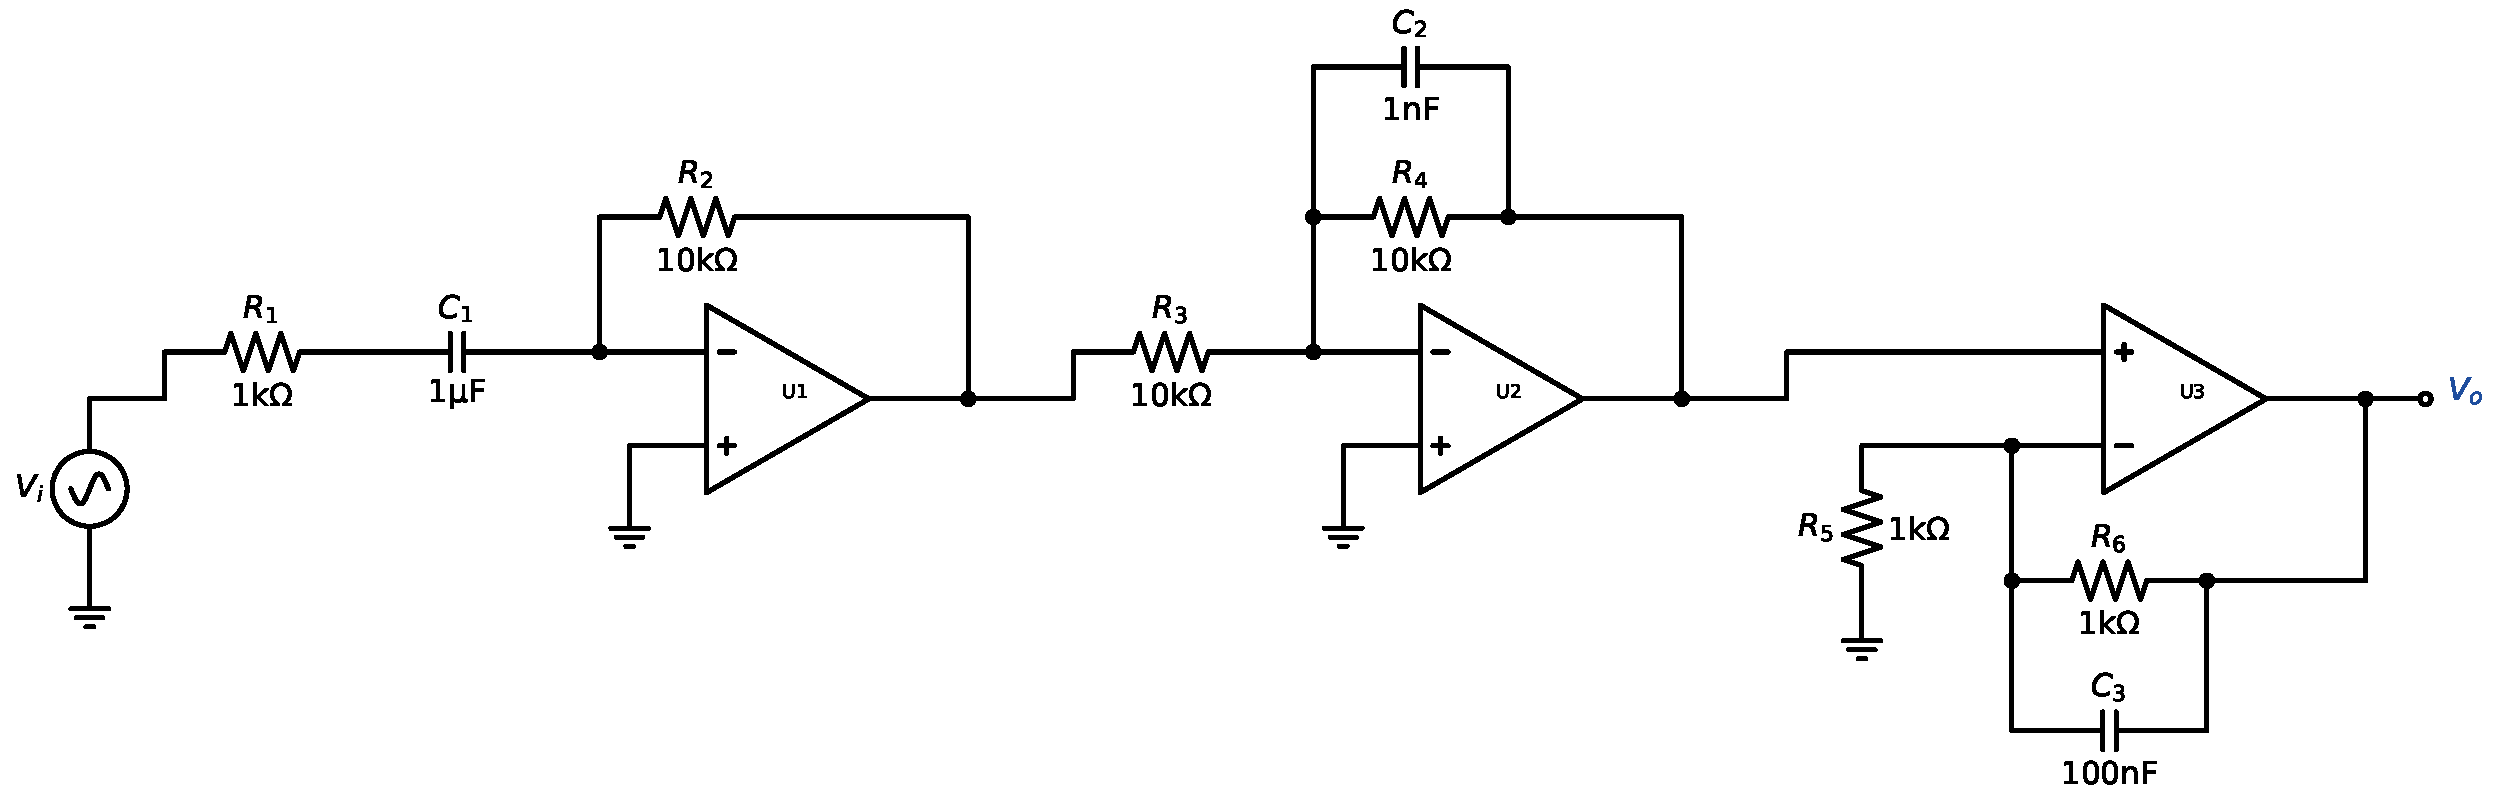
\includegraphics[width=\linewidth,height=5cm,keepaspectratio]{p13_circuit}\end{center}
\solstep{1}{Identify the sources}Independent sources: the AC input $V_i(t)$. No DC source: $V_{o,dc}=0$ and Step 2 is skipped.
\solstep{2}{DC circuit}No DC sources: $V_{o,dc}=0$.
\solstep{3}{Op-amp rules}Each op-amp has negative feedback (its output is connected back to its $-$ input), so with an ideal op-amp (tool T1): (a) no current flows into the $+$ or $-$ input; (b) $V_-=V_+$ (virtual short). The circuit is a cascade of standard blocks, so each block is solved with its block formula (tool T2).
\solstep{4}{Transfer function, block by block}Each op-amp output is an ideal voltage source, so a block's output does not change when the next block is connected: the blocks can be solved one at a time and multiplied.\[
H(s) = \frac{V_o}{V_i} = \frac{V_{o1}}{V_{i}}\cdot\frac{V_{o2}}{V_{o1}}\cdot\frac{V_{o}}{V_{o2}}
\]

\textbf{Block 1 (U1).} Inverting block: the $+$ input is grounded, so $V_- = V_+ = 0$ (virtual ground). The current $\frac{V_{i} - 0}{Z_{in1}}$ through $Z_{in1}$ cannot enter the op-amp, so all of it flows through $R_{2}$: $V_{o1} = 0 - R_{2}\cdot\frac{V_{i}}{Z_{in1}}$.\begin{align*}
Z_{in1} &= R_{1} + \frac{1}{sC_{1}} = \dfrac{1000\,s + 10^{6}}{s}
\end{align*}
\[
\frac{V_{o1}}{V_{i}} = -\frac{R_{2}}{Z_{in1}} = \dfrac{-10\,s}{s + 1000}
\]

\textbf{Block 2 (U2).} Inverting block: the $+$ input is grounded, so $V_- = V_+ = 0$ (virtual ground). The current $\frac{V_{o1} - 0}{R_{3}}$ through $R_{3}$ cannot enter the op-amp, so all of it flows through $Z_{f2}$: $V_{o2} = 0 - Z_{f2}\cdot\frac{V_{o1}}{R_{3}}$.\begin{align*}
Z_{f2} &= R_{4} \parallel \frac{1}{sC_{2}} = \dfrac{10^{9}}{s + 10^{5}}
\end{align*}
\[
\frac{V_{o2}}{V_{o1}} = -\frac{Z_{f2}}{R_{3}} = \dfrac{-10^{5}}{s + 10^{5}}
\]

\textbf{Block 3 (U3).} Non-inverting block: The $+$ input is the block input: $V_+ = V_{o2}$. The op-amp forces $V_-=V_+$, and $R_{5}$, $Z_{f3}$ divide the output: $V_- = \frac{R_{5}}{R_{5} + Z_{f3}}V_{o}$, hence $V_{o} = \left(1+\frac{Z_{f3}}{R_{5}}\right)V_+$.\begin{align*}
Z_{f3} &= R_{6} \parallel \frac{1}{sC_{3}} = \dfrac{10^{7}}{s + 10000}
\end{align*}
\[
\frac{V_{o}}{V_{o2}} = \left(1+\frac{Z_{f3}}{R_{5}}\right) = \dfrac{s + 20000}{s + 10000}
\]

Multiply the blocks and simplify:\[
H(s) = \dfrac{10^{6}\,s^{2} + 2\times 10^{10}\,s}{s^{3} + 1.11\times 10^{5}\,s^{2} + 1.11\times 10^{9}\,s + 10^{12}}
\]

\solstep{5}{Standard (Bode-ready) form}Find the roots. Every root $s=-p$ of the denominator is a \emph{pole}, every root $s=-z$ of the numerator is a \emph{zero}; $|p|$ and $|z|$ are the corner frequencies (rad/s).
\begin{itemize}[leftmargin=*,itemsep=2pt]
\item Numerator: it has the factor $s$ $\Rightarrow$ 1 zero at $s=0$.
\item Numerator (after taking out the $s$ factor): $10^{6}\,s + 2\times 10^{10}$; divide by the leading coefficient $10^{6}$ (this does not move the roots): $s + 20000$; $s + 20000 = 0 \Rightarrow s = -20000$.
\item Denominator: $s^{3} + 1.11\times 10^{5}\,s^{2} + 1.11\times 10^{9}\,s + 10^{12}$; this is degree 3: use a calculator's polynomial solver (or \texttt{numpy.roots}) $\Rightarrow s = -1000,\ -10000,\ -100000$.
\end{itemize}

Factored form (leading coefficient in front):
\[
H(s) = 10^{6}\,\dfrac{s(s+20000)}{(s+1000)(s+10000)(s+10^{5})}
\]

Bode-ready form: rewrite every $(s+p) = p\left(1+\frac{s}{p}\right)$ and $(s+z) = z\left(1+\frac{s}{z}\right)$, and collect all constants into $K$. Each $s$ in the numerator is paired with one of the \emph{lowest} poles as $\frac{s}{s+p}$ (that factor is $\approx 1$ above $p$). Then every factor except $K$ is $\approx 1$ inside the pass-band:
\[
H(s) = 20\,\dfrac{s}{s+2\pi\cdot 159}\,\dfrac{1}{1+\dfrac{s}{2\pi\cdot 1.59\mathrm{k}}}\,\left(1+\dfrac{s}{2\pi\cdot 3.18\mathrm{k}}\right)\,\dfrac{1}{1+\dfrac{s}{2\pi\cdot 15.9\mathrm{k}}},\qquad K = 20
\]

\begin{center}\renewcommand{\arraystretch}{1.35}
\begin{tabular}{cccc}
\toprule
type & $\omega_c$ (rad/s) & $f_c=\omega_c/2\pi$ & slope change \\
\midrule
pole & $1000$ & 159 Hz & $-20$ dB/dec \\
pole & $10000$ & 1.59 kHz & $-20$ dB/dec \\
zero & $20000$ & 3.18 kHz & $+20$ dB/dec \\
pole & $10^{5}$ & 15.9 kHz & $-20$ dB/dec \\
\bottomrule
\end{tabular}\end{center}

\solstep{6}{Magnitude Bode plot}Below every corner $|H(s)|\approx 0.02\,s$, so the plot starts with a slope of $+20$\,dB/dec. Then, moving right, each pole bends the line down by 20\,dB/dec and each zero bends it up by 20\,dB/dec (tool T6):
\begin{center}\renewcommand{\arraystretch}{1.35}
\begin{tabular}{lcl}
\toprule
frequency range & slope & asymptote level \\
\midrule
$f<$ 159 Hz & $+20$ dB/dec & 26 dB at end \\
159 Hz -- 1.59 kHz & $0$ dB/dec (flat) & 26 dB at start, 26 dB at end \\
1.59 kHz -- 3.18 kHz & $-20$ dB/dec & 26 dB at start, 20 dB at end \\
3.18 kHz -- 15.9 kHz & $0$ dB/dec (flat) & 20 dB at start, 20 dB at end \\
$f>$ 15.9 kHz & $-20$ dB/dec & 20 dB at start \\
\bottomrule
\end{tabular}\end{center}

\begin{center}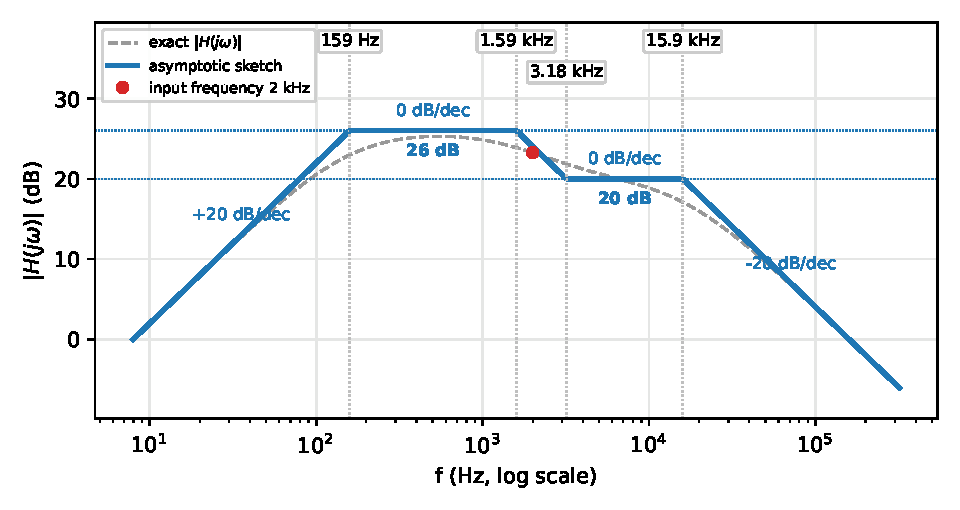
\includegraphics[width=0.78\linewidth,height=6.5cm,keepaspectratio]{p13_bode}\end{center}

{\small Blue: the straight-line sketch you are expected to draw. Dashed grey: the exact curve (about 3\,dB below the corner of an isolated pole). Red dot: the input frequency of Step 7.}
\solstep{7}{Steady-state output}The input is $V_i(t) = 0.01\sin\left(2\pi\cdot 2000\,t\right)$, so $\omega_{in} = 2\pi\cdot 2000 = 12600$\,rad/s. Put $s=j\omega_{in}$ in each factor (tool T5): magnitudes multiply, angles add.
{\small Rules: $\left|\frac{s}{s+p}\right| = \frac{\omega}{\sqrt{\omega^2+p^2}}$, $\angle = \frac{\pi}{2}-\tan^{-1}\frac{\omega}{p}$;\quad $\left|\frac{1}{1+s/p}\right| = \frac{1}{\sqrt{1+(\omega/p)^2}}$, $\angle = -\tan^{-1}\frac{\omega}{p}$;\quad $\left|1+\frac{s}{z}\right| = \sqrt{1+(\omega/z)^2}$, $\angle = \tan^{-1}\frac{\omega}{z}$;\quad a negative $K$ adds $-\pi$.}
\begin{center}\renewcommand{\arraystretch}{1.35}
\begin{tabular}{ccc}
\toprule
factor & magnitude & angle (rad) \\
\midrule
$20$ & $20$ & $0$ \\
$\rule[-1.1em]{0pt}{2.8em}\dfrac{s}{s+2\pi\cdot 159}$ & $0.9968$ & $0.0794$ \\
$\rule[-1.7em]{0pt}{4em}\dfrac{1}{1+\dfrac{s}{2\pi\cdot 1.59\mathrm{k}}}$ & $0.6227$ & $-0.899$ \\
$\rule[-1.1em]{0pt}{2.8em}\left(1+\dfrac{s}{2\pi\cdot 3.18\mathrm{k}}\right)$ & $1.181$ & $0.561$ \\
$\rule[-1.7em]{0pt}{4em}\dfrac{1}{1+\dfrac{s}{2\pi\cdot 15.9\mathrm{k}}}$ & $0.9922$ & $-0.125$ \\
\textbf{total} & $\mathbf{14.55}$ (product) & $\mathbf{-0.383}$ (sum) \\
\bottomrule
\end{tabular}\end{center}

\begin{align*}
|H(j\omega_{in})| &= 14.5, \qquad \angle H(j\omega_{in}) = -0.383\ \mathrm{rad} \\
v_{o,ac}(t) &= 14.5\times 0.01\,\sin\left(2\pi\cdot 2000\,t - 0.383\right) = 0.145\,\sin\left(2\pi\cdot 2000\,t - 0.383\right)
\end{align*}

\[
\boxed{V_o(t) = 0.145\,\sin\left(2\pi\cdot 2000\,t - 0.383\right)\ \mathrm{V}}
\]

\begin{ansbox}
$H(s) = 20\,\dfrac{s}{s+2\pi\cdot 159}\,\dfrac{1}{1+\dfrac{s}{2\pi\cdot 1.59\mathrm{k}}}\,\left(1+\dfrac{s}{2\pi\cdot 3.18\mathrm{k}}\right)\,\dfrac{1}{1+\dfrac{s}{2\pi\cdot 15.9\mathrm{k}}}$\quad (corners: 159 Hz, 1.59 kHz, 3.18 kHz, 15.9 kHz)\\[4pt]
$V_o(t) = 0.145\,\sin\left(2\pi\cdot 2000\,t - 0.383\right)\ \mathrm{V}$
\end{ansbox}

\newpage
\subsection*{Solution 2A.14 \hfill Hard}
\begin{center}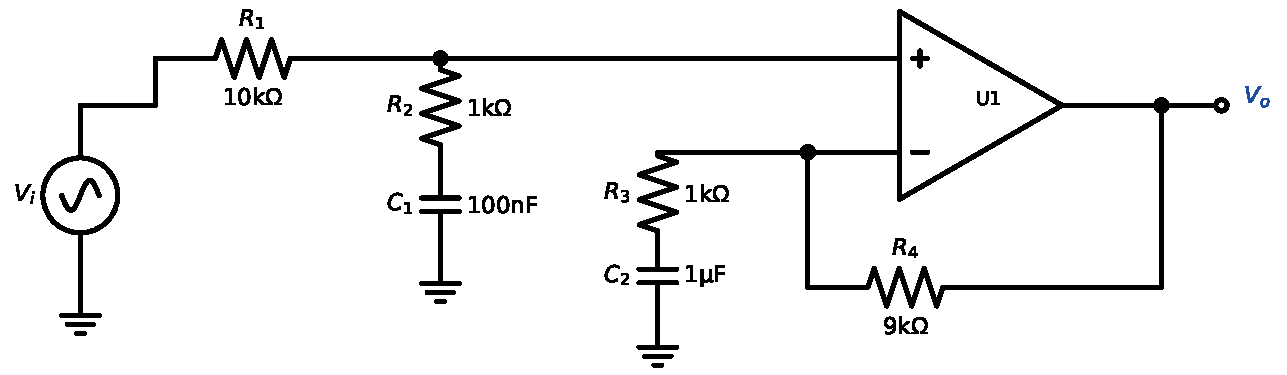
\includegraphics[width=\linewidth,height=5cm,keepaspectratio]{p14_circuit}\end{center}
\solstep{1}{Identify the sources}Independent sources: the AC input $V_i(t)$. No DC source: $V_{o,dc}=0$ and Step 2 is skipped.
\solstep{2}{DC circuit}No DC sources: $V_{o,dc}=0$.
\solstep{3}{Op-amp rules}The op-amp has negative feedback (its output is connected back to its $-$ input), so with an ideal op-amp (tool T1): (a) no current flows into the $+$ or $-$ input; (b) $V_-=V_+$ (virtual short). The circuit is a standard block, so use its block formula (tool T2).
\solstep{4}{Transfer function, block by block}\textbf{Block 1 (U1).} Non-inverting block: No current flows into the $+$ input, so $Z_{b1}$ and $R_{1}$ form a plain voltage divider: $V_+ = \frac{Z_{b1}}{R_{1} + Z_{b1}}V_{i}$. The op-amp forces $V_-=V_+$, and $Z_{g1}$, $R_{4}$ divide the output: $V_- = \frac{Z_{g1}}{Z_{g1} + R_{4}}V_{o}$, hence $V_{o} = \left(1+\frac{R_{4}}{Z_{g1}}\right)V_+$.\begin{align*}
Z_{b1} &= R_{2} + \frac{1}{sC_{1}} = \dfrac{1000\,s + 10^{7}}{s} \\
Z_{g1} &= R_{3} + \frac{1}{sC_{2}} = \dfrac{1000\,s + 10^{6}}{s}
\end{align*}
\[
\frac{V_{o}}{V_{i}} = \frac{Z_{b1}}{R_{1} + Z_{b1}}\left(1+\frac{R_{4}}{Z_{g1}}\right) = \dfrac{0.909\,s^{2} + 9180\,s + 9.09\times 10^{5}}{s^{2} + 1910\,s + 9.09\times 10^{5}}
\]

So:\[
H(s) = \dfrac{0.909\,s^{2} + 9180\,s + 9.09\times 10^{5}}{s^{2} + 1910\,s + 9.09\times 10^{5}}
\]

\solstep{5}{Standard (Bode-ready) form}Find the roots. Every root $s=-p$ of the denominator is a \emph{pole}, every root $s=-z$ of the numerator is a \emph{zero}; $|p|$ and $|z|$ are the corner frequencies (rad/s).
\begin{itemize}[leftmargin=*,itemsep=2pt]
\item Numerator: $0.909\,s^{2} + 9180\,s + 9.09\times 10^{5}$; divide by the leading coefficient $0.909$ (this does not move the roots): $s^{2} + 10100\,s + 10^{6}$; quadratic formula:\[
s = \frac{-10100 \pm \sqrt{(10100)^2 - 4(10^{6})}}{2} = \frac{-10100 \pm 9900}{2} \Rightarrow s = -100,\ -10000
\]

\item Denominator: $s^{2} + 1910\,s + 9.09\times 10^{5}$; quadratic formula:\[
s = \frac{-1910 \pm \sqrt{(1910)^2 - 4(9.09\times 10^{5})}}{2} = \frac{-1910 \pm 90.9}{2} \Rightarrow s = -909,\ -1000
\]

\end{itemize}

Factored form (leading coefficient in front):
\[
H(s) = 0.909\,\dfrac{(s+100)(s+10000)}{(s+909)(s+1000)}
\]

Bode-ready form: rewrite every $(s+p) = p\left(1+\frac{s}{p}\right)$ and $(s+z) = z\left(1+\frac{s}{z}\right)$, and collect all constants into $K$. Then every factor except $K$ is $\approx 1$ inside the pass-band:
\[
H(s) = 1\,\left(1+\dfrac{s}{2\pi\cdot 15.9}\right)\,\dfrac{1}{1+\dfrac{s}{2\pi\cdot 145}}\,\dfrac{1}{1+\dfrac{s}{2\pi\cdot 159}}\,\left(1+\dfrac{s}{2\pi\cdot 1.59\mathrm{k}}\right),\qquad K = 1
\]

\begin{center}\renewcommand{\arraystretch}{1.35}
\begin{tabular}{cccc}
\toprule
type & $\omega_c$ (rad/s) & $f_c=\omega_c/2\pi$ & slope change \\
\midrule
zero & $100$ & 15.9 Hz & $+20$ dB/dec \\
pole & $909$ & 145 Hz & $-20$ dB/dec \\
pole & $1000$ & 159 Hz & $-20$ dB/dec \\
zero & $10000$ & 1.59 kHz & $+20$ dB/dec \\
\bottomrule
\end{tabular}\end{center}

\solstep{6}{Magnitude Bode plot}Below every corner, all factors are $\approx$ constant: $|H| \approx 1$ $= -0.000000000000000964$\,dB (flat, 0 dB/dec). Then, moving right, each pole bends the line down by 20\,dB/dec and each zero bends it up by 20\,dB/dec (tool T6):
\begin{center}\renewcommand{\arraystretch}{1.35}
\begin{tabular}{lcl}
\toprule
frequency range & slope & asymptote level \\
\midrule
$f<$ 15.9 Hz & $0$ dB/dec (flat) & 0 dB at end \\
15.9 Hz -- 145 Hz & $+20$ dB/dec & 0 dB at start, 19.2 dB at end \\
145 Hz -- 159 Hz & $0$ dB/dec (flat) & 19.2 dB at start, 19.2 dB at end \\
159 Hz -- 1.59 kHz & $-20$ dB/dec & 19.2 dB at start, -0.828 dB at end \\
$f>$ 1.59 kHz & $0$ dB/dec (flat) & -0.828 dB at start \\
\bottomrule
\end{tabular}\end{center}

\begin{center}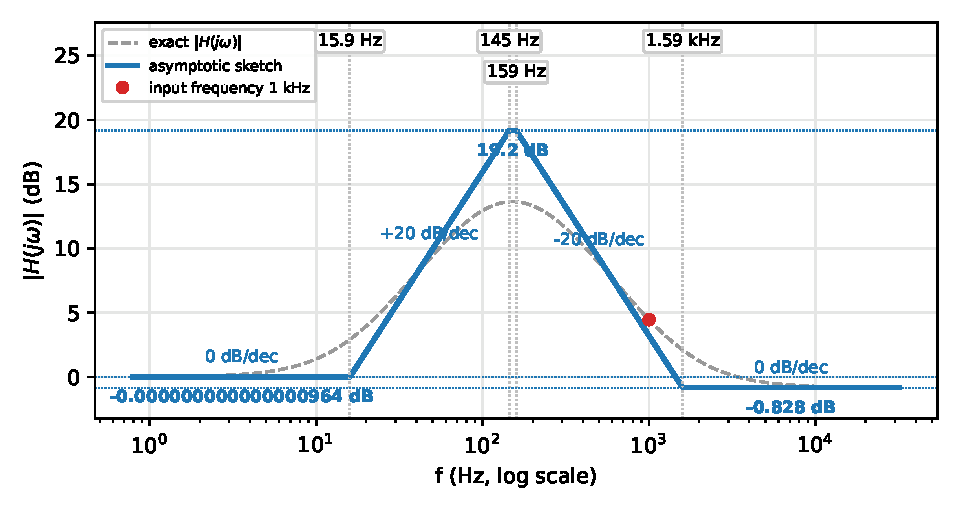
\includegraphics[width=0.78\linewidth,height=6.5cm,keepaspectratio]{p14_bode}\end{center}

{\small Blue: the straight-line sketch you are expected to draw. Dashed grey: the exact curve (about 3\,dB below the corner of an isolated pole). Red dot: the input frequency of Step 7.}
\solstep{7}{Steady-state output}The input is $V_i(t) = 0.1\sin\left(2\pi\cdot 1000\,t+\frac{\pi}{4}\right)$, so $\omega_{in} = 2\pi\cdot 1000 = 6280$\,rad/s. Put $s=j\omega_{in}$ in each factor (tool T5): magnitudes multiply, angles add.
{\small Rules: $\left|\frac{s}{s+p}\right| = \frac{\omega}{\sqrt{\omega^2+p^2}}$, $\angle = \frac{\pi}{2}-\tan^{-1}\frac{\omega}{p}$;\quad $\left|\frac{1}{1+s/p}\right| = \frac{1}{\sqrt{1+(\omega/p)^2}}$, $\angle = -\tan^{-1}\frac{\omega}{p}$;\quad $\left|1+\frac{s}{z}\right| = \sqrt{1+(\omega/z)^2}$, $\angle = \tan^{-1}\frac{\omega}{z}$;\quad a negative $K$ adds $-\pi$.}
\begin{center}\renewcommand{\arraystretch}{1.35}
\begin{tabular}{ccc}
\toprule
factor & magnitude & angle (rad) \\
\midrule
$1$ & $1$ & $0$ \\
$\rule[-1.1em]{0pt}{2.8em}\left(1+\dfrac{s}{2\pi\cdot 15.9}\right)$ & $62.84$ & $1.55$ \\
$\rule[-1.7em]{0pt}{4em}\dfrac{1}{1+\dfrac{s}{2\pi\cdot 145}}$ & $0.1432$ & $-1.43$ \\
$\rule[-1.7em]{0pt}{4em}\dfrac{1}{1+\dfrac{s}{2\pi\cdot 159}}$ & $0.1572$ & $-1.41$ \\
$\rule[-1.1em]{0pt}{2.8em}\left(1+\dfrac{s}{2\pi\cdot 1.59\mathrm{k}}\right)$ & $1.181$ & $0.561$ \\
\textbf{total} & $\mathbf{1.67}$ (product) & $\mathbf{-0.724}$ (sum) \\
\bottomrule
\end{tabular}\end{center}

\begin{align*}
|H(j\omega_{in})| &= 1.67, \qquad \angle H(j\omega_{in}) = -0.724\ \mathrm{rad} \\
v_{o,ac}(t) &= 1.67\times 0.1\,\sin\left(2\pi\cdot 1000\,t + 0.0612\right) = 0.167\,\sin\left(2\pi\cdot 1000\,t + 0.0612\right)
\end{align*}

(phase: $\theta + \angle H = \frac{\pi}{4} + (-0.724) = 0.0612$\,rad.)
\[
\boxed{V_o(t) = 0.167\,\sin\left(2\pi\cdot 1000\,t + 0.0612\right)\ \mathrm{V}}
\]

\begin{ansbox}
$H(s) = 1\,\left(1+\dfrac{s}{2\pi\cdot 15.9}\right)\,\dfrac{1}{1+\dfrac{s}{2\pi\cdot 145}}\,\dfrac{1}{1+\dfrac{s}{2\pi\cdot 159}}\,\left(1+\dfrac{s}{2\pi\cdot 1.59\mathrm{k}}\right)$\quad (corners: 15.9 Hz, 145 Hz, 159 Hz, 1.59 kHz)\\[4pt]
$V_o(t) = 0.167\,\sin\left(2\pi\cdot 1000\,t + 0.0612\right)\ \mathrm{V}$
\end{ansbox}

\newpage
\subsection*{Solution 2A.15 \hfill Hard}
\begin{center}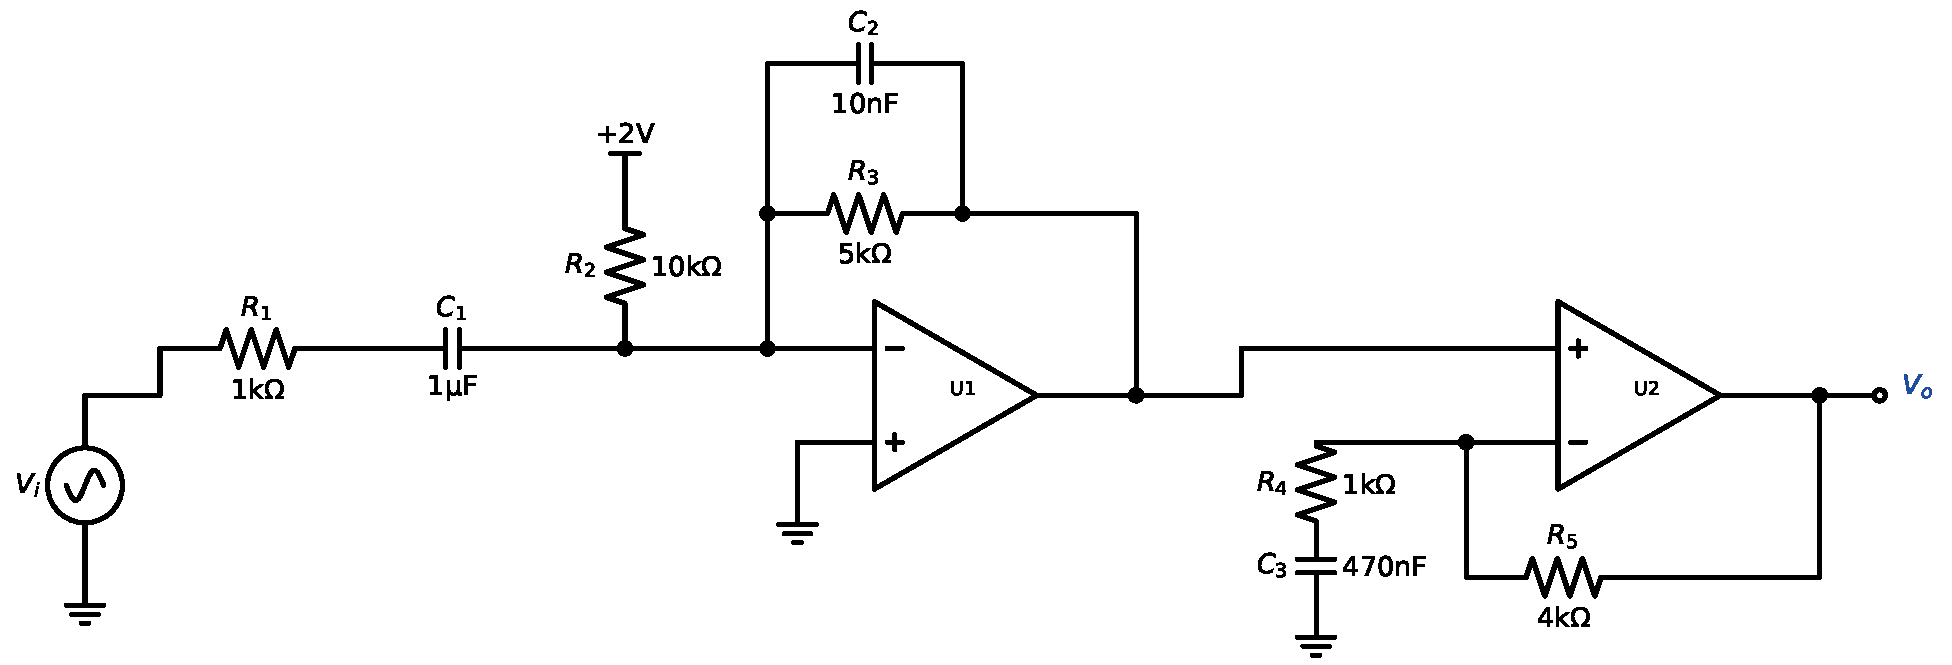
\includegraphics[width=\linewidth,height=5cm,keepaspectratio]{p15_circuit}\end{center}
\solstep{1}{Identify the sources}Independent sources: the AC input $V_i(t)$ and the DC supply $+2\,\mathrm{V}$. Both DC and AC are present, so use superposition: $V_o(t) = V_{o,dc}+v_{o,ac}(t)$. The DC part is Step 2, the AC part Steps 3--7.
\solstep{2}{DC circuit $\Rightarrow V_{o,dc}$}DC rules: $V_i=0$ and every capacitor is an open circuit (no inductors appear in these circuits). A block passes DC with its gain at $s=0$, i.e. $H_k(0)$.
\begin{enumerate}[leftmargin=*,itemsep=2pt]
\item Block 1 (summer): $Z_{in1}$ contains a capacitor, so it is open and carries no DC current. Only the supply drives a DC current, $\frac{V_{DC}}{R_{2}}$, through $Z_{f1}$ (at DC $R_{2}=10\,\mathrm{k}\Omega$, $Z_{f1}=5\,\mathrm{k}\Omega$):\[
V_{o1}\big|_{dc} = -Z_{f1}\frac{V_{DC}}{R_{2}} = -5\,\mathrm{k}\cdot\frac{2}{10\,\mathrm{k}} = -1\,\mathrm{V}
\]

\item Block 2: $H_2(0) = 1$ (capacitors open), so $V_{o}\big|_{dc} = 1\times (-1) = -1\,\mathrm{V}$.
\end{enumerate}

\[
\boxed{V_{o,dc} = -1\,\mathrm{V}}
\]

\solstep{3}{Op-amp rules}Each op-amp has negative feedback (its output is connected back to its $-$ input), so with an ideal op-amp (tool T1): (a) no current flows into the $+$ or $-$ input; (b) $V_-=V_+$ (virtual short). The circuit is a cascade of standard blocks, so each block is solved with its block formula (tool T2).
\solstep{4}{Transfer function, block by block}Each op-amp output is an ideal voltage source, so a block's output does not change when the next block is connected: the blocks can be solved one at a time and multiplied.\[
H(s) = \frac{V_o}{V_i} = \frac{V_{o1}}{V_{i}}\cdot\frac{V_{o}}{V_{o1}}
\]

\textbf{Block 1 (U1).} Summing block: $V_-=V_+=0$ (virtual ground), so the input currents $\frac{V_{i}}{Z_{in1}}$ and $\frac{V_{DC}}{R_{2}}$ simply add and both flow through $Z_{f1}$: $V_{o1} = -Z_{f1}\left(\frac{V_{i}}{Z_{in1}} + \frac{V_{DC}}{R_{2}}\right)$. For the AC part the supply is zero, so $R_{2}$ (from virtual ground to AC ground) carries no AC current and drops out.\begin{align*}
Z_{in1} &= R_{1} + \frac{1}{sC_{1}} = \dfrac{1000\,s + 10^{6}}{s} \\
Z_{f1} &= R_{3} \parallel \frac{1}{sC_{2}} = \dfrac{10^{8}}{s + 20000}
\end{align*}
\[
\frac{V_{o1}}{V_{i}} = -\frac{Z_{f1}}{Z_{in1}} = \dfrac{-10^{5}\,s}{s^{2} + 21000\,s + 2\times 10^{7}}
\]

\textbf{Block 2 (U2).} Non-inverting block: The $+$ input is the block input: $V_+ = V_{o1}$. The op-amp forces $V_-=V_+$, and $Z_{g2}$, $R_{5}$ divide the output: $V_- = \frac{Z_{g2}}{Z_{g2} + R_{5}}V_{o}$, hence $V_{o} = \left(1+\frac{R_{5}}{Z_{g2}}\right)V_+$.\begin{align*}
Z_{g2} &= R_{4} + \frac{1}{sC_{3}} = \dfrac{1000\,s + 2.13\times 10^{6}}{s}
\end{align*}
\[
\frac{V_{o}}{V_{o1}} = \left(1+\frac{R_{5}}{Z_{g2}}\right) = \dfrac{5\,s + 2130}{s + 2130}
\]

Multiply the blocks and simplify:\[
H(s) = \dfrac{-5\times 10^{5}\,s^{2} - 2.13\times 10^{8}\,s}{s^{3} + 23100\,s^{2} + 6.47\times 10^{7}\,s + 4.26\times 10^{10}}
\]

\solstep{5}{Standard (Bode-ready) form}Find the roots. Every root $s=-p$ of the denominator is a \emph{pole}, every root $s=-z$ of the numerator is a \emph{zero}; $|p|$ and $|z|$ are the corner frequencies (rad/s).
\begin{itemize}[leftmargin=*,itemsep=2pt]
\item Numerator: it has the factor $s$ $\Rightarrow$ 1 zero at $s=0$.
\item Numerator (after taking out the $s$ factor): $-5\times 10^{5}\,s - 2.13\times 10^{8}$; divide by the leading coefficient $-5\times 10^{5}$ (this does not move the roots): $s + 426$; $s + 426 = 0 \Rightarrow s = -426$.
\item Denominator: $s^{3} + 23100\,s^{2} + 6.47\times 10^{7}\,s + 4.26\times 10^{10}$; this is degree 3: use a calculator's polynomial solver (or \texttt{numpy.roots}) $\Rightarrow s = -1000,\ -2130,\ -20000$.
\end{itemize}

Factored form (leading coefficient in front):
\[
H(s) = -5\times 10^{5}\,\dfrac{s(s+426)}{(s+1000)(s+2130)(s+20000)}
\]

Bode-ready form: rewrite every $(s+p) = p\left(1+\frac{s}{p}\right)$ and $(s+z) = z\left(1+\frac{s}{z}\right)$, and collect all constants into $K$. Each $s$ in the numerator is paired with one of the \emph{lowest} poles as $\frac{s}{s+p}$ (that factor is $\approx 1$ above $p$). Then every factor except $K$ is $\approx 1$ inside the pass-band:
\[
H(s) = -5\,\dfrac{s}{s+2\pi\cdot 159}\,\left(1+\dfrac{s}{2\pi\cdot 67.7}\right)\,\dfrac{1}{1+\dfrac{s}{2\pi\cdot 339}}\,\dfrac{1}{1+\dfrac{s}{2\pi\cdot 3.18\mathrm{k}}},\qquad K = -5
\]

\begin{center}\renewcommand{\arraystretch}{1.35}
\begin{tabular}{cccc}
\toprule
type & $\omega_c$ (rad/s) & $f_c=\omega_c/2\pi$ & slope change \\
\midrule
zero & $426$ & 67.7 Hz & $+20$ dB/dec \\
pole & $1000$ & 159 Hz & $-20$ dB/dec \\
pole & $2130$ & 339 Hz & $-20$ dB/dec \\
pole & $20000$ & 3.18 kHz & $-20$ dB/dec \\
\bottomrule
\end{tabular}\end{center}

\solstep{6}{Magnitude Bode plot}Below every corner $|H(s)|\approx 0.005\,s$, so the plot starts with a slope of $+20$\,dB/dec. Then, moving right, each pole bends the line down by 20\,dB/dec and each zero bends it up by 20\,dB/dec (tool T6):
\begin{center}\renewcommand{\arraystretch}{1.35}
\begin{tabular}{lcl}
\toprule
frequency range & slope & asymptote level \\
\midrule
$f<$ 67.7 Hz & $+20$ dB/dec & 6.56 dB at end \\
67.7 Hz -- 159 Hz & $+40$ dB/dec & 6.56 dB at start, 21.4 dB at end \\
159 Hz -- 339 Hz & $+20$ dB/dec & 21.4 dB at start, 28 dB at end \\
339 Hz -- 3.18 kHz & $0$ dB/dec (flat) & 28 dB at start, 28 dB at end \\
$f>$ 3.18 kHz & $-20$ dB/dec & 28 dB at start \\
\bottomrule
\end{tabular}\end{center}

\begin{center}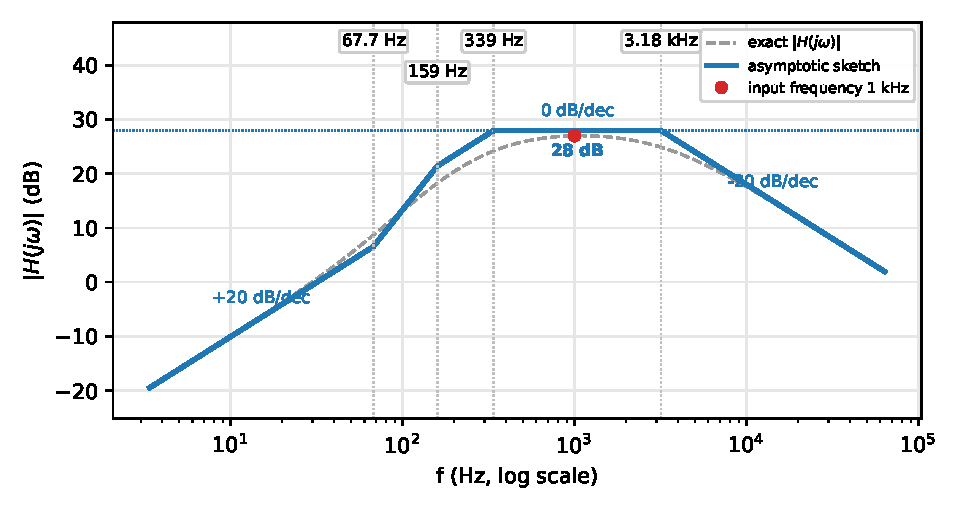
\includegraphics[width=0.78\linewidth,height=6.5cm,keepaspectratio]{p15_bode}\end{center}

{\small Blue: the straight-line sketch you are expected to draw. Dashed grey: the exact curve (about 3\,dB below the corner of an isolated pole). Red dot: the input frequency of Step 7.}
\solstep{7}{Steady-state output}The input is $V_i(t) = 0.05\sin\left(2\pi\cdot 1000\,t\right)$, so $\omega_{in} = 2\pi\cdot 1000 = 6280$\,rad/s. Put $s=j\omega_{in}$ in each factor (tool T5): magnitudes multiply, angles add.
{\small Rules: $\left|\frac{s}{s+p}\right| = \frac{\omega}{\sqrt{\omega^2+p^2}}$, $\angle = \frac{\pi}{2}-\tan^{-1}\frac{\omega}{p}$;\quad $\left|\frac{1}{1+s/p}\right| = \frac{1}{\sqrt{1+(\omega/p)^2}}$, $\angle = -\tan^{-1}\frac{\omega}{p}$;\quad $\left|1+\frac{s}{z}\right| = \sqrt{1+(\omega/z)^2}$, $\angle = \tan^{-1}\frac{\omega}{z}$;\quad a negative $K$ adds $-\pi$.}
\begin{center}\renewcommand{\arraystretch}{1.35}
\begin{tabular}{ccc}
\toprule
factor & magnitude & angle (rad) \\
\midrule
$-5$ & $5$ & $-3.14$ \\
$\rule[-1.1em]{0pt}{2.8em}\dfrac{s}{s+2\pi\cdot 159}$ & $0.9876$ & $0.158$ \\
$\rule[-1.1em]{0pt}{2.8em}\left(1+\dfrac{s}{2\pi\cdot 67.7}\right)$ & $14.8$ & $1.5$ \\
$\rule[-1.7em]{0pt}{4em}\dfrac{1}{1+\dfrac{s}{2\pi\cdot 339}}$ & $0.3207$ & $-1.24$ \\
$\rule[-1.7em]{0pt}{4em}\dfrac{1}{1+\dfrac{s}{2\pi\cdot 3.18\mathrm{k}}}$ & $0.954$ & $-0.304$ \\
\textbf{total} & $\mathbf{22.36}$ (product) & $\mathbf{-3.03}$ (sum) \\
\bottomrule
\end{tabular}\end{center}

\begin{align*}
|H(j\omega_{in})| &= 22.4, \qquad \angle H(j\omega_{in}) = -3.03\ \mathrm{rad} \\
v_{o,ac}(t) &= 22.4\times 0.05\,\sin\left(2\pi\cdot 1000\,t - 3.03\right) = 1.12\,\sin\left(2\pi\cdot 1000\,t - 3.03\right)
\end{align*}

Add the DC part from Step 2 (superposition):
\[
\boxed{V_o(t) = -1 + 1.12\,\sin\left(2\pi\cdot 1000\,t - 3.03\right)\ \mathrm{V}}
\]

\begin{ansbox}
$H(s) = -5\,\dfrac{s}{s+2\pi\cdot 159}\,\left(1+\dfrac{s}{2\pi\cdot 67.7}\right)\,\dfrac{1}{1+\dfrac{s}{2\pi\cdot 339}}\,\dfrac{1}{1+\dfrac{s}{2\pi\cdot 3.18\mathrm{k}}}$\quad (corners: 67.7 Hz, 159 Hz, 339 Hz, 3.18 kHz)\\[4pt]
$V_o(t) = -1 + 1.12\,\sin\left(2\pi\cdot 1000\,t - 3.03\right)\ \mathrm{V}$
\end{ansbox}

\newpage
\subsection*{Solution 2A.16 \hfill Hard}
\begin{center}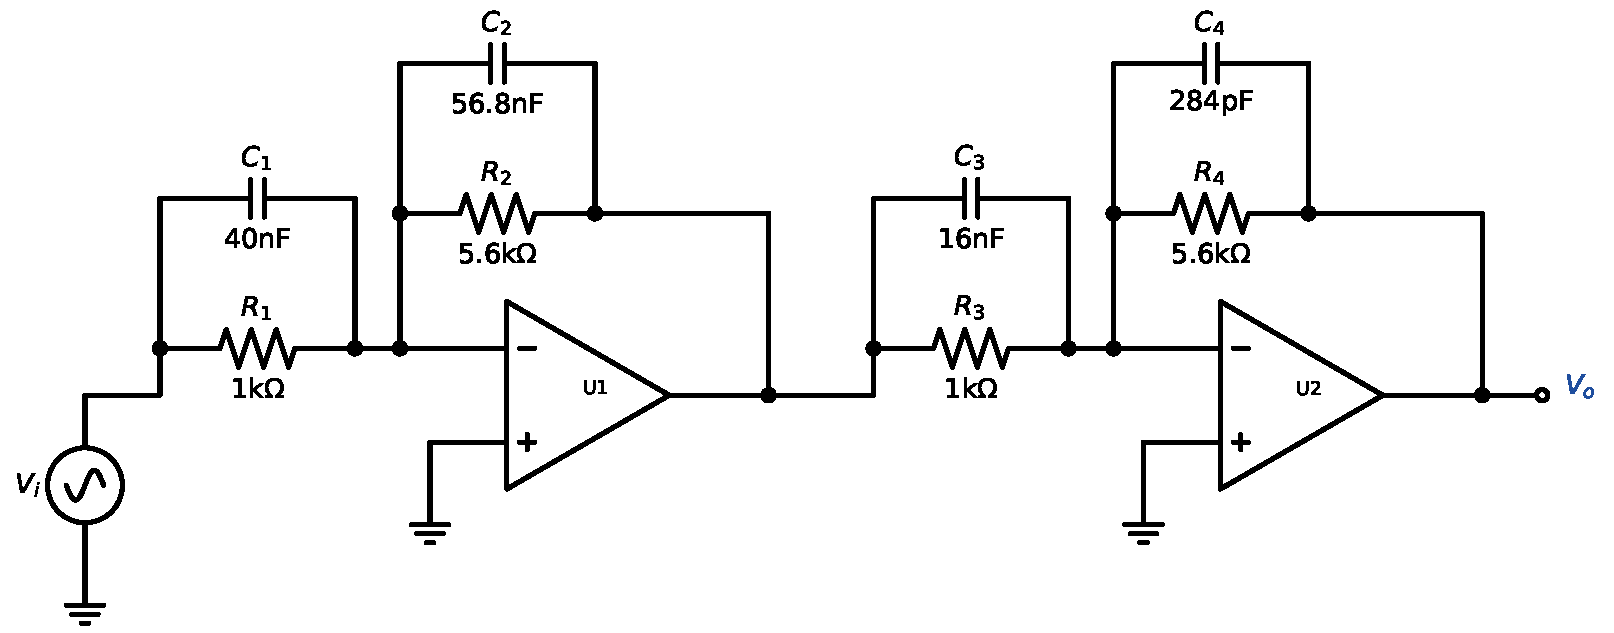
\includegraphics[width=\linewidth,height=5cm,keepaspectratio]{p16_circuit}\end{center}
\solstep{1}{Identify the sources}Independent sources: the AC input $V_i(t)$. No DC source: $V_{o,dc}=0$ and Step 2 is skipped.
\solstep{2}{DC circuit}No DC sources: $V_{o,dc}=0$.
\solstep{3}{Op-amp rules}Each op-amp has negative feedback (its output is connected back to its $-$ input), so with an ideal op-amp (tool T1): (a) no current flows into the $+$ or $-$ input; (b) $V_-=V_+$ (virtual short). The circuit is a cascade of standard blocks, so each block is solved with its block formula (tool T2).
\solstep{4}{Transfer function, block by block}Each op-amp output is an ideal voltage source, so a block's output does not change when the next block is connected: the blocks can be solved one at a time and multiplied.\[
H(s) = \frac{V_o}{V_i} = \frac{V_{o1}}{V_{i}}\cdot\frac{V_{o}}{V_{o1}}
\]

\textbf{Block 1 (U1).} Inverting block: the $+$ input is grounded, so $V_- = V_+ = 0$ (virtual ground). The current $\frac{V_{i} - 0}{Z_{in1}}$ through $Z_{in1}$ cannot enter the op-amp, so all of it flows through $Z_{f1}$: $V_{o1} = 0 - Z_{f1}\cdot\frac{V_{i}}{Z_{in1}}$.\begin{align*}
Z_{in1} &= R_{1} \parallel \frac{1}{sC_{1}} = \dfrac{2.5\times 10^{7}}{s + 25000} \\
Z_{f1} &= R_{2} \parallel \frac{1}{sC_{2}} = \dfrac{1.76\times 10^{7}}{s + 3140}
\end{align*}
\[
\frac{V_{o1}}{V_{i}} = -\frac{Z_{f1}}{Z_{in1}} = \dfrac{-0.704\,s - 17600}{s + 3140}
\]

\textbf{Block 2 (U2).} Inverting block: the $+$ input is grounded, so $V_- = V_+ = 0$ (virtual ground). The current $\frac{V_{o1} - 0}{Z_{in2}}$ through $Z_{in2}$ cannot enter the op-amp, so all of it flows through $Z_{f2}$: $V_{o} = 0 - Z_{f2}\cdot\frac{V_{o1}}{Z_{in2}}$.\begin{align*}
Z_{in2} &= R_{3} \parallel \frac{1}{sC_{3}} = \dfrac{6.25\times 10^{7}}{s + 62500} \\
Z_{f2} &= R_{4} \parallel \frac{1}{sC_{4}} = \dfrac{3.52\times 10^{9}}{s + 6.29\times 10^{5}}
\end{align*}
\[
\frac{V_{o}}{V_{o1}} = -\frac{Z_{f2}}{Z_{in2}} = \dfrac{-56.3\,s - 3.52\times 10^{6}}{s + 6.29\times 10^{5}}
\]

Multiply the blocks and simplify:\[
H(s) = \dfrac{39.7\,s^{2} + 3.47\times 10^{6}\,s + 6.2\times 10^{10}}{s^{2} + 6.32\times 10^{5}\,s + 1.98\times 10^{9}}
\]

\solstep{5}{Standard (Bode-ready) form}Find the roots. Every root $s=-p$ of the denominator is a \emph{pole}, every root $s=-z$ of the numerator is a \emph{zero}; $|p|$ and $|z|$ are the corner frequencies (rad/s).
\begin{itemize}[leftmargin=*,itemsep=2pt]
\item Numerator: $39.7\,s^{2} + 3.47\times 10^{6}\,s + 6.2\times 10^{10}$; divide by the leading coefficient $39.7$ (this does not move the roots): $s^{2} + 87500\,s + 1.56\times 10^{9}$; quadratic formula:\[
s = \frac{-87500 \pm \sqrt{(87500)^2 - 4(1.56\times 10^{9})}}{2} = \frac{-87500 \pm 37500}{2} \Rightarrow s = -25000,\ -62500
\]

\item Denominator: $s^{2} + 6.32\times 10^{5}\,s + 1.98\times 10^{9}$; quadratic formula:\[
s = \frac{-6.32\times 10^{5} \pm \sqrt{(6.32\times 10^{5})^2 - 4(1.98\times 10^{9})}}{2} = \frac{-6.32\times 10^{5} \pm 6.26\times 10^{5}}{2} \Rightarrow s = -3140,\ -6.29\times 10^{5}
\]

\end{itemize}

Factored form (leading coefficient in front):
\[
H(s) = 39.7\,\dfrac{(s+25000)(s+62500)}{(s+3140)(s+6.29\times 10^{5})}
\]

Bode-ready form: rewrite every $(s+p) = p\left(1+\frac{s}{p}\right)$ and $(s+z) = z\left(1+\frac{s}{z}\right)$, and collect all constants into $K$. Then every factor except $K$ is $\approx 1$ inside the pass-band:
\[
H(s) = 31.4\,\dfrac{1}{1+\dfrac{s}{2\pi\cdot 500}}\,\left(1+\dfrac{s}{2\pi\cdot 3.98\mathrm{k}}\right)\,\left(1+\dfrac{s}{2\pi\cdot 9.95\mathrm{k}}\right)\,\dfrac{1}{1+\dfrac{s}{2\pi\cdot 100\mathrm{k}}},\qquad K = 31.4
\]

\begin{center}\renewcommand{\arraystretch}{1.35}
\begin{tabular}{cccc}
\toprule
type & $\omega_c$ (rad/s) & $f_c=\omega_c/2\pi$ & slope change \\
\midrule
pole & $3140$ & 500 Hz & $-20$ dB/dec \\
zero & $25000$ & 3.98 kHz & $+20$ dB/dec \\
zero & $62500$ & 9.95 kHz & $+20$ dB/dec \\
pole & $6.29\times 10^{5}$ & 100 kHz & $-20$ dB/dec \\
\bottomrule
\end{tabular}\end{center}

\solstep{6}{Magnitude Bode plot}Below every corner, all factors are $\approx$ constant: $|H| \approx 31.4$ $= 29.9$\,dB (flat, 0 dB/dec). Then, moving right, each pole bends the line down by 20\,dB/dec and each zero bends it up by 20\,dB/dec (tool T6):
\begin{center}\renewcommand{\arraystretch}{1.35}
\begin{tabular}{lcl}
\toprule
frequency range & slope & asymptote level \\
\midrule
$f<$ 500 Hz & $0$ dB/dec (flat) & 29.9 dB at end \\
500 Hz -- 3.98 kHz & $-20$ dB/dec & 29.9 dB at start, 11.9 dB at end \\
3.98 kHz -- 9.95 kHz & $0$ dB/dec (flat) & 11.9 dB at start, 11.9 dB at end \\
9.95 kHz -- 100 kHz & $+20$ dB/dec & 11.9 dB at start, 32 dB at end \\
$f>$ 100 kHz & $0$ dB/dec (flat) & 32 dB at start \\
\bottomrule
\end{tabular}\end{center}

\begin{center}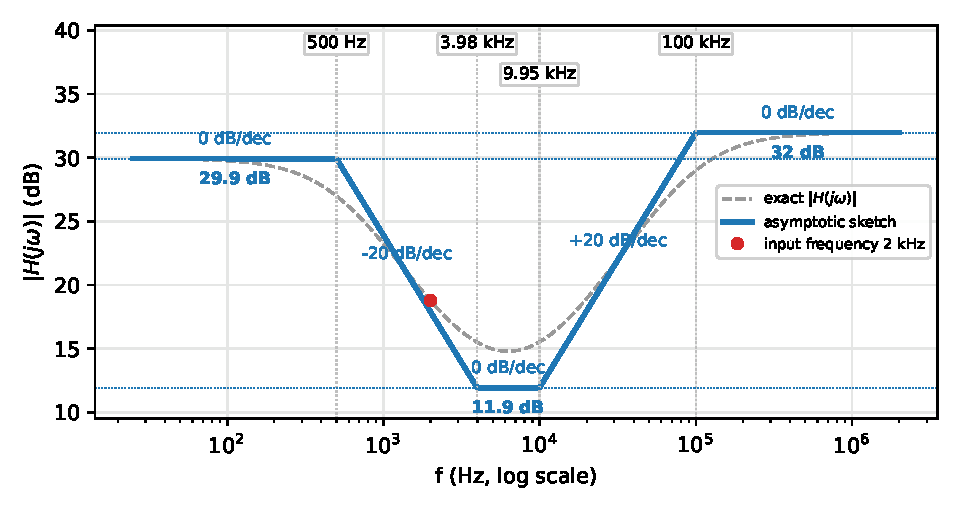
\includegraphics[width=0.78\linewidth,height=6.5cm,keepaspectratio]{p16_bode}\end{center}

{\small Blue: the straight-line sketch you are expected to draw. Dashed grey: the exact curve (about 3\,dB below the corner of an isolated pole). Red dot: the input frequency of Step 7.}
\solstep{7}{Steady-state output}The input is $V_i(t) = 0.01\sin\left(2\pi\cdot 2000\,t\right)$, so $\omega_{in} = 2\pi\cdot 2000 = 12600$\,rad/s. Put $s=j\omega_{in}$ in each factor (tool T5): magnitudes multiply, angles add.
{\small Rules: $\left|\frac{s}{s+p}\right| = \frac{\omega}{\sqrt{\omega^2+p^2}}$, $\angle = \frac{\pi}{2}-\tan^{-1}\frac{\omega}{p}$;\quad $\left|\frac{1}{1+s/p}\right| = \frac{1}{\sqrt{1+(\omega/p)^2}}$, $\angle = -\tan^{-1}\frac{\omega}{p}$;\quad $\left|1+\frac{s}{z}\right| = \sqrt{1+(\omega/z)^2}$, $\angle = \tan^{-1}\frac{\omega}{z}$;\quad a negative $K$ adds $-\pi$.}
\begin{center}\renewcommand{\arraystretch}{1.35}
\begin{tabular}{ccc}
\toprule
factor & magnitude & angle (rad) \\
\midrule
$31.4$ & $31.36$ & $0$ \\
$\rule[-1.7em]{0pt}{4em}\dfrac{1}{1+\dfrac{s}{2\pi\cdot 500}}$ & $0.2427$ & $-1.33$ \\
$\rule[-1.1em]{0pt}{2.8em}\left(1+\dfrac{s}{2\pi\cdot 3.98\mathrm{k}}\right)$ & $1.119$ & $0.466$ \\
$\rule[-1.1em]{0pt}{2.8em}\left(1+\dfrac{s}{2\pi\cdot 9.95\mathrm{k}}\right)$ & $1.02$ & $0.198$ \\
$\rule[-1.7em]{0pt}{4em}\dfrac{1}{1+\dfrac{s}{2\pi\cdot 100\mathrm{k}}}$ & $0.9998$ & $-0.02$ \\
\textbf{total} & $\mathbf{8.687}$ (product) & $\mathbf{-0.681}$ (sum) \\
\bottomrule
\end{tabular}\end{center}

\begin{align*}
|H(j\omega_{in})| &= 8.69, \qquad \angle H(j\omega_{in}) = -0.681\ \mathrm{rad} \\
v_{o,ac}(t) &= 8.69\times 0.01\,\sin\left(2\pi\cdot 2000\,t - 0.681\right) = 0.0869\,\sin\left(2\pi\cdot 2000\,t - 0.681\right)
\end{align*}

\[
\boxed{V_o(t) = 0.0869\,\sin\left(2\pi\cdot 2000\,t - 0.681\right)\ \mathrm{V}}
\]

\begin{ansbox}
$H(s) = 31.4\,\dfrac{1}{1+\dfrac{s}{2\pi\cdot 500}}\,\left(1+\dfrac{s}{2\pi\cdot 3.98\mathrm{k}}\right)\,\left(1+\dfrac{s}{2\pi\cdot 9.95\mathrm{k}}\right)\,\dfrac{1}{1+\dfrac{s}{2\pi\cdot 100\mathrm{k}}}$\quad (corners: 500 Hz, 3.98 kHz, 9.95 kHz, 100 kHz)\\[4pt]
$V_o(t) = 0.0869\,\sin\left(2\pi\cdot 2000\,t - 0.681\right)\ \mathrm{V}$
\end{ansbox}

\newpage
\subsection*{Solution 2A.17 \hfill Hard}
\begin{center}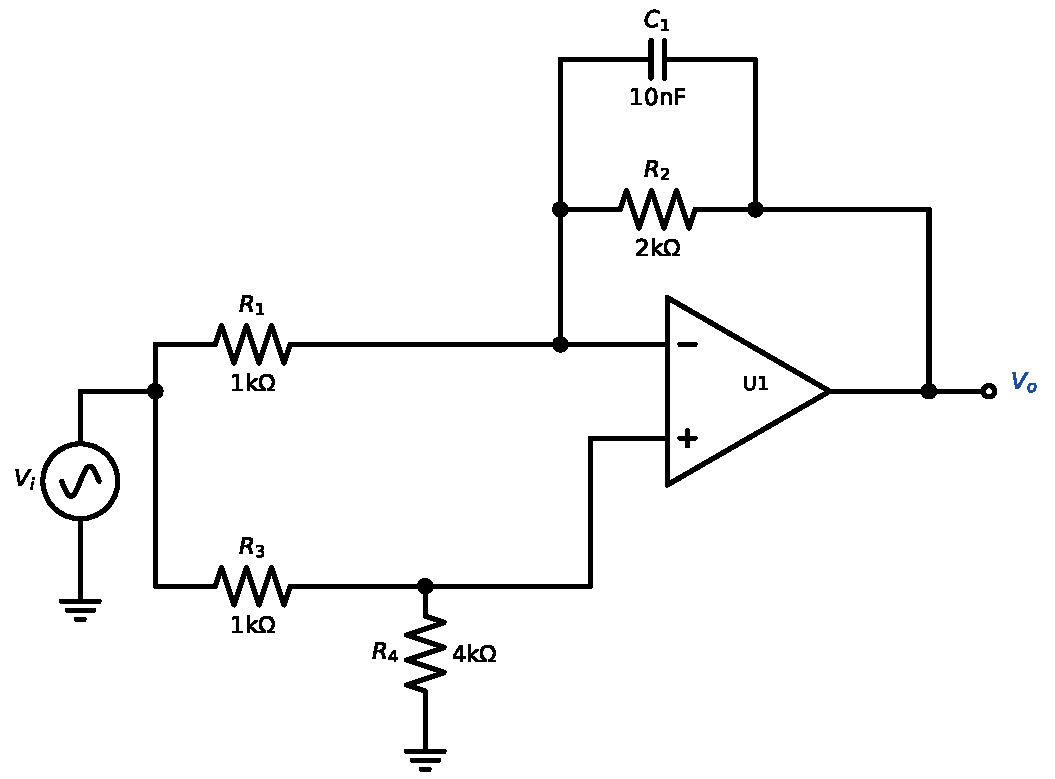
\includegraphics[width=\linewidth,height=5cm,keepaspectratio]{p17_circuit}\end{center}
\solstep{1}{Identify the sources}Independent sources: the AC input $V_i(t)$. No DC source: $V_{o,dc}=0$ and Step 2 is skipped.
\solstep{2}{DC circuit}No DC sources: $V_{o,dc}=0$.
\solstep{3}{Op-amp rules}The op-amp has negative feedback (its output is connected back to its $-$ input), so with an ideal op-amp (tool T1): (a) no current flows into the $+$ or $-$ input; (b) $V_-=V_+$ (virtual short). The circuit is a standard block, so use its block formula (tool T2).
\solstep{4}{Transfer function, block by block}\textbf{Block 1 (U1).} Difference block (both inputs driven by $V_{i}$): use superposition. Through the $+$ path the signal is divided, $V_+ = \frac{R_{4}}{R_{3}+R_{4}}V_{i}$, and amplified by the non-inverting gain $1+\frac{Z_{f1}}{R_{1}}$; through the $-$ path it is amplified by the inverting gain $-\frac{Z_{f1}}{R_{1}}$. Add the two contributions.\begin{align*}
Z_{f1} &= R_{2} \parallel \frac{1}{sC_{1}} = \dfrac{10^{8}}{s + 50000}
\end{align*}
\[
\frac{V_{o}}{V_{i}} = \frac{R_{4}}{R_{3}+R_{4}}\left(1+\frac{Z_{f1}}{R_{1}}\right) - \frac{Z_{f1}}{R_{1}} = \dfrac{0.8\,s + 20000}{s + 50000}
\]

So:\[
H(s) = \dfrac{0.8\,s + 20000}{s + 50000}
\]

\solstep{5}{Standard (Bode-ready) form}Find the roots. Every root $s=-p$ of the denominator is a \emph{pole}, every root $s=-z$ of the numerator is a \emph{zero}; $|p|$ and $|z|$ are the corner frequencies (rad/s).
\begin{itemize}[leftmargin=*,itemsep=2pt]
\item Numerator: $0.8\,s + 20000$; divide by the leading coefficient $0.8$ (this does not move the roots): $s + 25000$; $s + 25000 = 0 \Rightarrow s = -25000$.
\item Denominator: $s + 50000$; $s + 50000 = 0 \Rightarrow s = -50000$.
\end{itemize}

Factored form (leading coefficient in front):
\[
H(s) = 0.8\,\dfrac{(s+25000)}{(s+50000)}
\]

Bode-ready form: rewrite every $(s+p) = p\left(1+\frac{s}{p}\right)$ and $(s+z) = z\left(1+\frac{s}{z}\right)$, and collect all constants into $K$. Then every factor except $K$ is $\approx 1$ inside the pass-band:
\[
H(s) = 0.4\,\left(1+\dfrac{s}{2\pi\cdot 3.98\mathrm{k}}\right)\,\dfrac{1}{1+\dfrac{s}{2\pi\cdot 7.96\mathrm{k}}},\qquad K = 0.4
\]

\begin{center}\renewcommand{\arraystretch}{1.35}
\begin{tabular}{cccc}
\toprule
type & $\omega_c$ (rad/s) & $f_c=\omega_c/2\pi$ & slope change \\
\midrule
zero & $25000$ & 3.98 kHz & $+20$ dB/dec \\
pole & $50000$ & 7.96 kHz & $-20$ dB/dec \\
\bottomrule
\end{tabular}\end{center}

\solstep{6}{Magnitude Bode plot}Below every corner, all factors are $\approx$ constant: $|H| \approx 0.4$ $= -7.96$\,dB (flat, 0 dB/dec). Then, moving right, each pole bends the line down by 20\,dB/dec and each zero bends it up by 20\,dB/dec (tool T6):
\begin{center}\renewcommand{\arraystretch}{1.35}
\begin{tabular}{lcl}
\toprule
frequency range & slope & asymptote level \\
\midrule
$f<$ 3.98 kHz & $0$ dB/dec (flat) & -7.96 dB at end \\
3.98 kHz -- 7.96 kHz & $+20$ dB/dec & -7.96 dB at start, -1.94 dB at end \\
$f>$ 7.96 kHz & $0$ dB/dec (flat) & -1.94 dB at start \\
\bottomrule
\end{tabular}\end{center}

\begin{center}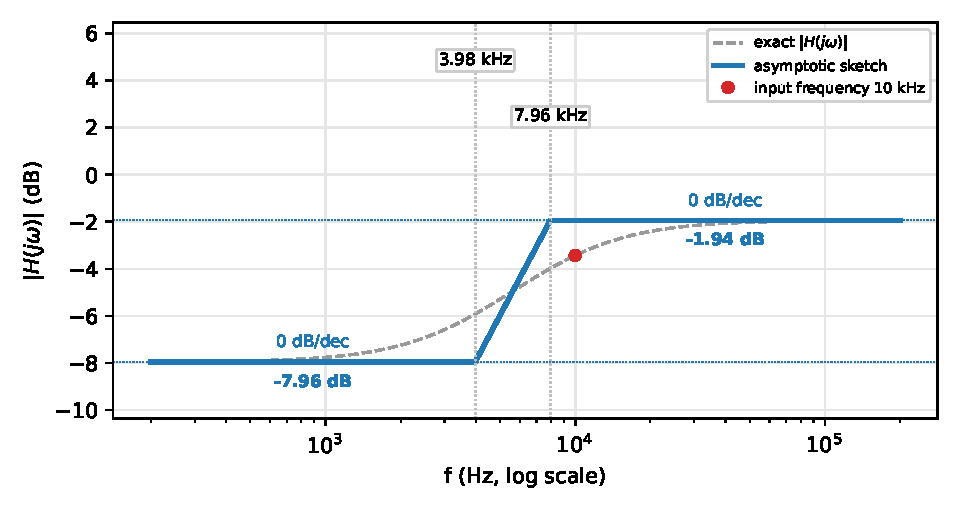
\includegraphics[width=0.78\linewidth,height=6.5cm,keepaspectratio]{p17_bode}\end{center}

{\small Blue: the straight-line sketch you are expected to draw. Dashed grey: the exact curve (about 3\,dB below the corner of an isolated pole). Red dot: the input frequency of Step 7.}
\solstep{7}{Steady-state output}The input is $V_i(t) = 0.5\cos\left(2\pi\cdot 10000\,t-\frac{\pi}{3}\right)$, so $\omega_{in} = 2\pi\cdot 10000 = 62800$\,rad/s. Put $s=j\omega_{in}$ in each factor (tool T5): magnitudes multiply, angles add.
{\small Rules: $\left|\frac{s}{s+p}\right| = \frac{\omega}{\sqrt{\omega^2+p^2}}$, $\angle = \frac{\pi}{2}-\tan^{-1}\frac{\omega}{p}$;\quad $\left|\frac{1}{1+s/p}\right| = \frac{1}{\sqrt{1+(\omega/p)^2}}$, $\angle = -\tan^{-1}\frac{\omega}{p}$;\quad $\left|1+\frac{s}{z}\right| = \sqrt{1+(\omega/z)^2}$, $\angle = \tan^{-1}\frac{\omega}{z}$;\quad a negative $K$ adds $-\pi$.}
\begin{center}\renewcommand{\arraystretch}{1.35}
\begin{tabular}{ccc}
\toprule
factor & magnitude & angle (rad) \\
\midrule
$0.4$ & $0.4$ & $0$ \\
$\rule[-1.1em]{0pt}{2.8em}\left(1+\dfrac{s}{2\pi\cdot 3.98\mathrm{k}}\right)$ & $2.705$ & $1.19$ \\
$\rule[-1.7em]{0pt}{4em}\dfrac{1}{1+\dfrac{s}{2\pi\cdot 7.96\mathrm{k}}}$ & $0.6227$ & $-0.899$ \\
\textbf{total} & $\mathbf{0.6737}$ (product) & $\mathbf{0.293}$ (sum) \\
\bottomrule
\end{tabular}\end{center}

\begin{align*}
|H(j\omega_{in})| &= 0.674, \qquad \angle H(j\omega_{in}) = 0.293\ \mathrm{rad} \\
v_{o,ac}(t) &= 0.674\times 0.5\,\cos\left(2\pi\cdot 10000\,t - 0.754\right) = 0.337\,\cos\left(2\pi\cdot 10000\,t - 0.754\right)
\end{align*}

(phase: $\theta + \angle H = -\frac{\pi}{3} + (0.293) = -0.754$\,rad.)
\[
\boxed{V_o(t) = 0.337\,\cos\left(2\pi\cdot 10000\,t - 0.754\right)\ \mathrm{V}}
\]

\begin{ansbox}
$H(s) = 0.4\,\left(1+\dfrac{s}{2\pi\cdot 3.98\mathrm{k}}\right)\,\dfrac{1}{1+\dfrac{s}{2\pi\cdot 7.96\mathrm{k}}}$\quad (corners: 3.98 kHz, 7.96 kHz)\\[4pt]
$V_o(t) = 0.337\,\cos\left(2\pi\cdot 10000\,t - 0.754\right)\ \mathrm{V}$
\end{ansbox}

\newpage
\subsection*{Solution 2A.18 \hfill Hard}
\begin{center}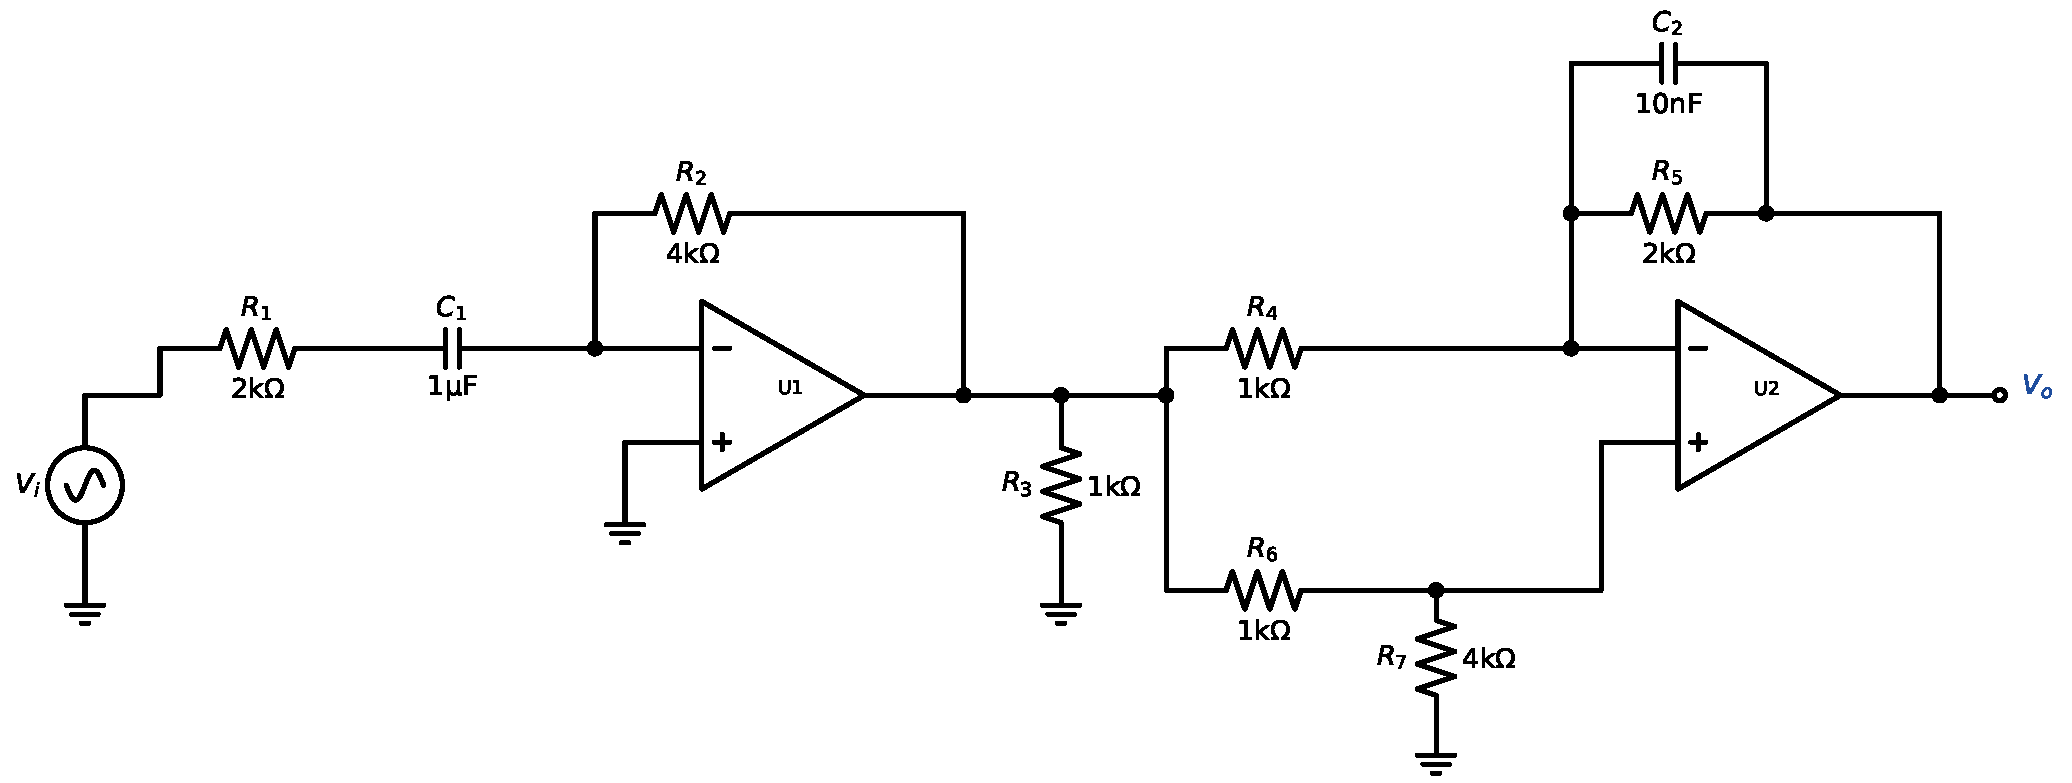
\includegraphics[width=\linewidth,height=5cm,keepaspectratio]{p18_circuit}\end{center}
\solstep{1}{Identify the sources}Independent sources: the AC input $V_i(t)$. No DC source: $V_{o,dc}=0$ and Step 2 is skipped.
\solstep{2}{DC circuit}No DC sources: $V_{o,dc}=0$.
\solstep{3}{Op-amp rules}Each op-amp has negative feedback (its output is connected back to its $-$ input), so with an ideal op-amp (tool T1): (a) no current flows into the $+$ or $-$ input; (b) $V_-=V_+$ (virtual short). The circuit is a cascade of standard blocks, so each block is solved with its block formula (tool T2).
\solstep{4}{Transfer function, block by block}Each op-amp output is an ideal voltage source, so a block's output does not change when the next block is connected: the blocks can be solved one at a time and multiplied.\[
H(s) = \frac{V_o}{V_i} = \frac{V_{o1}}{V_{i}}\cdot\frac{V_{o}}{V_{o1}}
\]

The load $R_{3}$ hangs on an op-amp output (an ideal voltage source): it draws current but does not change the output voltage, so it drops out of $H(s)$.
\textbf{Block 1 (U1).} Inverting block: the $+$ input is grounded, so $V_- = V_+ = 0$ (virtual ground). The current $\frac{V_{i} - 0}{Z_{in1}}$ through $Z_{in1}$ cannot enter the op-amp, so all of it flows through $R_{2}$: $V_{o1} = 0 - R_{2}\cdot\frac{V_{i}}{Z_{in1}}$.\begin{align*}
Z_{in1} &= R_{1} + \frac{1}{sC_{1}} = \dfrac{2000\,s + 10^{6}}{s}
\end{align*}
\[
\frac{V_{o1}}{V_{i}} = -\frac{R_{2}}{Z_{in1}} = \dfrac{-2\,s}{s + 500}
\]

\textbf{Block 2 (U2).} Difference block (both inputs driven by $V_{o1}$): use superposition. Through the $+$ path the signal is divided, $V_+ = \frac{R_{7}}{R_{6}+R_{7}}V_{o1}$, and amplified by the non-inverting gain $1+\frac{Z_{f2}}{R_{4}}$; through the $-$ path it is amplified by the inverting gain $-\frac{Z_{f2}}{R_{4}}$. Add the two contributions.\begin{align*}
Z_{f2} &= R_{5} \parallel \frac{1}{sC_{2}} = \dfrac{10^{8}}{s + 50000}
\end{align*}
\[
\frac{V_{o}}{V_{o1}} = \frac{R_{7}}{R_{6}+R_{7}}\left(1+\frac{Z_{f2}}{R_{4}}\right) - \frac{Z_{f2}}{R_{4}} = \dfrac{0.8\,s + 20000}{s + 50000}
\]

Multiply the blocks and simplify:\[
H(s) = \dfrac{-1.6\,s^{2} - 40000\,s}{s^{2} + 50500\,s + 2.5\times 10^{7}}
\]

\solstep{5}{Standard (Bode-ready) form}Find the roots. Every root $s=-p$ of the denominator is a \emph{pole}, every root $s=-z$ of the numerator is a \emph{zero}; $|p|$ and $|z|$ are the corner frequencies (rad/s).
\begin{itemize}[leftmargin=*,itemsep=2pt]
\item Numerator: it has the factor $s$ $\Rightarrow$ 1 zero at $s=0$.
\item Numerator (after taking out the $s$ factor): $-1.6\,s - 40000$; divide by the leading coefficient $-1.6$ (this does not move the roots): $s + 25000$; $s + 25000 = 0 \Rightarrow s = -25000$.
\item Denominator: $s^{2} + 50500\,s + 2.5\times 10^{7}$; quadratic formula:\[
s = \frac{-50500 \pm \sqrt{(50500)^2 - 4(2.5\times 10^{7})}}{2} = \frac{-50500 \pm 49500}{2} \Rightarrow s = -500,\ -50000
\]

\end{itemize}

Factored form (leading coefficient in front):
\[
H(s) = -1.6\,\dfrac{s(s+25000)}{(s+500)(s+50000)}
\]

Bode-ready form: rewrite every $(s+p) = p\left(1+\frac{s}{p}\right)$ and $(s+z) = z\left(1+\frac{s}{z}\right)$, and collect all constants into $K$. Each $s$ in the numerator is paired with one of the \emph{lowest} poles as $\frac{s}{s+p}$ (that factor is $\approx 1$ above $p$). Then every factor except $K$ is $\approx 1$ inside the pass-band:
\[
H(s) = -0.8\,\dfrac{s}{s+2\pi\cdot 79.6}\,\left(1+\dfrac{s}{2\pi\cdot 3.98\mathrm{k}}\right)\,\dfrac{1}{1+\dfrac{s}{2\pi\cdot 7.96\mathrm{k}}},\qquad K = -0.8
\]

\begin{center}\renewcommand{\arraystretch}{1.35}
\begin{tabular}{cccc}
\toprule
type & $\omega_c$ (rad/s) & $f_c=\omega_c/2\pi$ & slope change \\
\midrule
pole & $500$ & 79.6 Hz & $-20$ dB/dec \\
zero & $25000$ & 3.98 kHz & $+20$ dB/dec \\
pole & $50000$ & 7.96 kHz & $-20$ dB/dec \\
\bottomrule
\end{tabular}\end{center}

\solstep{6}{Magnitude Bode plot}Below every corner $|H(s)|\approx 0.0016\,s$, so the plot starts with a slope of $+20$\,dB/dec. Then, moving right, each pole bends the line down by 20\,dB/dec and each zero bends it up by 20\,dB/dec (tool T6):
\begin{center}\renewcommand{\arraystretch}{1.35}
\begin{tabular}{lcl}
\toprule
frequency range & slope & asymptote level \\
\midrule
$f<$ 79.6 Hz & $+20$ dB/dec & -1.94 dB at end \\
79.6 Hz -- 3.98 kHz & $0$ dB/dec (flat) & -1.94 dB at start, -1.94 dB at end \\
3.98 kHz -- 7.96 kHz & $+20$ dB/dec & -1.94 dB at start, 4.08 dB at end \\
$f>$ 7.96 kHz & $0$ dB/dec (flat) & 4.08 dB at start \\
\bottomrule
\end{tabular}\end{center}

\begin{center}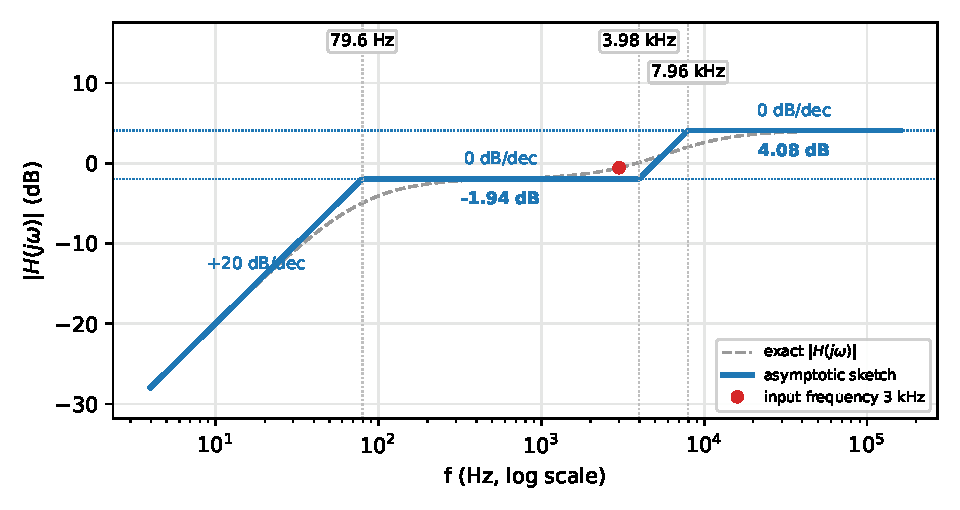
\includegraphics[width=0.78\linewidth,height=6.5cm,keepaspectratio]{p18_bode}\end{center}

{\small Blue: the straight-line sketch you are expected to draw. Dashed grey: the exact curve (about 3\,dB below the corner of an isolated pole). Red dot: the input frequency of Step 7.}
\solstep{7}{Steady-state output}The input is $V_i(t) = 0.1\sin\left(2\pi\cdot 3000\,t+\frac{\pi}{6}\right)$, so $\omega_{in} = 2\pi\cdot 3000 = 18800$\,rad/s. Put $s=j\omega_{in}$ in each factor (tool T5): magnitudes multiply, angles add.
{\small Rules: $\left|\frac{s}{s+p}\right| = \frac{\omega}{\sqrt{\omega^2+p^2}}$, $\angle = \frac{\pi}{2}-\tan^{-1}\frac{\omega}{p}$;\quad $\left|\frac{1}{1+s/p}\right| = \frac{1}{\sqrt{1+(\omega/p)^2}}$, $\angle = -\tan^{-1}\frac{\omega}{p}$;\quad $\left|1+\frac{s}{z}\right| = \sqrt{1+(\omega/z)^2}$, $\angle = \tan^{-1}\frac{\omega}{z}$;\quad a negative $K$ adds $-\pi$.}
\begin{center}\renewcommand{\arraystretch}{1.35}
\begin{tabular}{ccc}
\toprule
factor & magnitude & angle (rad) \\
\midrule
$-0.8$ & $0.8$ & $-3.14$ \\
$\rule[-1.1em]{0pt}{2.8em}\dfrac{s}{s+2\pi\cdot 79.6}$ & $0.9996$ & $0.0265$ \\
$\rule[-1.1em]{0pt}{2.8em}\left(1+\dfrac{s}{2\pi\cdot 3.98\mathrm{k}}\right)$ & $1.252$ & $0.646$ \\
$\rule[-1.7em]{0pt}{4em}\dfrac{1}{1+\dfrac{s}{2\pi\cdot 7.96\mathrm{k}}}$ & $0.9357$ & $-0.361$ \\
\textbf{total} & $\mathbf{0.9372}$ (product) & $\mathbf{-2.83}$ (sum) \\
\bottomrule
\end{tabular}\end{center}

\begin{align*}
|H(j\omega_{in})| &= 0.937, \qquad \angle H(j\omega_{in}) = -2.83\ \mathrm{rad} \\
v_{o,ac}(t) &= 0.937\times 0.1\,\sin\left(2\pi\cdot 3000\,t - 2.31\right) = 0.0937\,\sin\left(2\pi\cdot 3000\,t - 2.31\right)
\end{align*}

(phase: $\theta + \angle H = \frac{\pi}{6} + (-2.83) = -2.31$\,rad.)
\[
\boxed{V_o(t) = 0.0937\,\sin\left(2\pi\cdot 3000\,t - 2.31\right)\ \mathrm{V}}
\]

\begin{ansbox}
$H(s) = -0.8\,\dfrac{s}{s+2\pi\cdot 79.6}\,\left(1+\dfrac{s}{2\pi\cdot 3.98\mathrm{k}}\right)\,\dfrac{1}{1+\dfrac{s}{2\pi\cdot 7.96\mathrm{k}}}$\quad (corners: 79.6 Hz, 3.98 kHz, 7.96 kHz)\\[4pt]
$V_o(t) = 0.0937\,\sin\left(2\pi\cdot 3000\,t - 2.31\right)\ \mathrm{V}$
\end{ansbox}

\end{document}
